\documentclass[10pt]{beamer}

\usepackage[T1]{fontenc}
\usepackage{FiraSans} 


%
% Choose how your presentation looks.
%
% For more themes, color themes and font themes, see:
% http://deic.uab.es/~iblanes/beamer_gallery/index_by_theme.html
%
\mode<presentation>
{
  \usetheme[progressbar=foot,numbering=fraction,background=light]{metropolis}      % or try Darmstadt, Madrid, Warsaw, ...
  \usecolortheme{default} % or try albatross, beaver, crane, ...
  \usefonttheme{default}  % or try serif, structurebold, ...
  \setbeamertemplate{navigation symbols}{}
  \setbeamertemplate{caption}[numbered]
  %\setbeamertemplate{frame footer}{My custom footer}
} 

\usepackage[ngerman,english]{babel}
\usepackage{csquotes}
\usepackage[utf8x]{inputenc}


%--------------------------Editor mode.

\usepackage
[citestyle=authoryear,
%style=historian, 		%Loads the Historian files
sorting=nty,	  		%Sorts bibliography by year, name, title
autocite=footnote, 		%Autocite command generates footnotes
autolang=hyphen, 			%Allows hyphenation rules for foreign languages to apply to individual entries.						%(The other language rules should all be American)
mincrossrefs=1, 		%Includes all x-ref’ed entries in the bibliography
%usetranslator=true, 	%Translator’s name may be substituted for						%author or editor, if the latter are blank
%printseries, 			%Options provided by Historian, see below
backend=biber]
{biblatex}

\DeclareFieldFormat{postnote}{#1}
\DeclareFieldFormat{multipostnote}{#1}
\DeclareAutoCiteCommand{footnote}[f]{\footcite}{\footcites}

\bibliography{literature}
%----------------------------------------

%--------------------------Editor mode.


%\usepackage[default]{raleway}
\usepackage{fontawesome}


\usepackage{hyperref}
%\usepackage{enumitem} % produces fatal error with this template
%\setlist[itemize]{leftmargin=*} % belongs to enumitem

\usepackage{xcolor}
\definecolor{customcolor}{HTML}{616AC5}
\definecolor{alert}{HTML}{CD5C5C}
\definecolor{w3schools}{HTML}{4CAF50}
\definecolor{subbox}{gray}{0.60}
\definecolor{codecolor}{HTML}{FFC300}



 
%Information to be included in the title page:
\title[Digital Edition] %optional
{\vspace{0.5cm} Digital Editing \& XML/TEI }
\subtitle{for premodern books}
%\subtitle{Digital Editions with XPath \& XSLT for the Web \& in \LaTeX{}}
%\institute{\raggedleft
\includegraphics[height=1cm]{img/ninja-2000.png}\hspace{0.5cm}
\includegraphics[height=1cm]{img/harvard-logo.png} }
\author[SL]{\raggedleft Sarah Lang}
\date[2022] % (optional)
{\raggedleft 2022}

\logo{%\includegraphics[height=1cm]{unipassau.png}
%\includegraphics[height=1cm]{univie-logo.png}
%
\includegraphics[height=2cm]{zim.png}
}



\newcommand{\punkti}{~\lbrack\dots\rbrack~}

\renewenvironment{quote}
               {\list{\faQuoteLeft\phantom{ }}{\rightmargin\leftmargin}%
                \item\relax\footnotesize\ignorespaces}
               {\unskip\unskip\phantom{xx}\faQuoteRight\endlist}

\newcommand{\bgupper}[3]{\colorbox{#1}{\color{#2}\huge\bfseries\MakeUppercase{#3}}}
\newcommand{\bg}[3]{\colorbox{#1}{\bfseries\color{#2}#3}}

\newcommand{\mycommand}[2]{{\ttfamily\detokenize{#1}}~\dotfill{}~{\footnotesize #2}\\}

\newcommand{\sep}{{\scriptsize~\faCircle{ }~}}

\newcommand{\red}[1]{\bg{alert}{white}{#1}\\}
\newcommand{\green}[1]{\bg{w3schools}{white}{#1}\\}




%----------------------------------------------------------------------------------------------------------------


\usepackage{xcolor}
\definecolor{customcolor}{HTML}{616AC5}
\definecolor{alert}{HTML}{CD5C5C}
\definecolor{w3schools}{HTML}{4CAF50}
\definecolor{subbox}{gray}{0.60}
\definecolor{codecolor}{HTML}{FFC300}


%--------------------------------------------------------------------------------
\usepackage{tcolorbox}

\tcbuselibrary{most,listingsutf8,minted}

\tcbset{tcbox width=auto,left=1mm,top=1mm,bottom=1mm,
right=1mm,boxsep=1mm,middle=1pt}

\newenvironment{mycolorbox}[2]{%
\begin{tcolorbox}[grow to left by=-1em,grow to right by=-1em,capture=minipage,fonttitle=\large\bfseries, enhanced jigsaw,boxsep=1mm,colback=#1!30!white,on line,tcbox width=auto, toptitle=0mm,colframe=#1,opacityback=0.7,nobeforeafter,title=#2]\scriptsize%
}{\end{tcolorbox}\\[0.2em]}

\newenvironment{subbox}[2]{%
\begin{tcolorbox}[capture=minipage,fonttitle=\normalsize\bfseries, enhanced jigsaw,boxsep=1mm,colback=#1!30!white,on line,tcbox width=auto,left=0.3em,top=1mm, toptitle=0mm,colframe=#1,opacityback=0.7,nobeforeafter,title=#2]\scriptsize %
}{\normalsize\end{tcolorbox}\vspace{0.1em}}

\newenvironment{multibox}[1]{%
\begin{tcbraster}[raster columns=#1,raster equal height,nobeforeafter,raster column skip=1em,raster left skip=1em,raster right skip=1em]}{\end{tcbraster}}


\newenvironment{mycodebox}[2]{%
\begin{tcolorbox}[grow to left by=-1em,grow to right by=-1em,capture=minipage,fonttitle=\large\bfseries, enhanced jigsaw,boxsep=1mm,colback=#1!30!white,on line,tcbox width=auto, toptitle=0mm,colframe=#1,opacityback=0.7,nobeforeafter,title=#2]%
}{\end{tcolorbox}\\[0.2em]}

\newtcolorbox{mybox}[2][]{colback=codecolor!10!white,coltitle=red!70!black,
title={#2},fonttitle=\bfseries,#1}


%-------------------------------

\newtcblisting{mypy}[1]{colback=codecolor!5,colframe=codecolor!80!black,listing only, 
minted options={numbers=left, style=tcblatex,fontsize=\scriptsize,breaklines,autogobble,linenos,numbersep=3mm},
left=5mm,enhanced,
title=#1, fonttitle=\bfseries,
listing engine=minted,minted language=python}

\newtcblisting{myxml}[1]{colback=codecolor!5,colframe=codecolor!80!black,listing only, 
minted options={numbers=left, style=tcblatex,fontsize=\tiny,breaklines,autogobble,linenos,numbersep=3mm},
left=5mm,enhanced,
title=#1, fonttitle=\bfseries,
listing engine=minted,minted language=xml}

\newtcblisting{mybiggerxml}[1]{colback=codecolor!5,colframe=codecolor!80!black,listing only, 
minted options={numbers=left, style=tcblatex,fontsize=\footnotesize,breaklines,autogobble,linenos,numbersep=3mm},
left=5mm,enhanced,
title=#1, fonttitle=\bfseries,
listing engine=minted,minted language=xml}

\newtcblisting{myhtml}[1]{colback=codecolor!5,colframe=codecolor!80!black,listing only, 
minted options={numbers=left, style=tcblatex,fontsize=\tiny,breaklines,autogobble,linenos,numbersep=3mm},
left=5mm,enhanced,
title=#1, fonttitle=\bfseries,
listing engine=minted,minted language=html}

\newtcblisting{mycss}[1]{colback=codecolor!5,colframe=codecolor!80!black,listing only, 
minted options={numbers=left, style=tcblatex,fontsize=\tiny,breaklines,autogobble,linenos,numbersep=3mm},
left=5mm,enhanced,
title=#1, fonttitle=\bfseries,
listing engine=minted,minted language=css}


\newtcblisting{myjs}[1]{colback=codecolor!5,colframe=codecolor!80!black,listing only, 
minted options={numbers=left, style=tcblatex,fontsize=\tiny,breaklines,autogobble,linenos,numbersep=3mm},
left=5mm,enhanced,
title=#1, fonttitle=\bfseries,
listing engine=minted,minted language=js}



%------------------------------------------------------



\definecolor{bgcolour}{rgb}{0.95,0.95,0.95}
\newminted{sql}{fontsize=\footnotesize, 
                   linenos,
                   %fontfamily=fi4, 
                   numbersep=6pt,
                   autogobble,
                   %frame=lines,
                   bgcolor=black!8,
                   framesep=3mm} 

%\usemintedstyle[shell-session]{vim} %  vim monokai fruity native
% color=black!80
\newminted{shell-session}{fontsize=\scriptsize,numbersep=6pt,bgcolor=black!70,autogobble,framesep=3mm%  %frame=lines, %fontfamily=fi4, 
                   }                    
                   
\newminted{sparql}{fontsize=\scriptsize, 
                   %linenos,
                   %fontfamily=fi4, 
                   numbersep=6pt,
                   autogobble,
                   %frame=lines,
                   bgcolor=black!8,
                   framesep=3mm} 
                   
\newminted{turtle}{fontsize=\scriptsize, 
                   %linenos,
                   %fontfamily=fi4, 
                   numbersep=6pt,
                   autogobble,
                   %frame=lines,
                   bgcolor=black!8,
                   framesep=3mm} 
                   
\newminted{js}{fontsize=\scriptsize, 
                   linenos,
                   %fontfamily=fi4, 
                   numbersep=6pt,
                   autogobble,
                   %frame=lines,
                   bgcolor=black!8,
                   framesep=3mm}                    

\newminted{xml}{fontsize=\scriptsize, 
                   %linenos,
                   %fontfamily=fi4, 
                   numbersep=6pt,
                   autogobble,
                   %frame=lines,
                   bgcolor=black!8,
                   framesep=3mm} 
                   
\newminted{tex}{fontsize=\scriptsize, 
                   %linenos,
                   %fontfamily=fi4, 
                   numbersep=6pt,
                   autogobble,
                   %frame=lines,
                   bgcolor=black!8,
                   framesep=3mm} 
                   
\newminted{postscript}{fontsize=\scriptsize, 
                   %linenos,
                   %fontfamily=fi4, 
                   numbersep=6pt,
                   autogobble,
                   %frame=lines,
                   bgcolor=black!8,
                   framesep=3mm} 
                   
\newminted{html}{fontsize=\scriptsize, 
                   %linenos,
                   %fontfamily=fi4, 
                   numbersep=6pt,
                   autogobble,
                   %frame=lines,
                   bgcolor=black!8,
                   framesep=3mm} 
                   
\newminted{css}{fontsize=\scriptsize, 
                   %linenos,
                   %fontfamily=fi4, 
                   numbersep=6pt,
                   autogobble,
                   %frame=lines,
                   bgcolor=black!8,
                   framesep=3mm} 
                   

%-------------------------------  
% https://tex.stackexchange.com/questions/377777/why-do-my-beamer-blocks-without-title-still-have-a-background
\usepackage{xstring}                
\setbeamertemplate{block begin}
{
  \par\vskip\medskipamount%
  \IfStrEq{\insertblocktitle}{}{}{
      \begin{beamercolorbox}[colsep*=.75ex]{block title}
        \usebeamerfont*{block title}\insertblocktitle%
      \end{beamercolorbox}%
  }
  {\parskip0pt\par}%
  \ifbeamercolorempty[bg]{block title}
  {}
  {\ifbeamercolorempty[bg]{block body}{}{\nointerlineskip\vskip-0.5pt}}%
  \usebeamerfont{block body}%
  \begin{beamercolorbox}[colsep*=.75ex,vmode]{block body}%
    \ifbeamercolorempty[bg]{block body}{\vskip-.25ex}{\vskip-.75ex}\vbox{}%
}
%-------------------------------  


\usepackage{multicol}
\usepackage{hyperref}
\usepackage[normalem]{ulem} % for strikethrough


\begin{document}
%------------------------------------------------------------------------------
% FRONT
%------------------------------------------------------------------------------
{
\usebackgroundtemplate{
\includegraphics[width=\paperwidth]{img/kfu-zim-slides.png}}
\frame{\titlepage}
}
%\frame{\titlepage}
\setcounter{tocdepth}{1}
%------------------------------------------------------------------------------
\begin{frame}{Overview}%\scriptsize
  \setbeamertemplate{section in toc}[sections numbered]
  \begin{small}
  \begin{multicols}{2}\tableofcontents\end{multicols}
  % on toc formatting:
  % https://tex.stackexchange.com/questions/26929/two-column-beamer-toc-with-control-over-the-breaking-point
  \end{small}
\end{frame}
%------------------------------------------------------------------------------

\metroset{block=fill}
%

\section{Syllabus}
%------------------------------------------------------------------------------
\begin{frame}{Content}
\begin{block}{Theoretical and practical introduction to digital scholarly editing:}

\begin{enumerate}\small
    \item what is a digital scholarly edition?
    \item who do I encode an edition in XML/TEI?
    \item what paradigms exist in digital scholarly editing?
\end{enumerate}
\end{block}

\footnotesize
Preparing historical documents for research is a core task in many humanities disciplines. The result of this work, the `scholarly edition', has seen fundamental changes due the use of digital technologies: Not only did a new, digital publishing medium take the place of paper, but new forms of analysis, semantization, research and the production of multiple representation formats based on one edition (text) source have been developed (\emph{single source principle}). 
The course serves as an introduction into the scholarly debate on the issue. It covers both theoretical foundations as well as working on practical examples coming from the participants' scholarly domain of origin. Furthermore, it introduces fundamental technologies like XML/TEI or transcription using Transkribus.

\begin{block}{Main learning goal}
Participants are able to recognize basic approaches and issues in the context of digital edition and to apply them to their own scientific domain in practical work.
\end{block}

\end{frame}
 
\section{Preliminaries}
%------------------------------------------------------------------------------
\begin{frame}{How to get a positive grade on this class}
\subsection{Grading}

  \begin{columns}[T,onlytextwidth]
    \column{0.48\textwidth}
      \begin{exampleblock}{Final Submission (60\%)}
\begin{itemize}\footnotesize
\item \textbf{Infomod:} Text, ER model, SQL database
\item \textbf{DigEd:} Small digital edition or review of an existing edition.
\item You can start in the last month of the semester and ask questions.
\item You can collaborate but no plagiarism (Uni Graz zero tolerance policy).
\end{itemize}
\end{exampleblock}

\begin{exampleblock}{Homework assignments (40\%)}\footnotesize
Communicated and to be completed within the week
\end{exampleblock}

    \column{0.48\textwidth}
      \begin{alertblock}{Other aspects}
\begin{enumerate}\scriptsize
    \item attendance in class (you can miss max. 3, to be communicated beforehand).
    \item Positive grade: at least 50\%  on all partial submissions.
    \item ``LVen mit immanentem Prüfungscharakter'' $\to$ once you accept the first task you get a grade (i.e. first homework this week)
    \item If you get a negative grade, the whole class needs to be retaken.
\end{enumerate}

\begin{quote}\scriptsize
    Nichterbringung weiterer Teilleistungen ohne wichtigen Grund ist Prüfungsabbruch (Negativbeurteilung). Abmeldung nach bereits übernommener Teilleistung führt zu negativer Beurteilung.
\end{quote}
\end{alertblock}

\end{columns}

\small 
see also: slides on grading \& further info materials on the final submission
    
\end{frame}


%------------------------------------------------------------------------------
\begin{frame}{Deadlines}

\begin{alertblock}{Hard deadlines}\small
\textbf{All deadlines are hard deadlines.}  You can get extensions for good reasons. 
\begin{itemize}
\item Good reasons for example: care responsibility, being ill, etc.
\item i.e. understandable reasons which are communicated asap
\end{itemize}

\end{alertblock}

\begin{alertblock}{If you miss a deadline\dots}
\begin{itemize}\small
\item If you didn’t communicate: negative grade.
\item Otherwise up for discussion according to the circumstances.
\end{itemize}
\end{alertblock}

\end{frame}
%------------------------------------------------------------------------------
\begin{frame}{Learning Goals}
\subsection{Learning Goals}
\begin{enumerate}
    \item Participants are able to recognize basic approaches and issues in the context of digital edition and to apply them to their own scientific domain in practical work.
    \begin{itemize}
        \item knowledge of theoretical basics
        \item being able to judge the quality of a digital scholarly edition
        \item being able to encode a DSE in XML/TEI
    \end{itemize}
    \item XML/TEI for digital scholarly editions
    \item some special cases such as encoding critical apparatus or zones
\end{enumerate}

\metroset{block=fill}
\begin{alertblock}{Final project}
\footnotesize
Small digital edition or review of an existing edition following the reviewing guidelines by the journal RIDE. To be submitted February 15th.

\end{alertblock}
\end{frame}


%------------------------------------------------------------------------------
\begin{frame}{Working with computers as a humanities person}

\begin{itemize}
    \item \href{https://static.uni-graz.at/fileadmin/gewi-zentren/Informationsmodellierung/PDF/U__bungsblatt-0.pdf}{Übungsblatt 0} is a prerequisite
    \item don't panic
\end{itemize}
    
\end{frame}

%------------------------------------------------------------------------------
\begin{frame}[standout]
    \alert{Present yourselves! } \\
    \normalsize
    Name, pronouns, domain of origin, interests, etc. \\
    Previous knowledge in Digital Humanities, scholarly editing, XML/TEI?
\end{frame}


%------------------------------------------------------------------------------
%\begin{frame}[standout]    Resources\end{frame}
\subsection{Resources}
%------------------------------------------------------------------------------
\begin{frame}[allowframebreaks]{References}
\begin{enumerate}\footnotesize
    \item Patrick \textbf{Sahle:} \emph{Digitale Editionsformen. Zum Umgang mit der Überlieferung unter den Bedingungen des Medienwandels, Schriften des Instituts für Dokumentologie und Editorik} (Norderstedt, 2013)
    \item Patrick \textbf{Sahle:} \emph{Digitale Editionstechniken}, in: Martin Gasteiner und Peter Haber (Hrsg.), \emph{Digitale Arbeitstechniken für die Geistes- und Kulturwissenschaften.} Wien: UTB, 2009.
    \item Patrick \textbf{Sahle:} \emph{Zwischen Mediengebundenheit und Transmedialisierung. Anmerkungen zum Verhältnis von Edition und Medien.} In: \emph{editio} 24 (2010), 23--36. DOI 10.1515/edit.2010.004
    \item Elena \textbf{Pierazzo:} \emph{What Future for Digital Scholarly Editions? From Haute Couture to Prêt-à-Porter}, \emph{International Journal of Digital Humanities} 1.2 (2019), 209--220. \protect\url{https://doi.org/10.1007/s42803-019-00019-3}
    \item Elena \textbf{Pierazzo:} \emph{Digital Scholarly Editing}, Farnham u.a. 2015.
    \item Matthew James \textbf{Driscoll} \& Elena \textbf{Pierazzo (eds.):} \emph{Digital Scholarly Editing. Theory, Practice and Future Perspectives} (Open Book Publishers, 2016). \protect\url{https://doi.org/10.11647/OBP.0095}
    \item Marilyn \textbf{Deegan} \& Kathryn \textbf{Sutherland (eds.):} Text Editing, print and the Digital World, Aldershof/UK 2009 (Digital Research in Arts and Humanities).
    \item Special Issue `Digital Scholarly Edition' of the \emph{International Journal of Digital Humanities} 1, Nr. 2 (2019); \href{https://link.springer.com/journal/42803/topicalCollection/AC_00bb5c504ba4a0bbaa9dc32f1881a986}{<Link>}.
    \item Mats \textbf{Dahlström:} How Reproductive is a Scholarly Edition? In: \emph{Literary and Linguistic Computing} 19/1 (2004), S. 17-33. 
    \item Mats \textbf{Dahlström:} ``Critical editing and critical digitization''. In: E. Thoutenhoofd, A. van der Weel \& W. Th. van Peursen (eds.), \emph{Text comparison and digital creativity: the production of presence and meaning in digital text scholarship.} Amsterdam: Brill, 2010, 79--97.
    \item Peter \textbf{Robinson:} ``Towards a Theory of Digital Editions'', in: \emph{Variants} 10 (2013).
    \item Susan \textbf{Schreibman:} \emph{Digital Scholarly Editing}, in: \emph{Literary Studies in the Digital Age: An evolving anthology}, Kenneth M. Price \& Ray Siemens (eds.), 2014.  \protect\url{http://dlsanthology.commons.mla.org/digital-scholarly-editing/}
    \item M. N. \textbf{Smith:} Electronic scholarly editing, in: A Companion to Digital Humanities, Susan Schreibman, Raymond George Siemans \& John Unsworth eds., Malden 2004, 306--322.
    \item More references: \protect\url{http://www.hgw-online.net/GHWBibliographie/systematik/Editionstechnik}
\end{enumerate}

\end{frame}

%------------------------------------------------------------------------------
\begin{frame}{Ressources}

\begin{enumerate}
    \item \textbf{OxygenXML:}
    \begin{itemize}
        \item \href{https://www.oxygenxml.com/}{oXygen XML editor}
        \item \href{https://www.oxygenxml.com/xml_editor/download_oxygenxml_editor.html}{Download oXygen XML}
        \item to use this, you will need a license key $\to$ Moodle
    \end{itemize}
    \item \textbf{XML/TEI}
    \begin{itemize}
        \item \href{https://tei-c.org/}{Text Encoding Initiative (TEI)}
        \item \href{https://de.wikipedia.org/wiki/Text_Encoding_Initiative}{TEI Wikipedia}
        \item German intro video using OxygenXML: \href{https://www.youtube.com/watch?v=fnVV9N4kkQ8}{TEI-Annotation in Oxygen XML: Von den Basics zur Automatisierung mit regulären Ausdrücken} $\to$ switch on auto-generated subtitles
        \item Blog post \href{https://latex-ninja.com/2022/02/02/a-shamelessly-short-intro-to-xml-for-dh-beginners-includes-tei/}{\emph{A shamelessly short intro to XML for DH beginners (includes TEI)}, \LaTeX{}-Ninja Blog} (02.02.2022).
        \item \href{https://www.w3schools.com/xml/}{W3Schools step-by-step XML tutorial}
    \end{itemize}
    \item \textbf{Critical Apparatus Toolbox:}
    \begin{itemize}
        \item \href{https://web.archive.org/web/20191211173459/http://teicat.huma-num.fr/}{Marjorie Burghart’s TEI Critical Apparatus Toolbox}
        \item \href{https://doi.org/10.4000/jtei.1520}{Marjorie Burghart, \emph{The TEI Critical Apparatus Toolbox: Empowering Textual Scholars through Display, Control, and Comparison Features}, in \emph{jTEI} 10: \protect{https://doi.org/10.4000/jtei.1520}}
    \end{itemize}
    
\end{enumerate}

\end{frame}

%------------------------------------------------------------------------------
\begin{frame}{First homework assignment}

\begin{itemize}
    \item Please read: \\ 
    Patrick \textbf{Sahle:} ``What is a scholarly digital edition (SDE)?'' In: \emph{Digital Scholarly Editing. Theory, Practice and Future Perspectives.} Ed. by Matthew Driscoll and Elena Pierazzo. Cambridge: Open Book Publishers, 2016, 19--39.  \protect\url{https://books.openedition.org/obp/3397?lang=en}
    \item Write a short reflection on the text in which you try to explain the difference between a digital and a non-digital edition.
    \item Make sure to keep your musings to maximum 1-2 pages of text! 
    \item The deadline is this Saturday night! (23:59)
    \item Careful -- by submitting this homework, you take on the first assignment and therefore, will receive a grade on this class even if you drop out!
\end{itemize}
    
\end{frame}



%------------------------------------------------------------------------------
% MAIN
%------------------------------------------------------------------------------

%-----------------------------------------------------
\section{The TEI \& Digital Editing Session}

\begin{frame}{Goals}
\subsection{Goals}
\begin{enumerate}
    \item understand basic modelling theory for digitization 
    \item understand the differences between a digital scholarly edition \& other digital resources (such as archives or library catalog data)
    \item understand the role of XML/TEI in Digital Editing
    \item be able to use the Text Encoding Initiative standard to encode descriptions of pre-modern books
\end{enumerate}

\metroset{block=fill}
    \begin{block}{Goals for the next session}
    \begin{enumerate}
        \item understanding modelling theory relevant for digitization
        \item understanding the terms `digital edition', `digital archive' versus library catalogs
        \item[\textcolor{alert}{\faClose}] \texttt{<msDesc>} $\to$ next session
        \item[\textcolor{alert}{\faClose}] transcriptions in TEI \& Transkribus $\to$ later session
    \end{enumerate}
    \end{block}
\end{frame}


%-----------------------------------------------------






\section{Data modelling}


%------------------------------------------------------------------------------
\begin{frame}[allowframebreaks]{3 proporties of a model following Stachowiak}

\metroset{block=fill}
\begin{alertblock}{1)~ Mapping }
\begin{quote} \scriptsize
    „Modelle sind stets Modelle von etwas, nämlich Abbildungen, Repräsentationen natürlicher oder künstlicher Originale, die selbst wieder Modelle sein können.“ 
    %„Originale und Modelle werden hier ausschließlich als Attributklassen gedeutet, die oft die spezielle Gestalt attributiver Systeme erlangen.“ % 131
    „Der Abbildungsbegriff fällt mit dem Begriff der Zuordnung von Modell-Attributen zu Original-Attributen zusammen.“ \parencite[131--132]{stachowiak} % 132
    
    \alert{Models are always models of something, i.e. mappings from, representations of natural or artificial originals, that can be models themselves.}
\end{quote}
\end{alertblock}
\begin{alertblock}{2)~ Reduction}
\begin{quote} \scriptsize
    „Modelle erfassen im allgemeinen nicht alle Attribute des durch sie repräsentierten Originals, sondern nur solche, die den jeweiligen Modellerschaffern und/oder Modelbenutzern relevant scheinen.“ \parencite[132]{stachowiak}
    
    \alert{Models in general capture not all attributes of the original represented by them, but rather only those seeming relevant to their model creators and/ or model users.}
\end{quote}
\end{alertblock}
\framebreak 

\begin{alertblock}{3)~ Pragmatism}
\begin{quote} \scriptsize
    „Eine pragmatisch vollständige Bestimmung des Modellbegriffs hat nicht nur die Frage zu berücksichtigen, \emph{wovon} etwas Modell ist \lbrack{}Abbildungsmerkmal\rbrack{}, sondern auch, \emph{für wen, wann} und \emph{wozu} bezüglich seiner je spezifischen Funktionen es Modell ist.“ \parencite[132]{stachowiak} % 132
    
    \alert{ Models are not uniquely assigned to their originals per se. They fulfill their replacement function \\
    a) for particular – cognitive and/ or acting, model using subjects, \\
    b) within particular time intervals and \\
    c) restricted to particular mental or actual operations.}
\end{quote}
\end{alertblock}

\end{frame}

%------------------------------------------------------------------------------
\begin{frame}{Stachowiak's \emph{General Model Theory}}

\begin{block}{Stachowiak's notion of a model}
\begin{quote}
    Alle Erkenntnis ist Erkenntnis in Modellen oder durch Modelle und jede menschliche Weltbegegnung überhaupt bedarf des Mediums Modell.
\end{quote}
\alert{$\to$ All knowledge-making is knowledge-making in or through models and all human perception of the world needs models as a medium. }
\end{block}

\begin{block}{Data modelling}\small
Model = snippet of the real world but it only covers the attributes I chose to be relevant for the task at hand. 
Thus, the model and the aspect of the real world it models (its subject) diverge. 
\end{block}

\begin{block}{Digital, standardized \& formal models}\small 
Standardized models allow us to exchange and analyse data, search/query data. 
 $\to$ only \emph{formal models} can be processed digitally, i.e. every digital model is a formal model.
\end{block}

\alert{$\to$ Models are simplified representations of parts of the real world.}

\end{frame}

%------------------------------------------------------------------------------
\begin{frame}{Why should we care about modelling theory?}
    \begin{itemize}
        \item Modelling is a pivotal task in the Digital Humanities.
        \item When we create digital representations of material objects, those are models. 
        \item Models are by definition subjective, abstracted and not universal. 
        \item Their quality has to be judged in relation to their purpose (Stachowiak's 3rd criterion): $\to$
    \end{itemize}
\end{frame}


%------------------------------------------------------------------------------
    \begin{frame}{Different motivations for digital projects}
    \begin{block}{research-driven:}\small
        individualized for answering a research question, work-intensive \& relatively expensive.
    \end{block}

    \begin{block}{curation-driven}\small
        mass-digitization, cookie cutter approach which covers the most important elements for most use cases but can easily miss features relevant to subject-matter experts.
            \begin{itemize}\footnotesize
                \item despite the objects being digitized, users might have to go back to the material objects to fill in the blanks
                \item but objects become more discoverable \& (hopefully) somewhat comparable to larger corpora of similar objects
                \item superficial digitization can lead to the creation of misleading datasets, e.g. errors or bad tagging $\to$ \alert{reparative librarianship} is needed
                \item potential application for machine learning approaches
            \end{itemize}
    \end{block}

\end{frame}


%------------------------------------------------------------------------------
\begin{frame}{What are data?}
\metroset{block=fill}
\begin{block}{Definitions of `data'}
Plural of Latin \emph{datum} ('given'). 
\end{block}

\begin{itemize}\footnotesize 
    \item data aren't exactly a given but rather constructed or created.
    \item There has been a discussion in the DH whether we should call them \emph{capta}~\parencite{Drucker2011dataCapta}
    \item Most data (so-called `givens') are constructed by phenomenotechnical devices~\parencite{bachelard1968}, i.e. pereiving devices which translate the (often quite abtract) things they see into data.
    \item data has to be interpreted.
    \item Stachowiak's pragmatism criterion means we selectively capture data most important to us, not all possible aspects (!).
\end{itemize}

Data resulting from cataloging \& digitization contains interpretations \& is thus, 
\emph{per definitionem} always subjective \& incomplete (!).

\alert{data $\neq$ original!}

\end{frame}



% Teaser: Why are we here? General terms: digital edition and archive
%-----------------------------------------------------
\section{Digital Scholarly Editing}

\subsection{Theory \parencite{sahleDigitalEdition2016}}
%-----------------------------------------------------
\begin{frame}[allowframebreaks]{What is a Digital Scholarly Edition?}
\metroset{block=fill}\small
Digital editions (as per \cite{sahleDigitalEdition2016}):
        \begin{itemize}
            \item discipline-independent \& not exclusive to text
            \item overcome the limitations of print (financial, inter-/ multimediality, etc.)
            \item follow a digital paradigm like printed editions follow the print paradigm (``shaped by the technical limitations and cultural practices'')
            \item ``A digitised edition is not a digital edition.'' $\to$ it's not about the storage medium (just being on the internet doesn't make it a digital edition!)
            \item ``A digital edition cannot be given in print without significant loss of content and functionality.''
            \begin{itemize}\footnotesize
                \item different views, interactivity, searchability
                \item facsimiles alongside diplomatic transcription and reading versions
                \item all generated from the same source data: \textbf{single source principle} $\to$ How? Data transformation!
                \item $\neq$ Digital Archive,  text corpus or facsimile $\to$ has critical engagement 
            \end{itemize}
        \end{itemize}

\framebreak

We need to start at the beginning: 

\begin{block}{What is a scholarly edition?}
\begin{itemize}
    \item originally stems from ecdotics (\emph{ecdotica, ecdotique, Editorik / Editionswissenschaft}) $\to$ tradition of Philology
    \item \textbf{goal = textual criticism}: reconstruct the original version of a text transmitted to us via textual witnesses (\emph{Lachmannian paradigm})
\end{itemize}
\end{block}

\begin{block}{\cite{sahleDigitalEdition2016}}
    \begin{quote}
        A scholarly edition is the critical representation of historic documents. % \parencite{sahleDigitalEdition2016}. 
        
        \emph{Edition ist die erschließende Wiedergabe historischer Dokumente.}
    \end{quote}
\end{block}

\framebreak 
    
Criteria from \cite{sahleDigitalEdition2016}:
    \begin{enumerate}\footnotesize
        \item \textbf{Representation:} recoding a document and its transformation (in the same or other media)
        \begin{itemize}\scriptsize
            \item Visually: image reproduction, facsimile
            \item Textually: transcription.
            \item varying degrees of closeness/abstraction with regard to the original document
        \end{itemize}
        \item representation $\neq$ presentation
        \item \textbf{Critical engagement} (based on scholarly agenda). ``Critical engagement without representation is not an edition–but an examination, a catalogue or a description.''
        \begin{itemize}\scriptsize
            \item textual criticism
            \item historic criticism
            \item bibliographic criticism
            \item material criticism
            \item visual criticism
            \item etc.
        \end{itemize}
        \item \textbf{Documents:} ``every non-abstract object that is the subject of an edition can be called a document.''
        \item \textbf{Historic:} editions ``explain what is not evident to the present-day reader. In short, they bridge a distance in time, a historical difference. Texts that are created today do not need to be critically edited. They can speak for themselves.''
    \end{enumerate}

\begin{block}{\cite{sahleDigitalEdition2016}}    
    \begin{quote}
        A representation without \lbrack{}critical\rbrack{} treatment or the addition of information is not an edition–but a facsimile, a reproduction or–nowadays–a digital archive or library. 
        
        \textbf{Critical representation} as a compound notion of editing aims at the reconstruction and reproduction of texts and as such addresses their material and visual dimension as well as their abstract and intentional dimension \parencite{sahleDigitalEdition2016}. 
    \end{quote}
\end{block}

\framebreak

Questions to ask if you want to know if it's a Digital Scholarly Edition:
\begin{enumerate}
    \item \textbf{Is there a full representation} of the subject in question?
    \item \textbf{Is it critical?} $\to$ processing rules stated and applied, scholarly knowledge included to make the document easier to understand, regarding material, document genesis/creation, context and reception?
    \item \textbf{Is the edition of academic quality?} $\to$ transparent and rigorous edition process, responsibilities stated, enables future research on a reliable basis.
    \item \textbf{Does the edition follow a digital paradigm?} $\to$ makes use of the possibilities of the digital, not printable without major loss of content or functionality.
\end{enumerate}

\framebreak

\begin{alertblock}{Ideally, a DSE should also implement the FAIR criteria}
\begin{description}\footnotesize
    \item[Findable.] in library catalogs, discovery systems or repositories, with a persistent identifier
    \item[Accessible.] free for any user, no access restrictions? (from open access to usability, language selection, etc.) 
    \item[Interoperable.] data in standardized and widely used format (for example TEI or similar standards), allowing for reuse and data exchange outside of the project. 
    \item[Reusable.] data accessible (individual download, aggregate download, repository, API)? Licenses allowing reuse. Data creation, modelling and processing documented adequately so that others can make sense of it? 
\end{description}
\end{alertblock}

$\to$ \href{https://ride.i-d-e.de/}{RIDE (review journal for digital editions and resources)} \\
$\to$ \href{https://ride.i-d-e.de/reviewers/catalogue-criteria-for-reviewing-digital-editions-and-resources/}{RIDE Criteria for Reviewing Digital Editions and Resources}
\end{frame}

%-----------------------------------------------------

\begin{frame}{Further reading}
    \fullcite{sahleDigitalEdition2016}
    \bigskip 
    
  \begin{block}{Blogpost (short summary)}\footnotesize \href{https://latex-ninja.com/2022/10/30/what-you-really-need-to-know-about-digital-scholarly-editing/}{\emph{What you really need to know about Digital Scholarly Editing}, The \LaTeX{} Ninja Blog, 30.10.2022.} = \parencite{LaTeXNinjaDSE2022}
  \end{block}
    
\end{frame}
%-----------------------------------------------------

\section{Editorial Schools and Workflows}

\begin{frame}{What is a text?}
    Patrick Sahle's text wheel
    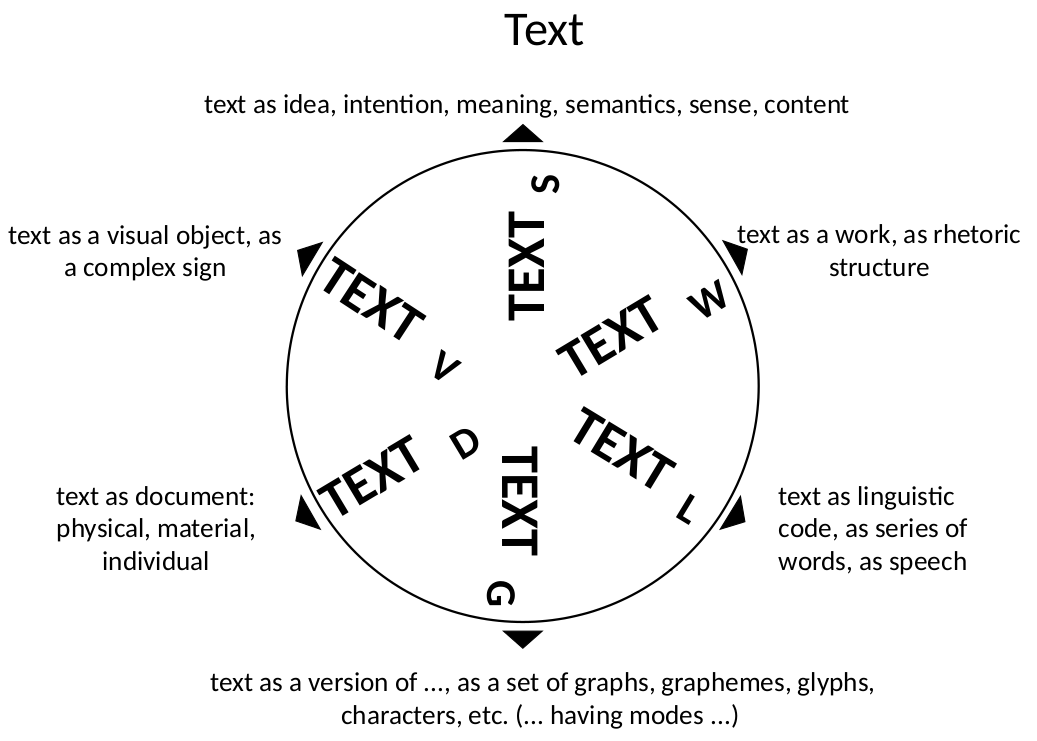
\includegraphics[width=0.95\textwidth]{img/sahle-text-wheel.png}
\end{frame}
%-----------------------------------------------------
\begin{frame}[allowframebreaks]{Edition workflows and schools}
\subsection{Steps involved in DSE}

{\scriptsize
The following slides are adapted from Georg Vogeler's slides on digital editing.
}
\metroset{block=fill}\footnotesize
\begin{columns}
\column{0.65\textwidth}
\begin{block}{Traditional Workflow of Philological Editing}
\begin{itemize}
    \item \textbf{Heuristics:} Find your textual witnesses
    \item \textbf{Transcription:} transfer the text into your prefered alphabet (from the original/from a photo)
    \item \textbf{Collation:} Compare the textual witnesses
    \item \textbf{Recensio:} Evaluate the variants and create a stemma (commenting)
    \item Write your introduction
    \item Typesetting
    \item Create an index (refering to pages)
    \item Print and distribution
\end{itemize}
\end{block}

\column{0.33\textwidth}
\begin{block}{In the digital realm:}
\begin{itemize}
    \item edition 
    \item beta version
    \item just TEI data publication
    \item hybrid (web and print) publication
    \item minimal edition (adaptation from \href{https://go-dh.github.io/mincomp/about}{minimal computing})
\end{itemize}
\end{block}

\alert{A digital edition is social, iterative, a process\dots }
\end{columns}

\framebreak


\begin{columns}
\column{0.48\textwidth}
\begin{block}{„Edition“}
\begin{itemize}
\item  a particular version of a book
\item  a particular version of a product
\item  all the copies of a book that are printed or published at one time
\end{itemize}
\end{block}

\begin{block}{„Historical-critical“ Edition}
\begin{itemize}
\item  Documentation of the history of the text
transmission in the “apparatus of variants”
\item  Critical evaluation of the textual transmission
\end{itemize}
\end{block}

\column{0.48\textwidth}
\begin{block}{Patrick Sahle's text wheel}
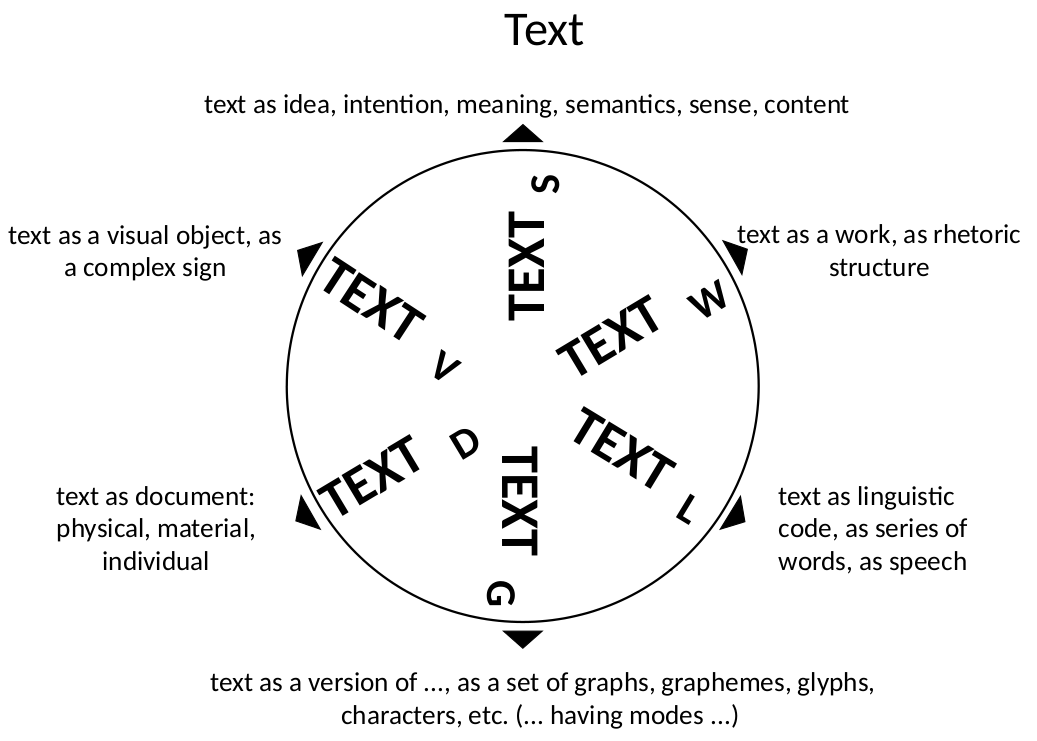
\includegraphics[width=\textwidth]{img/sahle-text-wheel.png}
\end{block}

\begin{block}{Karl Lachmann (1793--1851)}
\textbf{Editorial intervention:} Philological knowledge (linguistics, style) allows us to emend fragmentary textual transmission.
\end{block}
\end{columns}

\framebreak

\begin{block}{Editorial Schools}
\begin{multicols}{2}
\begin{itemize}
\item Lachmann (`Historisch-Kritische Ausgabe', stemmatology)
\item Reading text vs. critical edition = reader-oriented pragmatism / modernised edition / `reading text'
\item  Last authorized edition
\item  First edition / \emph{editio princeps}
\item Main manuscript (Bédier 1937, `Leithandschrift')
\item `diplomatic edition / transcription'
\item Typographic/photographic facsimile
\item `documentary editing' (Tanselle)
\item variorum edition
\item genetic edition / \emph{critique génétique} (Gabler)
\item Copy-Text-Theory (Greg 1950/3, Bowers 1976, 1978)
\item New Philology (Stackmann 1964, 1993, 1994, 1999; Ruh 1978, Cerquiglini 1989)
\end{itemize}
\end{multicols}
\end{block}

\end{frame}




%-----------------------------------------------------

\begin{frame}[standout]

  \alert{If you wanted to practice\dots}
  
  \normalsize
  \href{https://ride.i-d-e.de/reviewers/call-for-reviews/}{Write a RIDE review} on a digital edition \alert{\href{https://ride.i-d-e.de/reviewers/suggested-projects-for-review/}{(suggestions for review)}} according to their \alert{\href{https://ride.i-d-e.de/reviewers/submission-guidelines/}{review criteria}}!
  
  \footnotesize (If you actually plan on submitting, contact the editors first. 2000 words minimum, project from your field. Peer-review can spot things you're unsure about.)
\end{frame}

% Patrick Sahle (Göttingen). Digitales Archiv – Digitale Edition. Anmerkungen zur Begriffsklärung

\section{Digital Archives}
\begin{frame}{Digital long-term archiving}
\metroset{block=fill}\footnotesize
\begin{columns}
\column{0.68\textwidth}
\begin{itemize}
\item ensuring the authentic and sustainable availability of digital ressources on the level of the bitstream and on a semantic level
\item integral principle to every form of sustainable data storage
\item begins with the data production in a sustainable data format (and ideally, following a recognized data standard)
\item requires standardization of data formats and archiving workflows
\item serves both the dissemination as well as the preservation of digital content
\item not just about technical solutions but also institutional stability and policies
\end{itemize}
\column{0.28\textwidth}

\begin{block}{A digital archive}
\begin{itemize}
\item is more than a mere collection of scanned book pages or digitized images, etc.
\item if offers metadata, norm data and controlled vocabularies
\end{itemize}
\end{block}

\end{columns}
\end{frame}
%---------------------------------


\begin{frame}{Digital Archives}
\metroset{block=fill}\footnotesize
\begin{columns}
\column{0.55\textwidth}
\begin{block}{Digital Archive}
\begin{itemize}
\item organized collection of digital objects (text, images, audio, video and multimedia streams)
\item digital objects are described by standards both in terms of contents (e.g. TEI) and bibliographically (e.g. Dublin Core)
\item published sustainably using interfaces, services and APIs (e.g. OAI-PMH)
\item digital objects have unique, persistent and citable identifiers (e.g. DOI, URN, PURL, PID)
\item authenticity of objects is checked by means of digital signatures or checksums (`Is the number of bytes in the object still the same it used to be?')
\end{itemize}
\end{block}
\column{0.43\textwidth}
\begin{block}{Trustworthy Digital Archives}
as defined by the Research Libraries Group (RLG)
\begin{itemize}
\item secure organizational structure and legal status
\item financial sustainability
\item technological and procedural aptness
\item ensuring data and system security
\item documentation and transparency
\item conformity with the OAIS standard
\end{itemize}
\end{block}
\end{columns}
$\to$ retro-digitizing objects but also standards for new (born digital) resources.
\end{frame}

%---------------------------------

\begin{frame}{Digital Archives vs. Digital Editions~\parencite{sahleArchiv2007} }
\metroset{block=fill}
\footnotesize
\begin{columns}
\column{0.38\textwidth}

\begin{block}{Digital documents}\scriptsize
Material objects are the target of digitization but digitization doesn't reproduce them -- it represents them in a digital format.
A digital document is a view on the original material object.
\end{block}

\begin{block}{Archive}\scriptsize
Traditionally an archive is an ordered collection of documents with the goal of documenting them, preserving them in the long-term and making them accessible. 
$\to$ this function isn't only carried out by actual archives but also by  museums, libraries and other cultural heritage institutions. 
Traditional archive material doesn't need to be represented because its physical objects can be accessed directly. 
\end{block}

(we have already def'd editions)

\column{0.6\textwidth}
\scriptsize
Editions are often based in archival material. The edition isn't a storage device, it is a publication of a historical source and the editorial work done on it. 
While the edition contains lots of editorial work and enrichment, archival documents are usually original and largely unprocessed. A non-digital archive isn't a form of publication in and of itself -- a digital archive \emph{is} a form of publication, too, like a digital edition 
$\to$ blurs the lines a bit. 

We could say that \textbf{the difference lies in the depth of data enrichment and editorial work.} $\to$ once a presentation form is provided, data from a digital archive becomes a digital edition.
% erschließende Wiedergabe. 

% Dahlström, Mats: How Reproductive is a Scholarly Edition? In: Literary and Linguistic Computing 19/1 (2004), S. 17–33.

% Robinson, Peter: What is a Critical Digital Edition? In: Variants. Journal of the European Society for Textual Scholarship 1 (2002), S. 43–62.

\begin{block}{Digital Archive}\scriptsize
A main goal of a digital archive is to preserve and publish a specific choice of documents as a collection (ideally, representative and well-balanced). The digital objects aren't necessarily direct representations but may have undergone editorial intervention (e.g. normalized orthography). 
Its documents should be uniform in how they are encoded and processed.
In the case of the single source principle, the edition is generated dynamically (`on the fly') from the archived source data. (If any edition is provided).
\end{block}

\end{columns}

\end{frame}
%---------------------------------



\section{Library catalog data}
\begin{frame}{Theuerdank (Graz Sondersammlungen -- Rara 1 III 11723 )}
\footnotesize
    Pfintzing, Melchior, et al. Die geuerlicheiten und einsteils der geschichten des loblichen streytparen und hochberümten helds und Ritters herr Tewrdannckhs. 1517.

    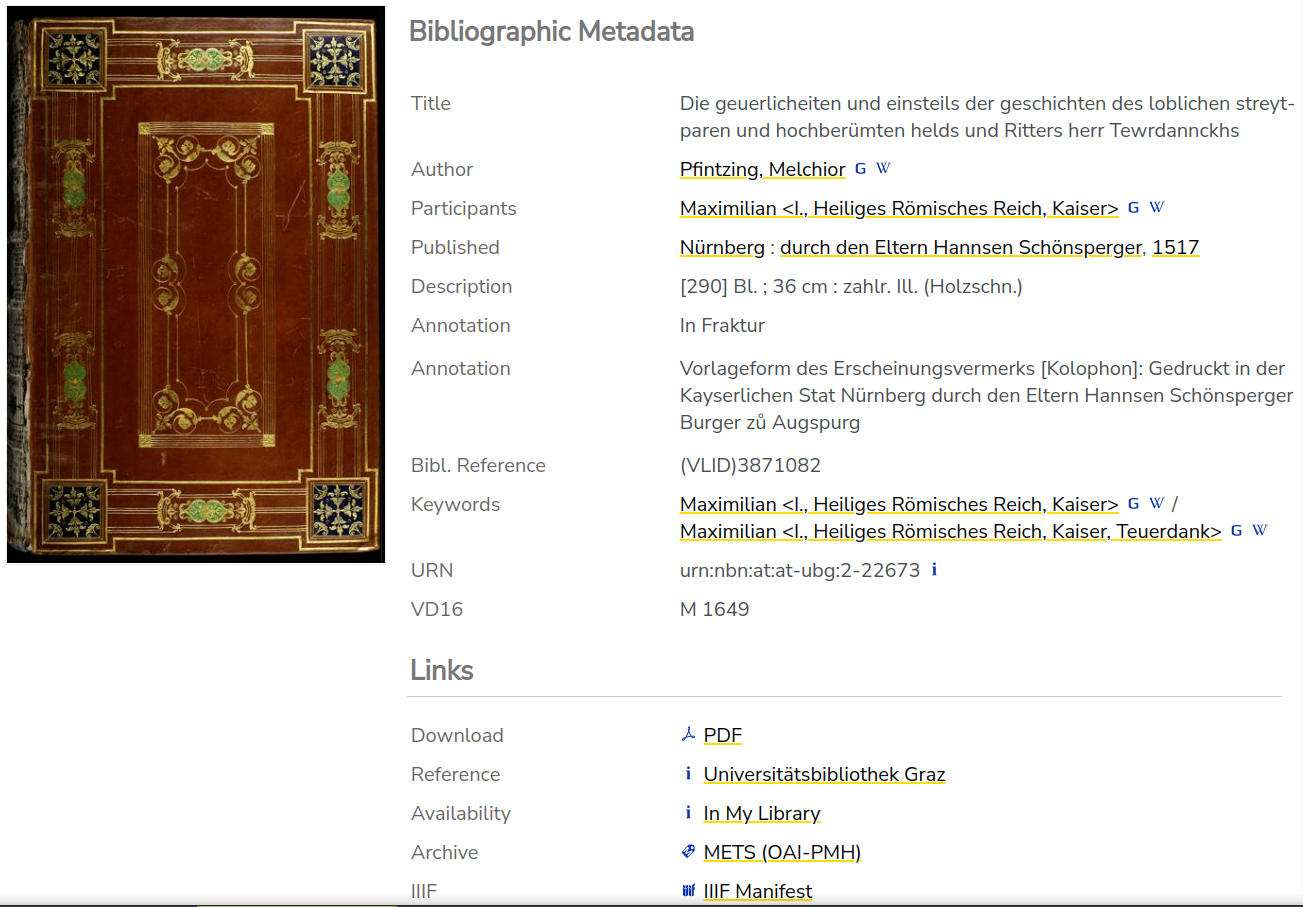
\includegraphics[width=0.95\textwidth]{img/theuerdank-biblio.png}
\end{frame}

%------------------------------------------------------------------------------
\begin{frame}[fragile,allowframebreaks]{MARC XML example}
    \footnotesize
    \href{https://lccn.loc.gov/2021667794/marcxml }{Library of Congress MARC XML for Theuerdank (simplified for demonstration purposes)}: \protect\url{https://www.loc.gov/item/2021667794}

    \begin{xmlcode}
<record xmlns="http://www.loc.gov/MARC21/slim" 
        xmlns:zs="http://docs.oasis-open.org/ns/search-ws/sruResponse">
    <leader>02892nam a22004093i 4500</leader>
    <controlfield tag="001">22061662</controlfield>

    <datafield ind1=" " ind2=" " tag="500">
      <subfield code="a">"BSB Shelfmark: Rar. 325 a"--Note extracted 
      from World Digital Library.</subfield>
    </datafield>
    
    <datafield ind1=" " ind2=" " tag="500">
      <subfield code="a">Original resource extent: 290 unnumbered 
      sheets : illustrations.</subfield>
    </datafield>
    [...]

</record>
\end{xmlcode}

    \begin{xmlcode}
<record xmlns="http://www.loc.gov/MARC21/slim" 
        xmlns:zs="http://docs.oasis-open.org/ns/search-ws/sruResponse">
        [...]
    
    <datafield ind1=" " ind2=" " tag="520">
      <subfield code="a">
      Among the many endeavors undertaken by the Holy Roman Emperor 
      Maximilian I (1459--1519) to further his legacy was his plan 
      of an epic retelling of his own life story in the form of 
      several works.       
      [...]
      Johann Schönsperger, a printer in Nuremberg, did the first, 
      very small print run in 1517, to be delivered to other princes 
      and sovereigns after the Emperor's death. 
      [...]
      Each of the 118 chapters is decorated by a xylograph 
      (wood engraving). The preparatory drawings for the xylographs 
      were created by the artists Leonhard Beck, 
      Hans Schäufelein, and Hans Burgkmair the Elder. The black-letter 
      type of the Theuerdank, designed by calligrapher Vinzenz Rockner, 
      was to become very influential for the development 
      of German typography.</subfield>
</datafield>

</record>
\end{xmlcode}

\end{frame}





% lead into XML and TEI


\section{Annotating with XML markup}


%-----------------------------------------------------
\begin{frame}{XML: eXtensible Markup Language}
\begin{columns}
\column{0.35\textwidth}
\begin{itemize}\small 
    \item \href{https://www.w3schools.com/xml/default.asp}{W3Schools Tutorial} 
    \item {paradigm of the separation of form and content} 
    \item {XML is a metalanguage}
\end{itemize}
\bgupper{w3schools}{black}{.xml} \\

\begin{itemize}\scriptsize 
    \item {RSS}, SOAP, XAML 
    \item {MathML}, {GraphML}~ 
    \item {XHTML}~
    \item {RDF}~
    \item {KML}~ 
    \item {Scalable Vector Graphics (SVG)}
\end{itemize}

\column{0.65\textwidth}
\metroset{block=fill}
\begin{block}{}
\begin{quote}
    \textbf{Extensible Markup Language (XML)} is a \textbf{markup language} and file format for storing, transmitting, and reconstructing arbitrary data. It defines a \textbf{set of rules for encoding documents} in a format that is \textbf{both human-readable and machine-readable.}  (\href{https://en.wikipedia.org/wiki/XML}{Wikipedia})
\end{quote}
\end{block}
\end{columns}

\end{frame}


%----------------------------------

\begin{frame}[fragile]{XML rules}
\begin{columns}
\column{0.42\textwidth}
\small
XML can be checked for \textbf{validity} (validation if it complies with a standard) and \textbf{well-formedness} (following the rules of XML) $\to$ will only be parsed if well-formed. Thus: \alert{Heed thy error messages!}\smallskip

There are rules on how elements can be named (you can look them up if relevant or will get informed by an error message). 

\bigskip

%
\includegraphics[width=0.1\textwidth]{doppelkeks.jpg}~\bg{alert}{white}{Doppelkeks} ~ ~\bg{alert}{white}{russische Puppe}~
\includegraphics[width=0.15\textwidth]{matroschka.jpg}\vspace{1em}

\mycommand{<key>value</key>}{XML as a key value notation} 
\column{0.55\textwidth}\footnotesize
\metroset{block=fill}
\begin{block}{Rules}
\begin{itemize}
    \item Hierarchical nesting below the root
    \item exactly one root element, i.e. one out-most russion doll
    \item start and end tag 
    \item tag names are case-sensitive (!) 
    \item empty elements allowed (\& can be shortened) 
\end{itemize}
\end{block}
\bigskip 

\begin{block}{Minimal example}
\begin{xmlcode}
<?xml version="1.0" ?>
<root>
  <element attribute="value">
    content
  </element>
  <!-- comment -->
</root>
\end{xmlcode}
\end{block}
\end{columns}

\end{frame}


%----------------------------------


\begin{frame}[fragile,allowframebreaks]{XML rules}

\small

\bg{w3schools}{white}{Prolog}~ \\
\mycommand{<xml version="1.0" encoding="utf-8">}{XML declaration}
\mycommand{<?xsl-stylesheet type="text/xsl" href="my.xsl"?>}{processing instructions  (optional)}
\bigskip

you can include document models (optional) \\
DTD, XML Schema, RelaxNG, Schematron 
\bigskip

\bg{w3schools}{white}{entities}~ `protected' characters that have a meta meaning in XML like: \\
\mycommand{&lt;}{<}
\mycommand{&gt;}{>}
\mycommand{&amp;}{\&}


\end{frame}


%-----------------
\begin{frame}{XML family and vocabularies}
\begin{columns}
\column{0.45\textwidth}
\footnotesize
\bg{w3schools}{white}{XML}~structured description of data \\
\bg{w3schools}{white}{XPath}~navigating xml documents \\
\bg{w3schools}{white}{XML Schema}~strict data model \\
\bg{w3schools}{white}{XSL}~Extensible Stylesheet Language  \\
\bg{w3schools}{white}{XSLT}~XSL-Transformations, i.e. transforming XML documents  \\
\bg{w3schools}{white}{XSL-FO}~ formatted output (e.g. print) \\
\bg{w3schools}{white}{XQuery}~query language for XML databases \\
\bg{w3schools}{white}{and more}~
\column{0.45\textwidth}
\metroset{block=fill}
\begin{block}{}
\footnotesize
\begin{itemize}
    \item \textbf{(X)HTML} Hypertext Markup Language 
    \item \textbf{EAD} Encoded Archival Description 
    \item \textbf{TEI} Text Encoding Initiative 
    \item \textbf{CEI} Charters Encoding Initiative 
    \item \textbf{MEI} Music Encoding Initiative 
    \item \textbf{LIDO} Lightweight Information Describing Objects (describing museum or collection objects)
    \item \textbf{SVG} Scalable Vector Graphics 
    \item \textbf{KML} Keyhole Markup Language (geography)
    \item \textbf{MathML} 
    \item \textbf{CML} Chemical Markup Language, \dots
\end{itemize}
\end{block}
\end{columns}


\end{frame}


%------------------------------------------------------------------------------

\begin{frame}[standout]
  \alert{Practice!} \\
  \normalsize
  Open a new XML document in your editor (Oxygen). \\
  Create new elements and find 3 ways to break it so that you get an error. \\
  Then fix the error.

\end{frame}



\begin{frame}[allowframebreaks]{Teaser: Digital editions -- some examples}

    \href{http://gams.uni-graz.at/o:ufbas.1563\#Eintrag-149}{GAMS ufbas}

    
\includegraphics[width=0.48\textwidth]{img/ufbas1.png}
    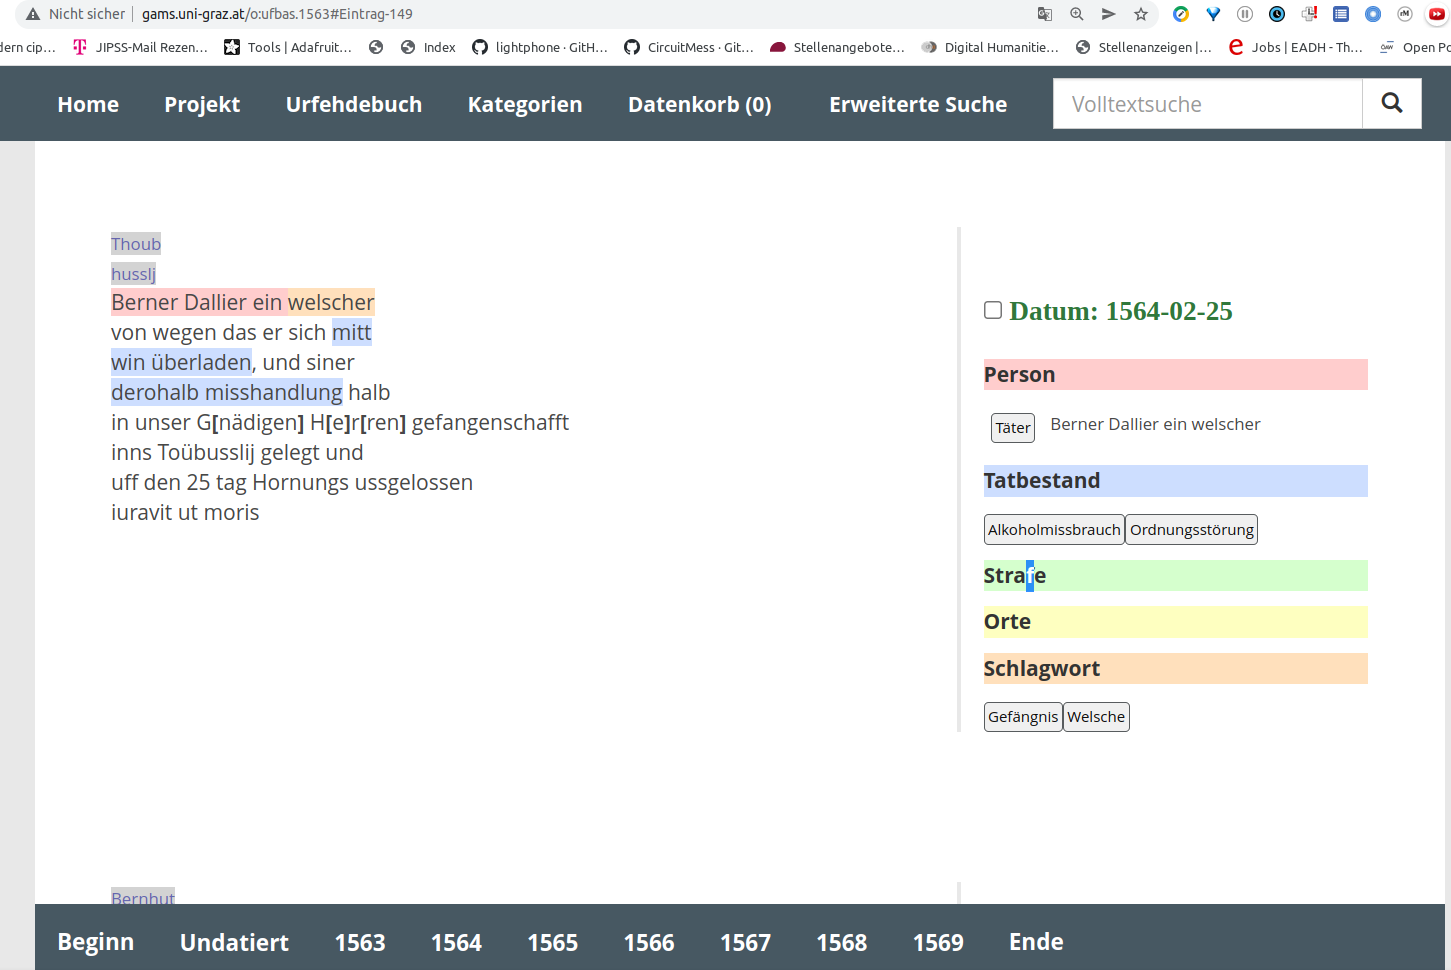
\includegraphics[width=0.48\textwidth]{img/ufbas2.png}
    
    \framebreak
    
    \href{https://gams.uni-graz.at/o:corema.pa1.recipes}{CoReMA} $\to$
    Look at: \protect\url{http://gams.uni-graz.at/corema}
    
    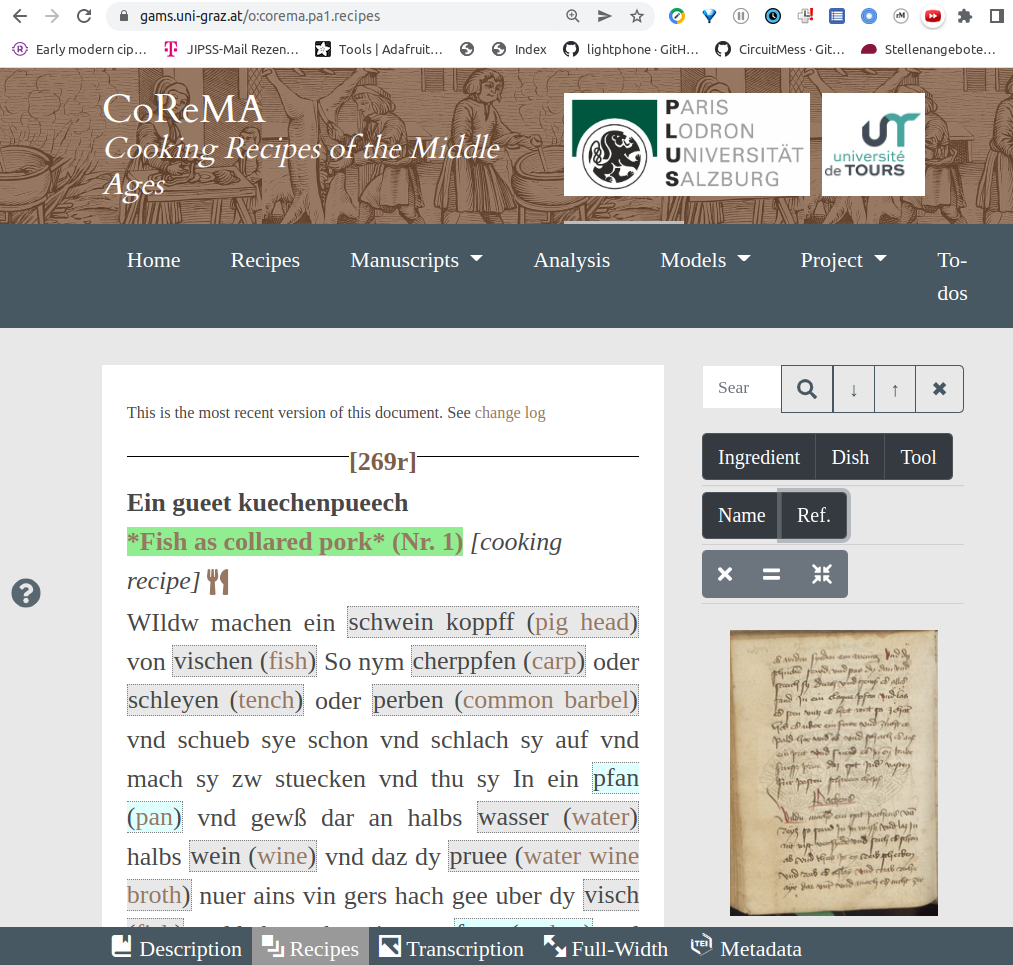
\includegraphics[width=0.6\textwidth]{img/corema-b1.png}
    
    \framebreak
    
    \href{https://furnaceandfugue.org}{Furnace and Fugue} (music in MEI, text and images)
    \begin{columns}
    \column{0.63\textwidth}
    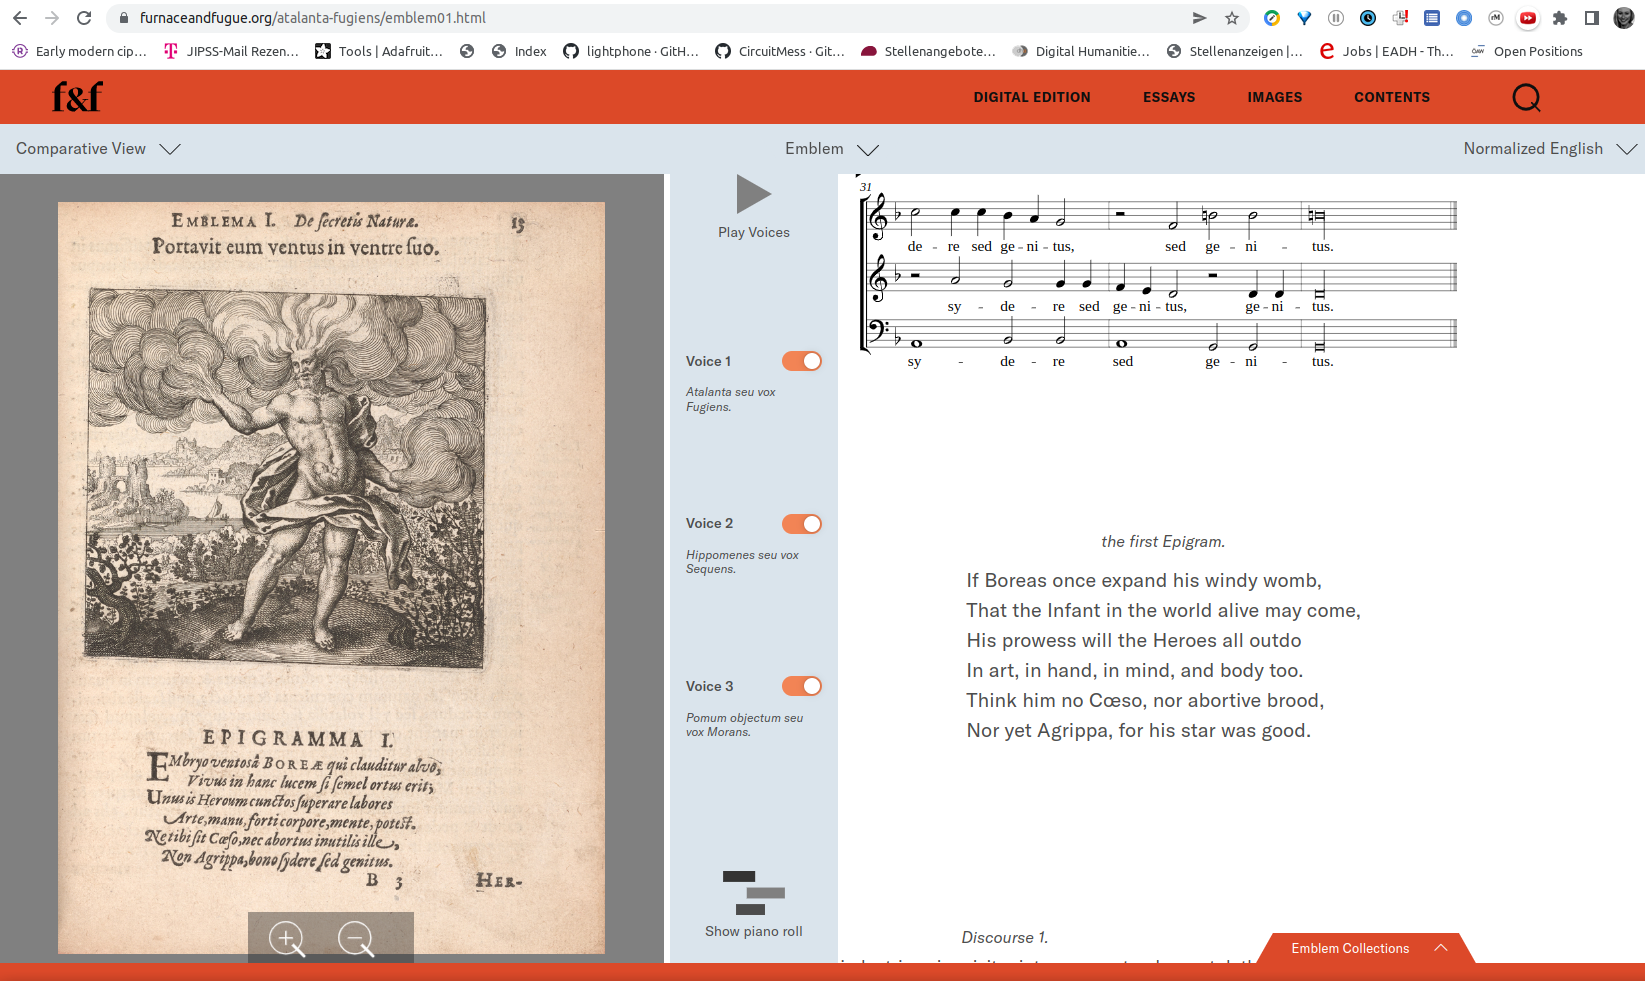
\includegraphics[width=\textwidth]{img/fnf1.png}
    \column{0.33\textwidth}
    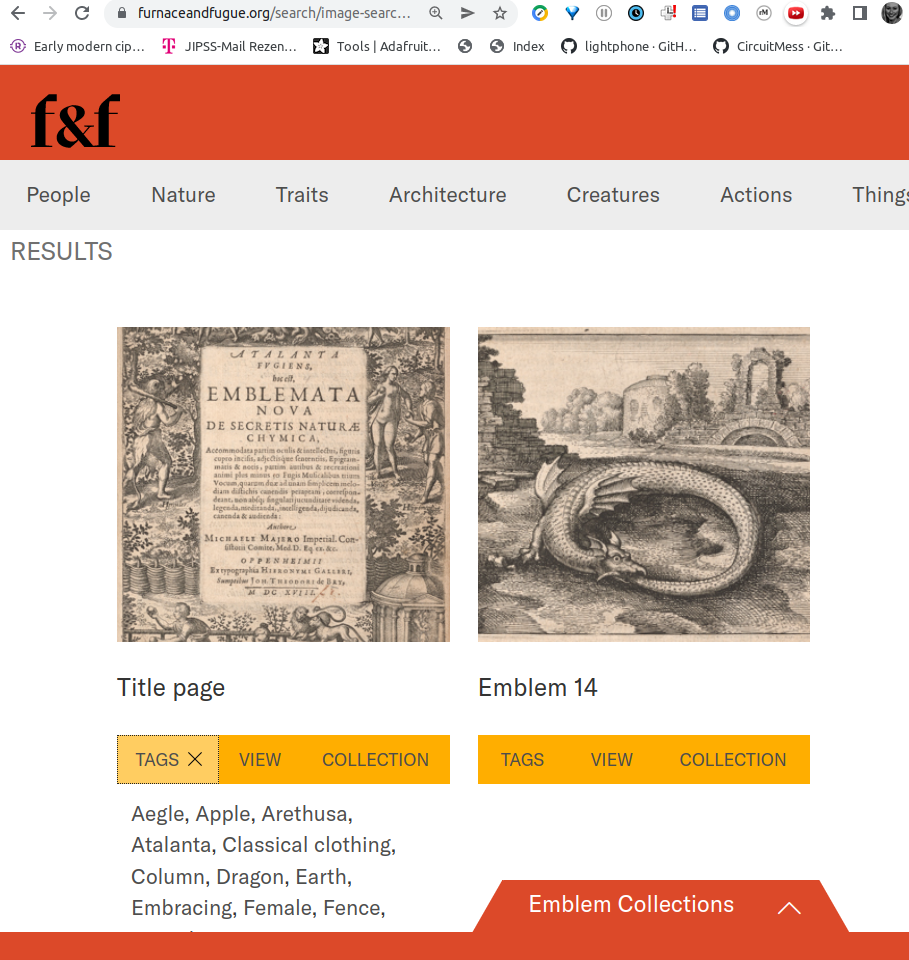
\includegraphics[width=\textwidth]{img/fnf2.png}
    \end{columns}
    
    
\end{frame}

%--------------------------------------------

\begin{frame}{From TEI to Edition}
What did all those examples have in common?
    \begin{itemize}\footnotesize
        \item all are digital editions
        \item all are based on data in TEI-XML
    \end{itemize}

That's what we want. -- How do we get there?

\metroset{block=fill}
\begin{block}{Remember}
\begin{itemize}\footnotesize
    \item XML is great for capturing \& long-term archiving data in its whole complexity
    \begin{itemize}
        \item[$\to$] \dots but also ends up chaotic with a lot of detail
        \item[$\to$] theoretically human-readable
        \item[$\to$] in practice, it's better to create a new representation of the data to read
    \end{itemize}
    \item \textbf{Desired result: }view/presentation, visualization and interaction with the data as a website (i.e. HTML data)
    \item \alert{$\to$ we need to transform the data}
\end{itemize}
\end{block}

\end{frame}

%--------------------------------------------


\begin{frame}{TEI Publication Tools}
There is a plethora of out-of-the-box solutions to make editions out of TEI data. 
$\to$
\alert{\href{https://wiki.tei-c.org/index.php/Category:Publishing_and_delivery_tools}{TEI List of Resources for Publishing and Delivery Tools}}, for example:
\begin{enumerate}
    \item teiPublisher
    \item EVT
    \item TEICHI
    \item Versioning Machine
    \item Boilerplate
    \item Oxgarage
    \item GAMS \dots 
\end{enumerate}

\end{frame}

%--------------------------------------------

\begin{frame}[allowframebreaks]{TEI Publisher: The Instant Publishing Toolbox}
    \begin{itemize}
        \item \protect\url{https://teipublisher.com/index.html}
        \item \protect\url{https://wiki.tei-c.org/index.php/TEI_Publisher}
        \item \protect\url{https://wiki.tei-c.org/index.php/TeiPublisher}
        \item \protect\url{http://hisoma.huma-num.fr/exist/apps/tei-publisher/index.html}
        \item ``Testimonial'': \href{https://digitalintellectuals.hypotheses.org/3912}{Florian Chiffoleau (2020), Blog Post: \emph{Publication of my digital edition -- Working with TEI Publisher.}}
    \end{itemize}
    
    
\includegraphics[width=0.7\textwidth]{img/tei-publisher1.png}
    
    \framebreak
    
    Demos:  \href{https://teipublisher.com/exist/apps/vangogh/let001.xml}{Van Gogh Letters} \sep \href{https://teipublisher.com/exist/apps/eebo/index.html}{Early English Books Online (EEBO)}
    
    \begin{columns}
    \column{0.33\textwidth}
    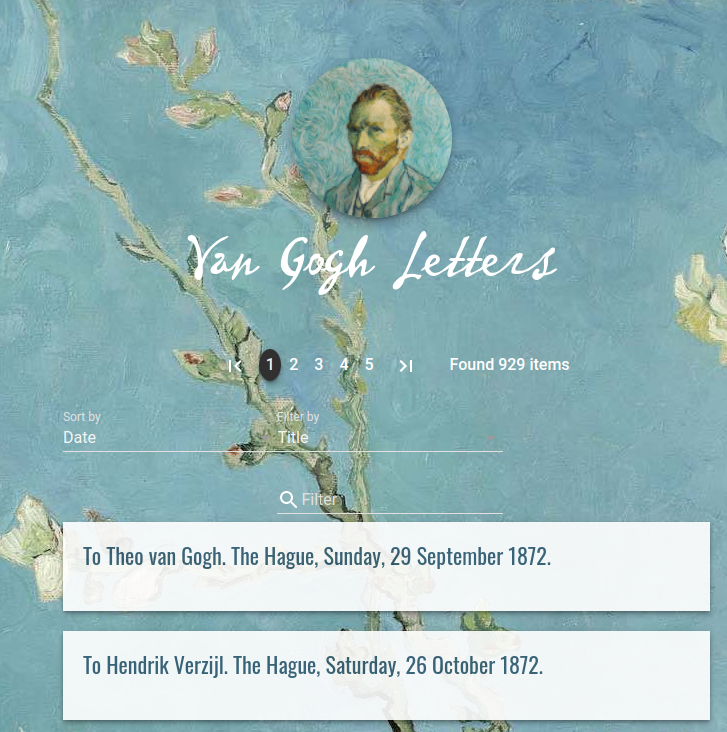
\includegraphics[width=\textwidth]{img/tei-publisher2.png}
    \column{0.33\textwidth}
    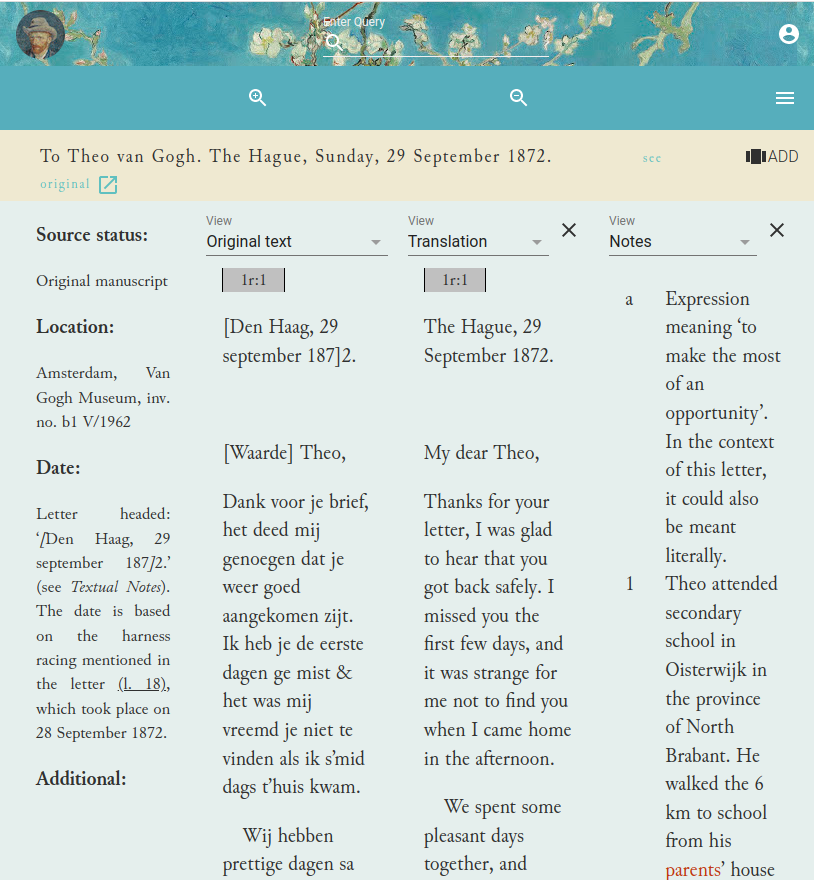
\includegraphics[width=\textwidth]{img/tei-publisher3.png}
    \column{0.33\textwidth}
    
\includegraphics[width=\textwidth]{img/tei-publisher4.png}
    \end{columns}
\end{frame}


%--------------------------------------------

\begin{frame}{Edition Visualization Technology (EVT)}

\begin{columns}
\column{0.53\textwidth}
\begin{itemize}\scriptsize
    \item \protect\url{http://evt.labcd.unipi.it/} -- \protect\url{http://evt-project.sourceforge.net/}
    \item \protect\url{https://visualizationtechnology.wordpress.com/}
    \item Roberto Rosselli Del Turco, Giancarlo Buomprisco, Chiara Di Pietro, Julia Kenny, Raffaele Masotti and Jacopo Pugliese: \emph{Edition Visualization Technology: A Simple Tool to Visualize TEI-based Digital Editions}, Journal of the Text Encoding Initiative 8 (2014/15): Selected Papers from the 2013 TEI Conference “TEI Processing: Workflows and Tools”; \protect\url{https://doi.org/10.4000/jtei.1077}
    \item Del Turco, Roberto Rosselli. “Designing an Advanced Software Tool for Digital Scholarly Editions: The Inception and Development of EVT (Edition Visualization Technology).” \emph{Textual Cultures}, vol. 12, no. 2, 2019, pp. 91–111. JSTOR, \protect\url{www.jstor.org/stable/26821538}. 
\end{itemize}
\column{0.45\textwidth}
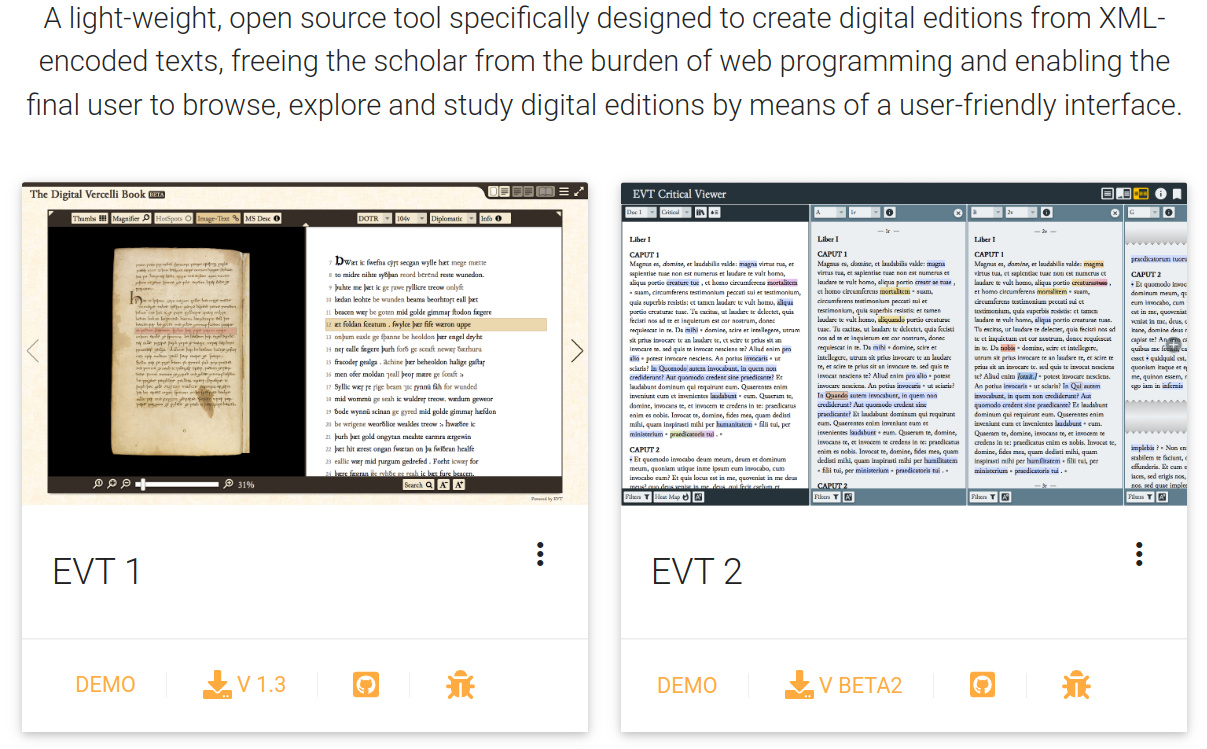
\includegraphics[width=\textwidth]{img/evt-example.png}
\end{columns}



\end{frame}

%--------------------------------------------

\begin{frame}{TeiCHI – Bringing TEI Lite to Drupal}


\begin{columns}
\column{0.38\textwidth}
\begin{itemize}\scriptsize
    \item TEIChi: a TEI lite integration into Drupal (\protect\url{http://teichi.org})
    \item Sebastian Pape, Christof Schöch and Lutz Wegner: \emph{TEICHI and the Tools Paradox. Developing a Publishing Framework for Digital Editions}, Journal of the Text Encoding Initiative 2 (2012): Selected Papers from the 2010 TEI Conference; \protect\url{https://doi.org/10.4000/jtei.432}
    \item \href{https://wiki.tei-c.org/index.php/TEICHI}{TEICHI wiki}
\end{itemize}
\column{0.68\textwidth}
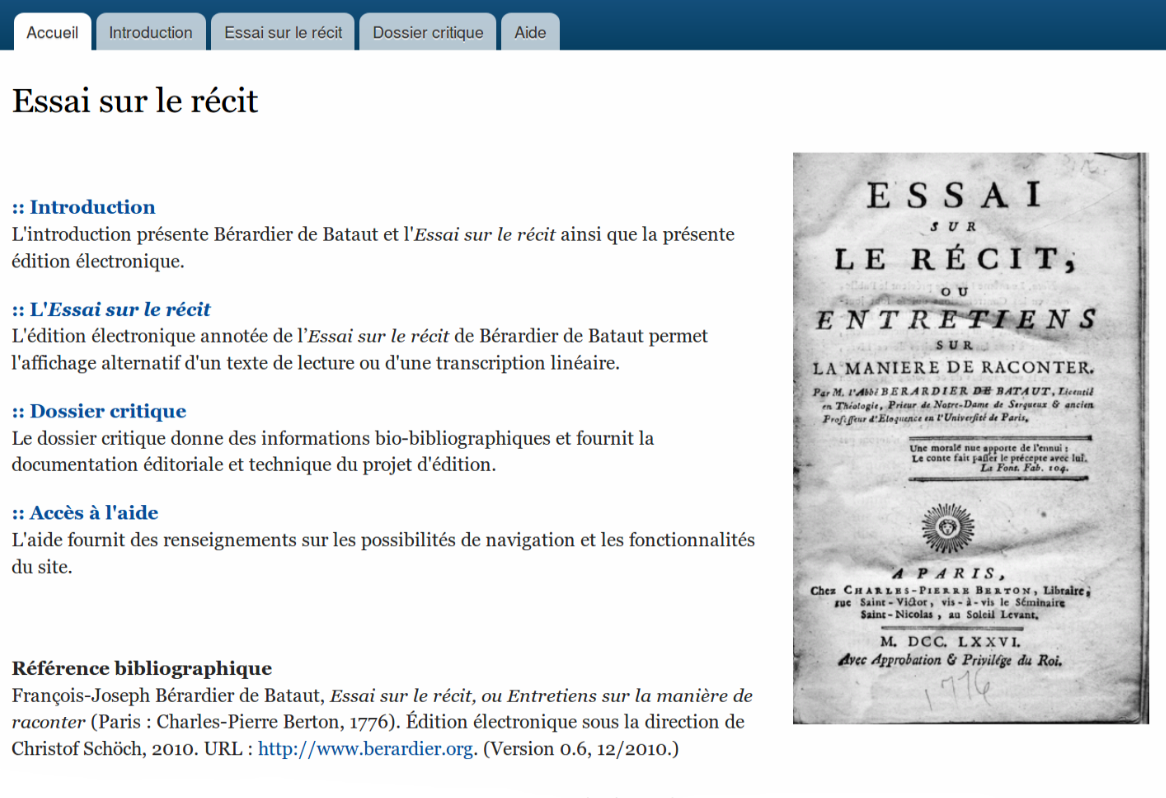
\includegraphics[width=\textwidth]{img/teichi-example.png}
\end{columns}



\end{frame}

%--------------------------------------------

\begin{frame}{The Versioning Machine}

\begin{itemize}\small
    \item Versioning Machine (\protect\url{http://v-machine.org/})
    \item \href{https://tei-c.org/activities/projects/the-versioning-machine}{The TEI Versioning Machine}
    \href{https://digitalhumanities.duke.edu/tools/versioning-machine}{Versioning Machine (Duke)}
\end{itemize}

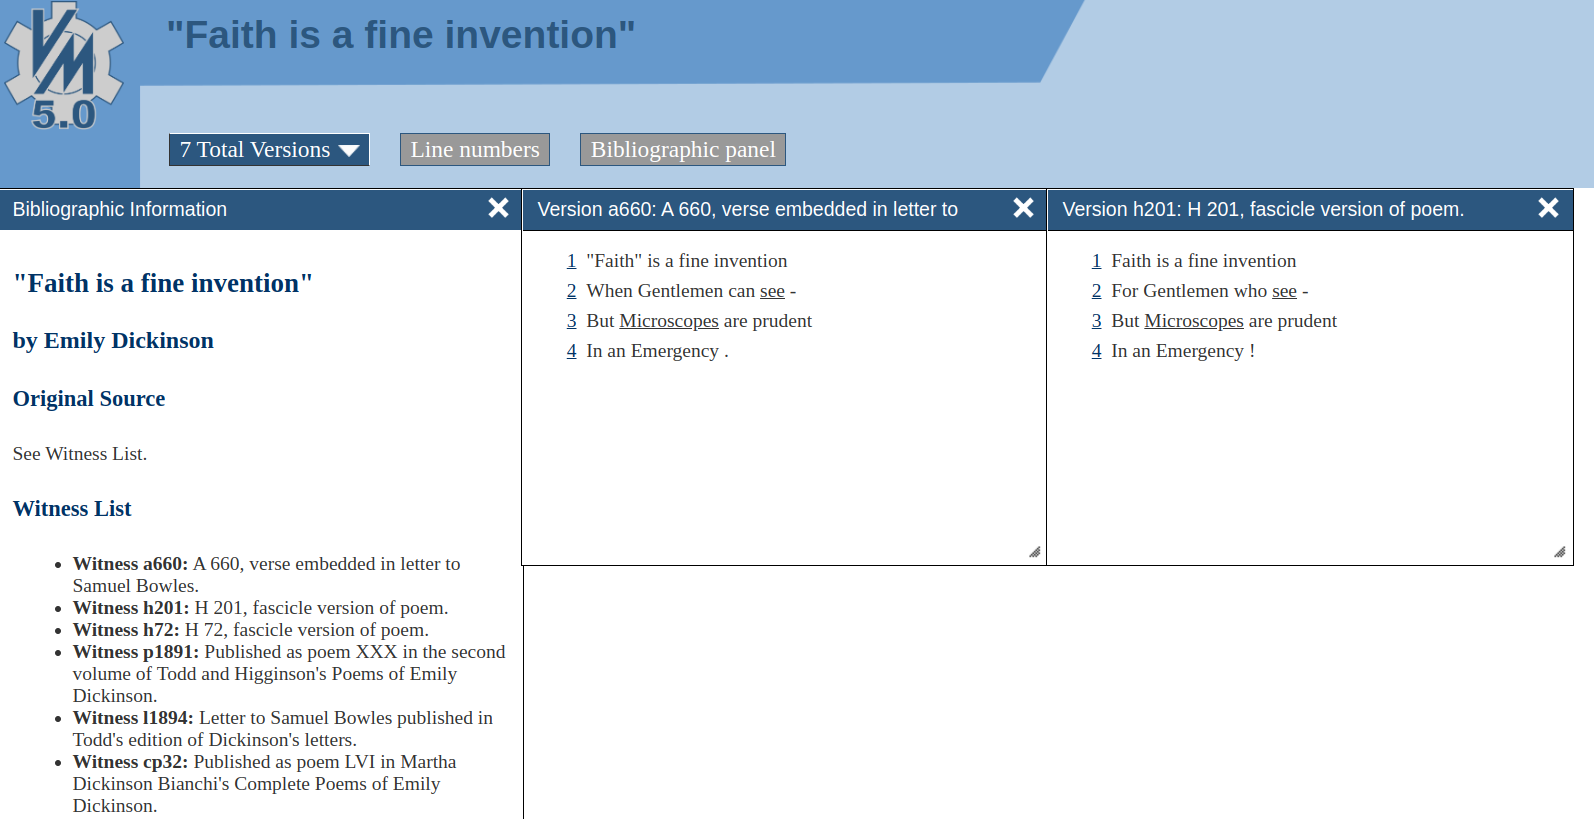
\includegraphics[width=0.9\textwidth]{img/tei-versioning-machine.png}

\end{frame}

%--------------------------------------------

\begin{frame}{TEI Boilerplate}

\begin{columns}
\column{0.48\textwidth}
\begin{itemize}\footnotesize
    \item \protect\url{http://teiboilerplate.org/}
    \item Boilerplate (\protect\url{http://dcl.slis.indiana.edu/teibp/})
    \item \href{http://dcl.slis.indiana.edu/teibp/content/demo.xml}{Demo}
    \item \href{https://wiki.tei-c.org/index.php/TEI_Boilerplate}{TEI Boilerplate Wiki}
    \item \href{https://www.i-d-e.de/wp-content/uploads/2014/07/boilerplate.pdf}{Slides on TEI Boilerplate}
    \item \href{http://tei.it.ox.ac.uk/Talks/2015-07-dhoxss/ex-boilerplate.pdf}{Exercise on TEI Boilerplate}
    \item \href{http://journalofdigitalhumanities.org/2-3/tei-boilerplate}{Poster on TEI Boilerplate}
\end{itemize}

\column{0.48\textwidth}
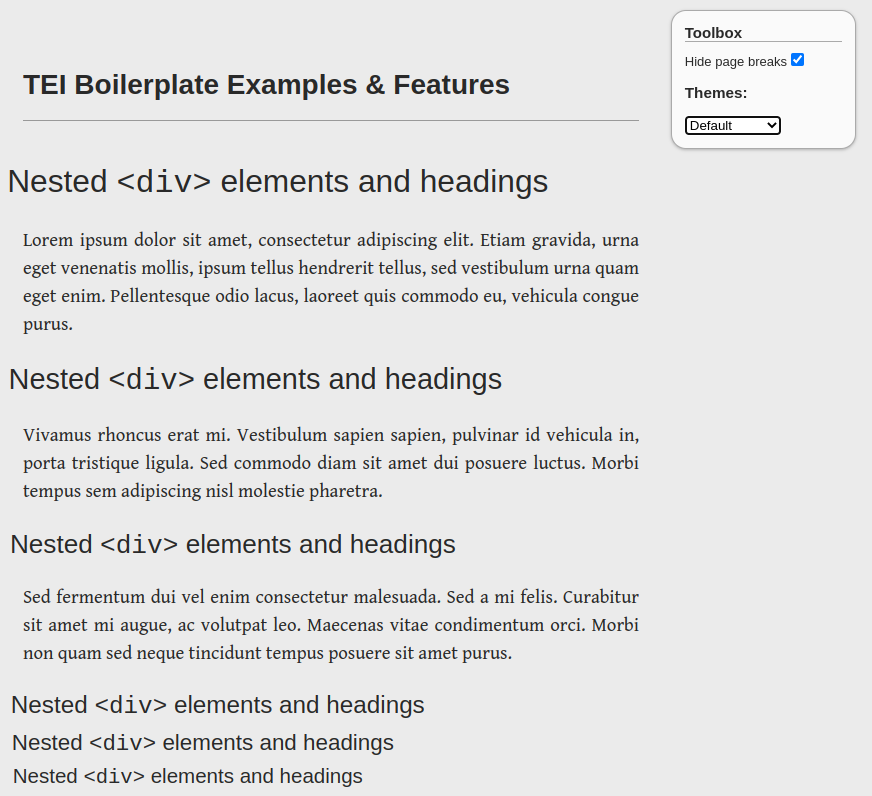
\includegraphics[width=\textwidth]{img/tei-boilerplate-example.png}
\end{columns}

\end{frame}

%--------------------------------------------

\begin{frame}{Oxgarage}
\metroset{block=fill}\footnotesize

\begin{columns}
\column{0.48\textwidth}
\begin{itemize}
    \item REST-based transformation web service for TEI documents (\protect\url{https://oxgarage.tei-c.org/})
    \item allows you to transform a number of (markup-based) formats to TEI or create them from TEI (\texttt{.html}, \texttt{.tex}, \texttt{.docx}, \dots)
    \item \href{https://tei-c.org/Vault/P5/3.6.0/doc/tei-xsl}{Based on TEI base stylesheets} (\protect\url{http://www.tei-c.org/Tools/Stylesheets/})
    \item[\textcolor{w3schools}{\faCheck}] very useful tool
    \item[\textcolor{alert}{\faClose}] not all TEI elements taken into account, not customizable
\end{itemize}
\column{0.48\textwidth}
\begin{block}{Oxgarage}
\dots offers a set of standard stylesheets to convert between TEI-encoded XML documents and other documents, mostly markup-based, such as \texttt{.docx}, \texttt{.html} or \texttt{.tex}. 

However, not all elements are covered and you have no control over how exactly they are processed. 
\end{block}
\end{columns}\medskip

Tools make things easier superficially but can come at a cost: potential bugs, less than ideal usability, lack of control and customizability:

\alert{$\to$ to customize we need to write our own transformation using XSL stylesheets}


\end{frame}



%--------------------------------------------

\begin{frame}[allowframebreaks]{GAMS (Humanities Asset Management System)}
\metroset{block=fill}
    \begin{columns}
    \column{0.44\textwidth}
    \begin{itemize}\small
        \item GAMS (\emph{Geisteswissenschaftliches Asset Management System} = AMS for the Humanities)
        \item based on \textbf{FEDORA} (\emph{Flexible Extensible Digital Object Repository Architecture}) = infrastructure dedicated to the persistent archival and management of resources considered to be worthy of long-term preservation.
    \end{itemize}
    \column{0.55\textwidth}
    
\includegraphics[width=\textwidth]{img/gams.png}
    \end{columns}
    \bigskip 
    
    \protect\url{https://gams.uni-graz.at}
    
    \framebreak
    
    \begin{columns}
    \column{0.58\textwidth}
    \begin{itemize}\small
        \item user access provided through the \textbf{Cirilo client}
        \item \textbf{functionalities:} object creation and management, versioning, normalization \& standards, choice of data formats.
        \item offers a plethora of \textbf{pre-defined content models} for data such as TEI, MEI, LIDO, SKOS, ontologies, R code and story lines
        \item $\to$ offers publication pipelines but is highly customizable
        \item more info: \protect\url{http://gams.uni-graz.at/doku}
    \end{itemize}
    \column{0.48\textwidth}
    
\includegraphics[width=\textwidth]{img/gams.png}
    \end{columns}
\end{frame}



%--------------------------------------------

\begin{frame}[allowframebreaks]{Long-term archiving heritage data}
\metroset{block=fill}
    \begin{columns}
    \column{0.4\textwidth}
    \begin{block}{Long-term preservation} denotes the process of maintaining, curating and keeping data usable over a long period of time (10+~years).
    \end{block}
    \column{0.58\textwidth}
    \begin{block}{Key functionalities of long-term archiving architectures include}
    \begin{itemize}\footnotesize
        \item persistent identification, 
        \item versioning, 
        \item support of different data formats, 
        \item management of associated metadata, 
        \item data export and retrieval, 
        \item security and scalability. 
    \end{itemize}
    
    Special emphasis is placed on 
    \begin{itemize}\footnotesize
        \item sustainability,
        \item citability \& 
        \item guarantee of long-term access to the contained resources. 
    \end{itemize}
    \end{block}
    \end{columns}
    
    \begin{block}{XML is great for long-term archiving!}
        Consequently, data formats and software used for preservation should follow \textbf{open source \& non-proprietary standards}; data is ideally encoded in an \textbf{unicode XML format}:
        \begin{itemize}
            \item plain text files are small
            \item human- \& machine-readable
            \item recognized standard stable since 1998
            \item more on XML later\dots
        \end{itemize}
    \end{block}
    
 \end{frame}



%--------------------------------------------

\begin{frame}[allowframebreaks]{Examples of data quality in GAMS}   
\metroset{block=fill}
    \begin{columns}
    \column{0.56\textwidth}
    
\includegraphics[width=\textwidth]{img/ufbas1.png}
    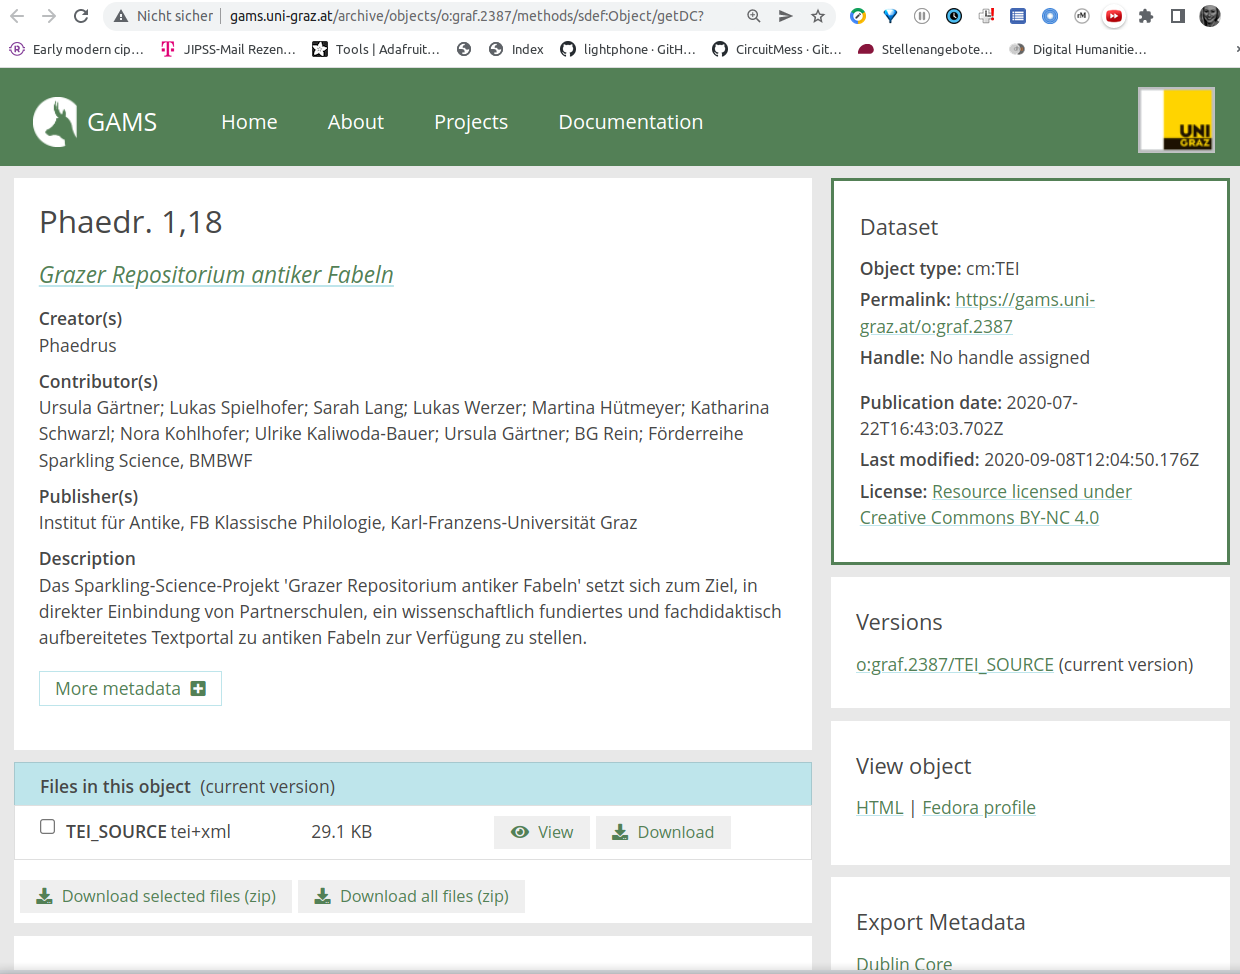
\includegraphics[width=\textwidth]{img/gams-graf-dc-metadata.png}
    \column{0.4\textwidth}
    \small
     $\leftarrow$ {\footnotesize \protect\url{http://gams.uni-graz.at/o:ufbas.1563}}
    \bigskip
    
    \begin{itemize}
        \item \textbf{top image:} info on recommended citation, downloadable source data in XML \& RDF
        \item \textbf{below:} `data view' of the Dublin Core (DC) metadata for an XML object in GAMS (ensuring citability, etc.)
    \end{itemize}
    \bigskip 
    
    $\leftarrow$ {\scriptsize \protect\url{http://gams.uni-graz.at/archive/objects/o:graf.2387/methods/sdef:Object/getDC?}}
    \end{columns}
    
    \begin{itemize}
        \item GAMS isn't an out-of-the-box tool -- it's something between a \textbf{Content Management System (CMS)}, a \textbf{repository} (long-term archiving) and a \textbf{publication platform}. 
        \item The XSLT transformations applied to files in GAMS are custom but there are \textbf{wippets} (standard javascript functionalities $\to$ \emph{widget + snippet}, \href{https://github.com/KONDE-AT/gams-wippets}{example here}) and \textbf{standard templates} which can be reused. 
        \item as a publication platform: presentation and long-term archiving, allowing for persistent access to the data, versioning, etc.
    \end{itemize}
    
    One more example: \protect\url{https://gams.uni-graz.at/beurb}
    \bigskip
    
    \begin{columns}
    \column{0.5\textwidth}
    
   \begin{block}{Metadata view on XML data}
    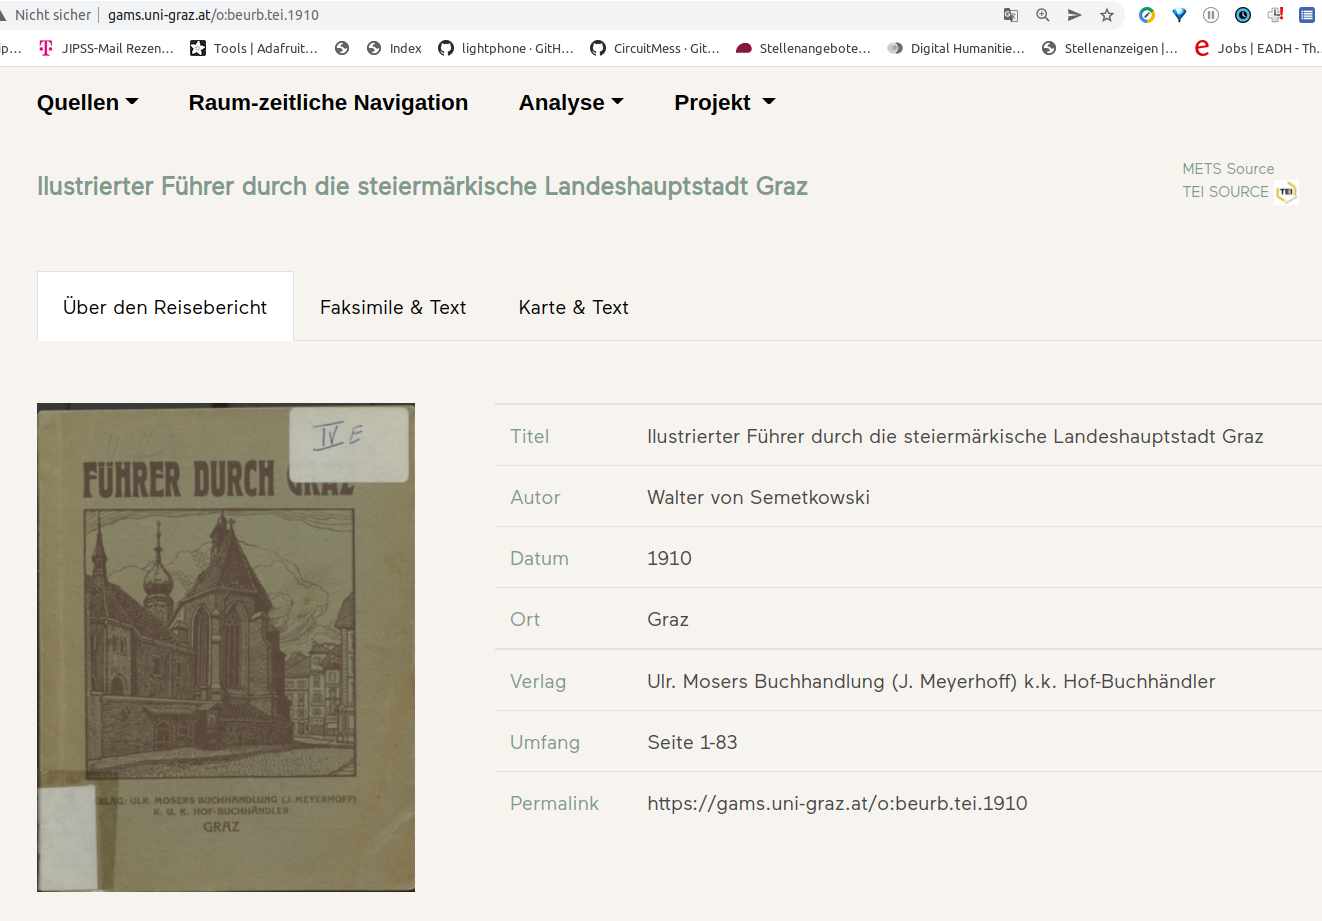
\includegraphics[width=\textwidth]{img/gams-beurb1.png}
   \end{block}
    \column{0.5\textwidth}
    \begin{block}{Map view linked to edited text} 
    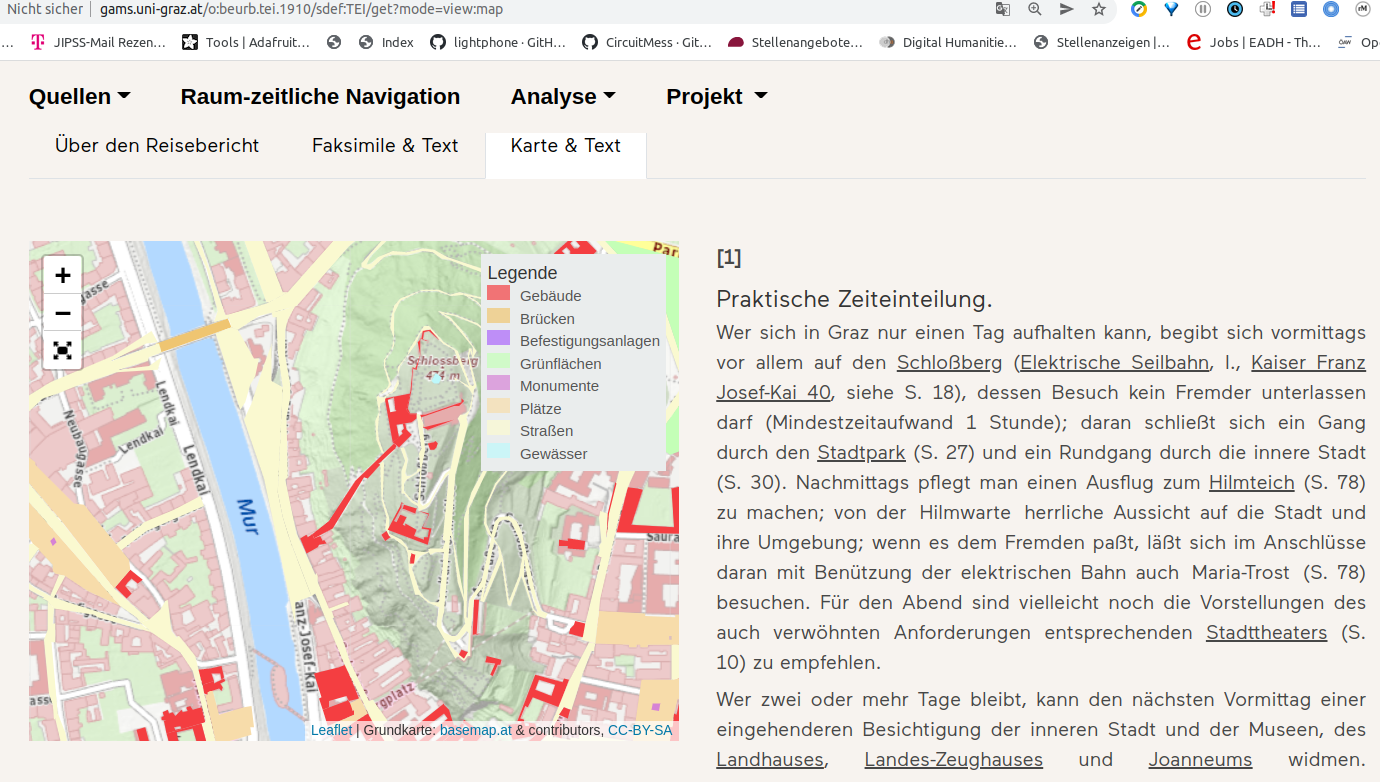
\includegraphics[width=\textwidth]{img/gams-beurb2.png}
    \end{block}
    \end{columns}
    Both views are created `on-the-fly' from the same XML file (=\emph{single source principle}, more on that later\dots).
\end{frame}


%-----------------------------------------------------



\begin{frame}[standout]

  \alert{Practice!}
  
  \normalsize
  Use \alert{\protect\url{https://oxgarage.tei-c.org/}} to transform some data to HTML. What do you notice? Do you like it or would you need to customize?
\end{frame}







\section{Text Encoding Initiative}
%-----------------------------------------------------
\begin{frame}[fragile]{TEI Primer}
\footnotesize\metroset{block=fill}

\begin{columns}
\column{0.48\textwidth}
\bg{alert}{white}{Text Encoding Initiative}\\
\bgupper{w3schools}{black}{.xml}\\
XML-Standard, i.e. convention on how to use XML so that resulting data will be interoperable between different projects.

(founded in 1987, consortium since 2000)

\begin{block}{}
\begin{quote}
    The Text Encoding Initiative (TEI) is a text-centric community of practice in the academic field of digital humanities, operating continuously since the 1980s. The community currently runs a mailing list, meetings and conference series, and maintains the TEI technical standard, a journal, a wiki, a GitHub repository and a toolchain. (\href{https://en.wikipedia.org/wiki/Text_Encoding_Initiative}{Wikipedia})
\end{quote}
\end{block}

\column{0.48\textwidth}
\begin{block}{TEI minimal example}
\begin{xmlcode}
<TEI> <!-- root element -->
    <teiHeader> 
      <!-- author, title, dating, 
           sources, edition rules, etc. -->
    </teiHeader> 
    <text> ... </text>
</TEI>
\end{xmlcode}
\end{block}

\begin{block}{Resources}
    \begin{itemize}\scriptsize
        \item \href{http://www.tei-c.org/Support/Learn/}{Learn TEI} 
        \item \href{http://www.tei-c.org/support/learn/teach-yourself-tei/}{Teach Yourself} \item P5 = 5. Proposal 
        \item MEI for music 
        \item CEI for charters 
        \item \href{http://www.tei-c.org/}{http://www.tei-c.org/} 
    \end{itemize}
\end{block}
\end{columns}

\end{frame}

%-------------------------------------
\begin{frame}[fragile]{TEI Header}
\footnotesize
\bg{alert}{white}{fileDesc}~ = bibliographical description of the contents of the document  \\
\bg{alert}{white}{encodingDesc}~ = connection of electronic document to source (i.e. transcription rules, etc.)  \\

\begin{xmlcode}
<TEI> <!-- root element -->
    <teiHeader>
        <fileDesc> ... </fileDesc> <!-- obligatory --> 
        <encodingDesc> <!-- optional -->
        <profileDesc> <!-- optional -->
        <revisionDesc> <!-- optional -->
    </teiHeader> 
    <text> ... </text>
</TEI>
\end{xmlcode}

\bg{alert}{white}{profileDesc}~ = decribes all non-bibliogaphical aspects of the text (i.e. creation, languages) \\
\bg{alert}{white}{revisionDesc}~ = tracks changes in the digital document 
\end{frame}

%-----------------------------------
\begin{frame}[fragile,allowframebreaks]{Using TEI}
\footnotesize
\href{http://www.tei-c.org/release/doc/tei-p5-doc/en/html/SG.html}{Gentle Intro to XML}

\begin{multicols}{2}
\bg{alert}{white}{TEI Core}~ 
\begin{itemize}
    \item \textbf{div} (division) \item \textbf{p} (paragraph) \item \textbf{head} (heading) \item \textbf{lb} (linebreak) \item \textbf{pb} (page break / beginning) \item \textbf{hi} (highlight) \item \textbf{l} (line) \item \textbf{lg} (line group) \item \textbf{list} \item \textbf{item} \item \textbf{listBibl} \item \textbf{bibl} (bibliographical information)
\end{itemize}

\bg{alert}{white}{Attributes}~ 
\begin{itemize}
    \item \textbf{@n} (label) \item \textbf{@type} (typing) \item \textbf{xml:id} (unique identifier) \item \textbf{xml:lang} (language) \item \textbf{@rend} (rendering) \item \textbf{@ana} (interpretation)
\end{itemize}
\end{multicols}

\begin{xmlcode}
<foreign xml:lang="en">word</foreign>
<term type="homonym"/>
<date when="2009-04-27"/>
<time when="12:00:00"/>
<name type="person"/>
<persName n="Caesar" xml:id="#44BC">Caesaris</persName> 
<!-- or -->
<persName key="ID.01.208"/>
<person/>
<emph/> <hi rend="italic">italic text</hi>
<seg/> <abbr type="acronym"/>
<placeName xml:id="#Whitby">Abbey</placeName>
\end{xmlcode}

\framebreak

\bg{alert}{white}{Name spaces}~ identified via URI 

\bg{w3schools}{white}{<prefix:name>}~
e.g. \texttt{<tei:p>} (`I mean the \texttt{<p>} according to the TEI standard.') \\

\bg{alert}{white}{declaration}~ <element xmlns=“URI“> \dots \\
<prefix:element xmlns:prefix=“URI“> \dots \\
e.g. 
\begin{xmlcode}
<tei:p xmlns:tei=“http://www.tei-c.org/ns/1.0“>...
\end{xmlcode}


\end{frame}



\begin{frame}[fragile]{TEI is organized in modules}
\footnotesize
Acts of speech (\href{http://www.tei-c.org/release/doc/tei-p5-doc/en/html/examples-sp.html}{reference}) if speaker name is mentioned, otherwise  \href{http://www.tei-c.org/release/doc/tei-p5-doc/en/html/examples-said.html}{TEIs `said'}:
\begin{xmlcode}
<sp who="#person">
    <speaker>1.</speaker> <p>Bla, bla, bla.</p>
</sp>

<said who="#Adolphe">- Alors, Albert, quoi de neuf?</said>
\end{xmlcode}

Letters in TEI \href{http://www.tei-c.org/release/doc/tei-p5-doc/en/html/DS.html#DSOC}{(reference)}

\begin{xmlcode}
<div type="letter" n="14">
    <head>Letter XIV: Miss Clarissa Harlowe to Miss Howe</head>
        <opener>
            <dateline>Thursday evening, March 2.</dateline>
            <salute>Hallo,</salute>
        </opener>
    <p>On Hannah's depositing my long letter ...</p>
    <closer>
        <salute>Yours more than my own,</salute>
        <signed>Clarissa Harlowe</signed>
    </closer>
</div>
\end{xmlcode}
\end{frame}

%--------------------------------
\begin{frame}[fragile]{Names, Dates, Places}
\footnotesize
\bg{w3schools}{white}{\emph{Named Entities} \& indirect reference}\\
\href{http://www.tei-c.org/release/doc/tei-p5-doc/en/html/ND.html}{TEI 13: Names, Dates, People, Places} 

\metroset{block=fill}
\begin{columns}
\column{0.4\textwidth}
\begin{itemize}
    \item \textbf{persName} for personal names, \textbf{<rs>} for \emph{referring string} when mentioned indirectly (`he', `the woman', etc.) $\to $\textbf{@key} or \textbf{@ref} to specify who it is  (\href{http://www.tei-c.org/release/doc/tei-p5-doc/en/html/CO.html#CONARS}{reference}). \item \textbf{forename} 
    \item \textbf{surname} 
    \item \textbf{roleName} (z.B. `king') 
    \item  \textbf{genName} (`the Younger') 
    \item \textbf{addName} 
    \item \textbf{nameLink} (`von').
\end{itemize}

\column{0.58\textwidth}
\begin{xmlcode}
<name role="writer" type="person"
ref="http://d-nb.info/gnd/118540238">
Goethe</name>
<person>
  <addName type="Former">Murray</addName>
  <forename>Wilhelmina</forename>
  <addName type="nickname">Mina</addName>
</person>
\end{xmlcode}
\end{columns}

\end{frame}




%-----------------------------------------------------
\begin{frame}[fragile,allowframebreaks]{Metadata in the TEI Header}
\subsection{teiHeader, msDesc, sourceDesc, titlePage}
\small

\begin{xmlcode}
<teiHeader>
 <fileDesc>
  <titleStmt>
   <title>
<!-- title of the resource -->
   </title>
  </titleStmt>
  <publicationStmt>
   <p>
<!-- Information about distribution of the resource -->
   </p>
  </publicationStmt>
  <sourceDesc>
   <p>
<!-- Information about source from which the resource derives -->
   </p>
  </sourceDesc>
 </fileDesc>
</teiHeader>
\end{xmlcode}


The title and author in the \texttt{<titleStmt>} isn't the bibliographic data from the source! It describes the digital document and its authors or editors.

If you want to desribe your source documents, you need elements like \texttt{<sourceDesc>} or \texttt{<msDesc>}:
\begin{xmlcode}
<sourceDesc>
 <bibl>
  <title level="a">The Interesting story of the Children 
  in the Wood</title>. In
 <author>Victor E Neuberg</author>, <title>The Penny Histories</title>.
 <publisher>OUP</publisher>
  <date>1968</date>. </bibl>
</sourceDesc>
\end{xmlcode}

\begin{xmlcode}
<sourceDesc>
 <p>Born digital: no previous source exists.</p>
</sourceDesc>
\end{xmlcode}

\begin{xmlcode}
<teiHeader>
 <fileDesc>
  <titleStmt>
   <title>Thomas Paine: Common sense, a
       machine-readable transcript</title>
   <respStmt>
    <resp>compiled by</resp>
    <name>Jon K Adams</name>
   </respStmt>
  </titleStmt>
  <publicationStmt>
   <distributor>Oxford Text Archive</distributor>
  </publicationStmt>
  <sourceDesc>
   <bibl>The complete writings of Thomas Paine, collected and edited
       by Phillip S. Foner (New York, Citadel Press, 1945)</bibl>
  </sourceDesc>
 </fileDesc>
</teiHeader>
\end{xmlcode}

\end{frame}

%-----------------------------------------------------
\begin{frame}[fragile]{\texttt{<msDesc>}}

\begin{xmlcode}
<msDesc>
 <msIdentifier>
  <settlement>Oxford</settlement>
  <repository>Bodleian Library</repository>
  <idno type="Bod">MS Poet. Rawl. D. 169.</idno>
 </msIdentifier>
 <msContents>
  <msItem>
   <author>Geoffrey Chaucer</author>
   <title>The Canterbury Tales</title>
  </msItem>
 </msContents>
 <physDesc>
  <objectDesc>
   <p>A parchment codex of 136 folios, measuring approx
       28 by 19 inches, and containing 24 quires.</p>
   <p>The pages are margined and ruled throughout.</p>
   <p>Four hands have been identified in the manuscript: the first 44
       folios being written in two cursive anglicana scripts, while the
       remainder is for the most part in a mixed secretary hand.</p>
  </objectDesc>
 </physDesc>
</msDesc>
\end{xmlcode}

$\to$ Use websearch (`tei msDesc') to learn how to use new elements (\href{https://tei-c.org/release/doc/tei-p5-doc/en/html/ref-msDesc.html}{overview} and find \href{https://tei-c.org/release/doc/tei-p5-doc/en/html/examples-msDesc.html}{examples like this}).

\end{frame}




%-----------------------------------------------------
\begin{frame}[fragile]{\texttt{<titlePage>}}

To describe a title page (e.g. early modern print copperplates, etc.), use \texttt{<titlePage>}:
\begin{xmlcode}
<titlePage>
 <docTitle>
  <titlePart type="main">THOMAS OF Reading.</titlePart>
  <titlePart type="alt">OR, The sixe worthy yeomen of the West.</titlePart>
 </docTitle>
 <docEdition>Now the fourth time corrected and enlarged</docEdition>
 <byline>By T.D.</byline>
 <figure>
  <head>TP</head>
  <p>Thou shalt labor till thou returne to duste</p>
  <figDesc>Printers Ornament used by TP</figDesc>
 </figure>
 <docImprint>Printed at <name type="place">London</name> for <name>T.P.</name>
  <date>1612.</date>
 </docImprint>
</titlePage>
\end{xmlcode}

\end{frame}




%-----------------------------------------------------
\begin{frame}[fragile]{\texttt{<front>}}

You might also need \texttt{<front>} (front matter): contains any prefatory matter (headers, abstracts, title page, prefaces, dedications, etc.) found at the start of a document, before the main body. 

\begin{xmlcode}
<front>
 <epigraph>
  <quote>Nam Sibyllam quidem Cumis ego ipse oculis meis vidi in ampulla
     pendere, et cum illi pueri dicerent: <q xml:lang="grc">Σίβυλλα τί
       θέλεις</q>; respondebat illa: <q xml:lang="grc">ὰποθανεῖν θέλω.</q>
  </quote>
 </epigraph>
 <div type="dedication">
  <p>For Ezra Pound <q xml:lang="it">il miglior fabbro.</q>
  </p>
 </div>
</front>
\end{xmlcode}

\end{frame}



%-----------------------------------------------------
\begin{frame}[allowframebreaks]{Making the TEI your own}
\small
\metroset{block=fill}

\begin{columns}
\column{0.5\textwidth}
    \begin{block}{How to find information on TEI elements}
    \dots and teach yourself how to use new elements:
\begin{itemize}\footnotesize
    \item General TEI guidelines (\href{https://tei-c.org/release/doc/tei-p5-doc/en/html/SG.html}{XML Primer}, \href{https://tei-c.org/support/learn/}{Learn the TEI page}, etc.)
    \item web-search TEI + (element you want to know about), i.e. ``tei teiHeader'' and you will get:
    \begin{enumerate}\scriptsize
        \item \href{https://www.tei-c.org/release/doc/tei-p5-doc/en/html/ref-teiHeader.html}{definition page}
        \item \href{https://www.tei-c.org/release/doc/tei-p5-doc/en/html/examples-teiHeader.html}{list of all examples for that element} $\to$ directly over websearch or click `show all' in the examples on the `definitons page'
        \item sometimes even an \href{https://www.tei-c.org/release/doc/tei-p5-doc/en/html/HD.html}{module overview text for things as big as \texttt{<teiHeader>}} (has its own module)
    \end{enumerate}
\end{itemize}
    \end{block}


\column{0.45\textwidth}

\begin{block}{Relevant TEI modules}
\begin{description}\scriptsize
    \item[all] \href{https://tei-c.org/release/doc/tei-p5-doc/en/html/index.html}{All modules}
     \item[5] \href{https://tei-c.org/release/doc/tei-p5-doc/en/html/WD.html}{Characters, Glyphs, and Writing Modes}, 
     \item[10] \href{https://www.tei-c.org/release/doc/tei-p5-doc/en/html/MS.html}{Manuscript Description},
     \item[11] \href{https://tei-c.org/release/doc/tei-p5-doc/en/html/PH.html}{Representation of Primary Sources},
     \item[12] \href{https://tei-c.org/release/doc/tei-p5-doc/en/html/TC.html}{Critical Apparatus},
     \item[13] \href{https://tei-c.org/release/doc/tei-p5-doc/en/html/ND.html}{Names, Dates, People, and Places}.
\end{description}
\end{block}

\begin{block}{}
\footnotesize
Also: The TEI guidelines are documentation and reference, not necessarily ideal teaching tools $\to$ overwhelming. Maybe try other tutorials like the \href{https://teibyexample.org/tutorials/TBED00v00.htm}{TEI by example page}, for example the tutorials on \alert{\href{https://teibyexample.org/tutorials/TBED06v00.htm}{Primary Sources}} and \alert{\href{https://teibyexample.org/tutorials/TBED07v00.htm}{Critical Editing}}.
\end{block}

\end{columns}

\framebreak

\begin{block}{Oxygen tricks}
\begin{itemize}\footnotesize
    \item If the TEI schema is linked to your document and you have internet, you can hover over elements and click to be redirected to the relevant info page. 
    \item If you open a tag (by just typing `\texttt{<}'), the editor will suggest a list of elements currently allowed where you're standing (for example, \texttt{<teiHeader>} is very picky about the sequence).
\end{itemize}
\end{block}

\end{frame}


%------------------------------------------------------------------------------
\begin{frame}[standout]
    \alert{TEI practice!} \\
    \begin{enumerate}\small
        \item How can your bibliographical descrption be integrated into a \texttt{<teiHeader>}?
        \item Use websearch (`tei teiHeader') to learn how to use new elements (\href{https://www.tei-c.org/release/doc/tei-p5-doc/en/html/ref-teiHeader.html}{overview} plus \href{https://www.tei-c.org/release/doc/tei-p5-doc/en/html/examples-teiHeader.html}{examples view}).
        \item Read about the \href{https://www.tei-c.org/release/doc/tei-p5-doc/en/html/HD.html}{TEI Header Module}.
        \item Try \href{https://teibyexample.org/tutorials/TBED02v00.htm}{TEI by example: The TEI Header}
        \item We will learn about \texttt{<msDesc>} later.
    \end{enumerate} 
\end{frame}




\section{Transcriptions using Transkribus}



%-----------------------------------------------------
\begin{frame}[allowframebreaks,fragile]{Transcription}
\subsubsection{Transcription}
\metroset{block=fill}

\begin{columns}
\column{0.48\textwidth}
\begin{itemize}\small
\item  OCR (Optical Character Recognition) -- e.g. Transkribus (transcription support)
\item  Transkribus Keyword Spotting 
\item  fuzzy search which should also find the word if it's mistranscribed
\item  Writer identification
\end{itemize}

\column{0.48\textwidth}

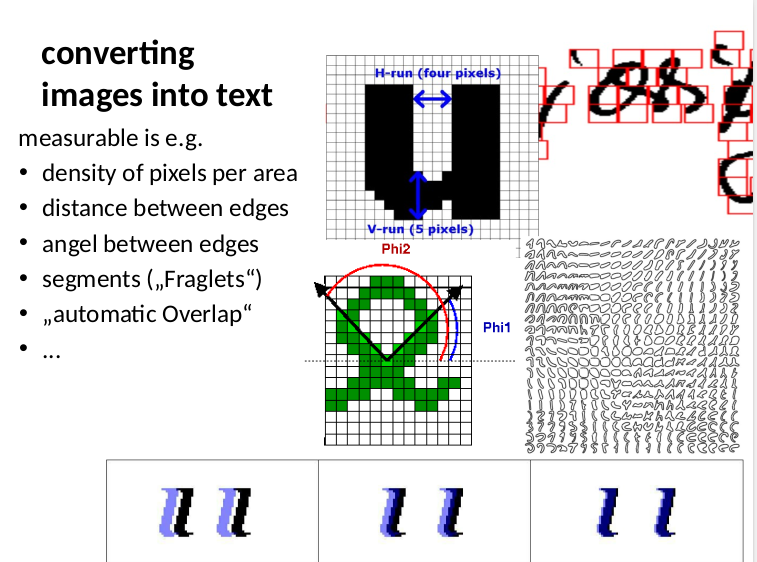
\includegraphics[width=\textwidth]{img/ocr1.png}
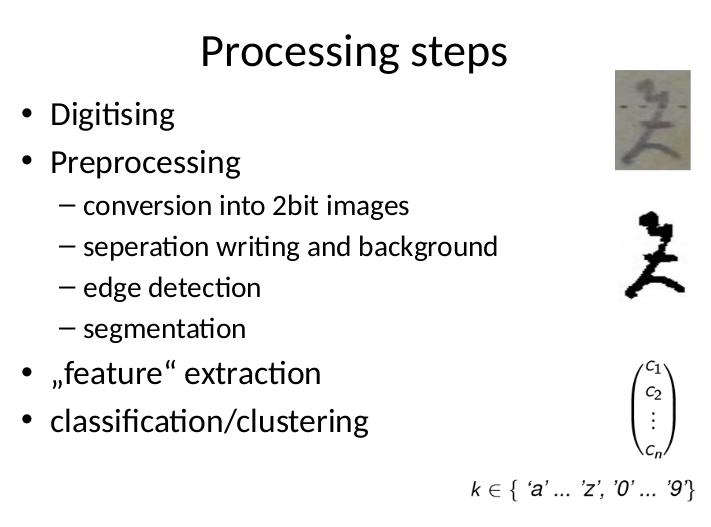
\includegraphics[width=\textwidth]{img/ocr2.png}
\end{columns}

\framebreak 

\begin{columns}
\column{0.48\textwidth}
\begin{block}{Typical phenomena}
\begin{itemize}
\item “Special characters"
\item Abbreviations
\item damaged or unreadable text
\item additions, deletions, substitutions, corrections
\item editorial interventions (emendations and conjectures)
\item  editorial additions or omissions
\end{itemize}
\end{block}

\column{0.48\textwidth}

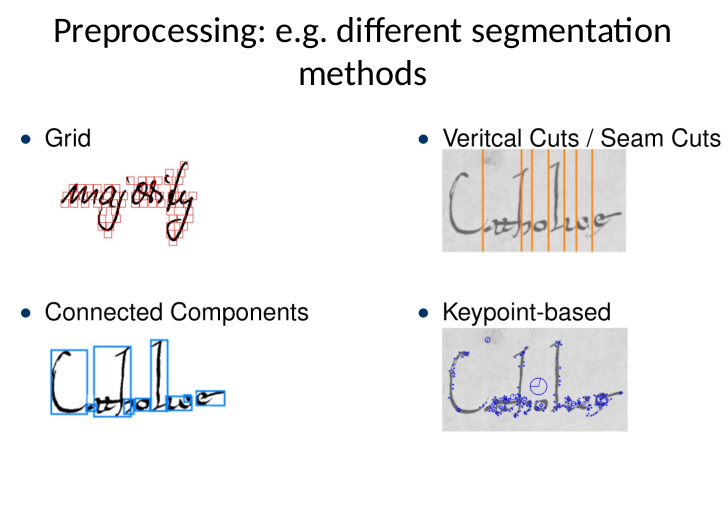
\includegraphics[width=\textwidth]{img/ocr3.png}
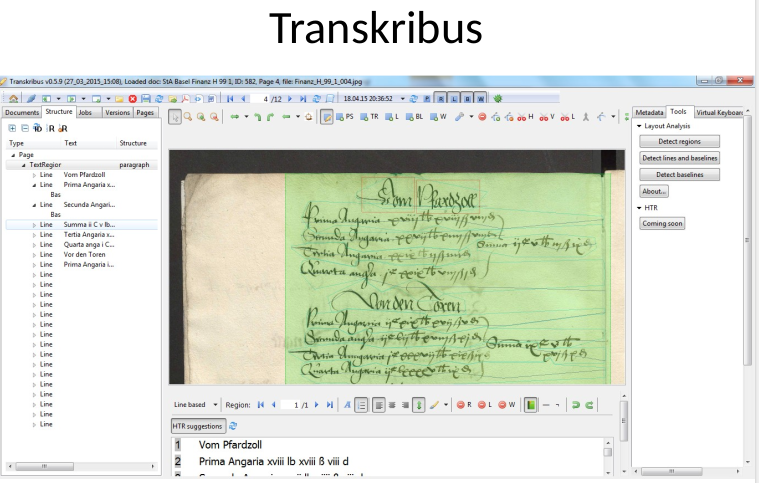
\includegraphics[width=\textwidth]{img/ocr4-transkribus-app.png}

\end{columns}

\end{frame}
%-----------------------------------------------------

\begin{frame}{What is Transkribus?}
    \begin{block}{Transkribus}
       \begin{quote}
           \dots{}is a comprehensive platform for the digitisation, AI-powered text recognition, transcription and searching of historical documents. (\href{https://readcoop.eu/transkribus/}{source})
       \end{quote}
    \end{block}
    \begin{itemize}
        \item we're using the web version TranskribusLite: \protect\url{https://transkribus.eu/lite}
        \begin{itemize}
            \item for more complexity (which you might not need), download the software (Transkribus eXpert)
            \item Lite is easier to learn \& has only the essentials.
            \item you need an account and to buy credits after you have used up your initial 200
            \item print \& manuscript text recognition have different pricing
            \item there are stipends
        \end{itemize}        
    \end{itemize}
\end{frame}


%-----------------------------------------------------
\begin{frame}{Transkribus: Lite versus eXpert}
    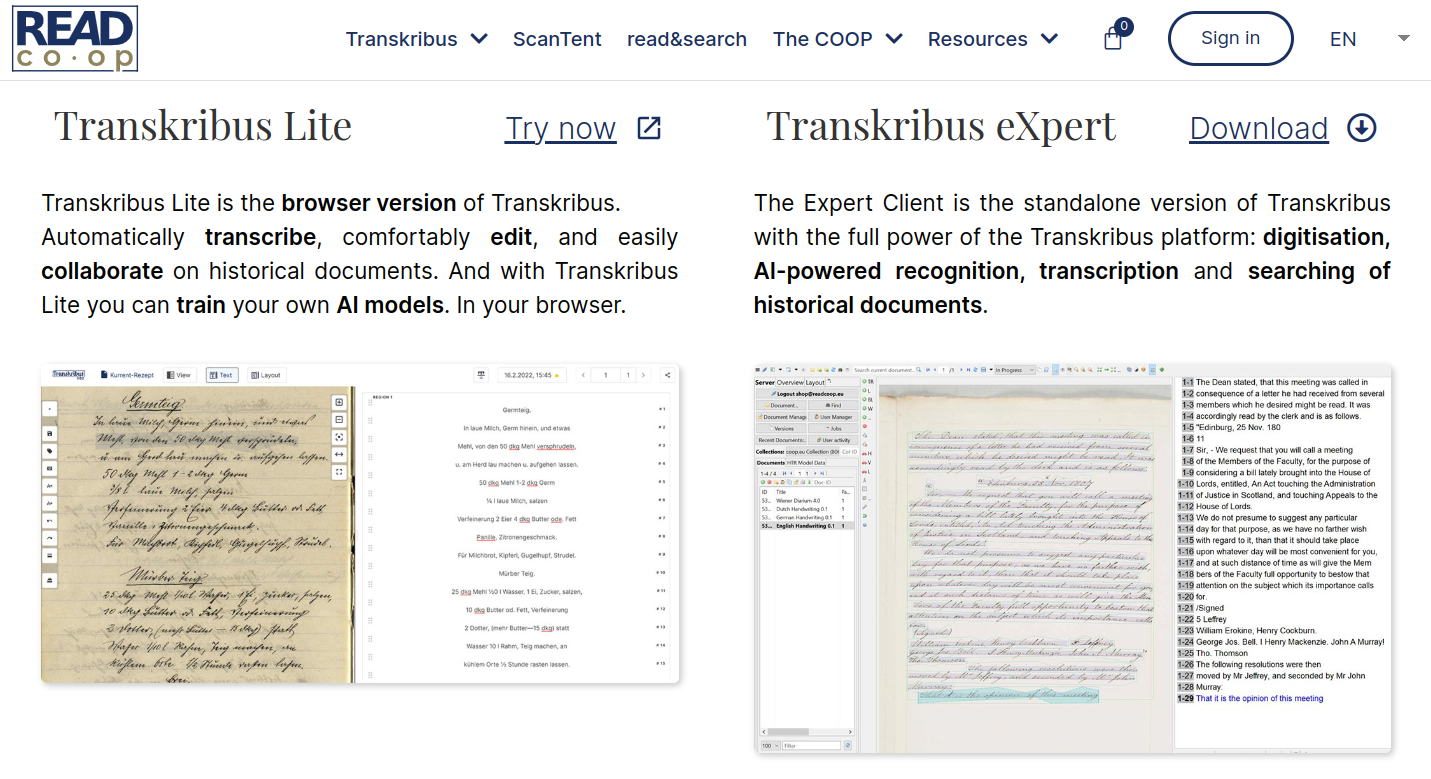
\includegraphics[width=0.95\textwidth]{img/transkribus-versions.png}
\end{frame}
%-----------------------------------------------------
\begin{frame}{Transkribus: How to guides}
    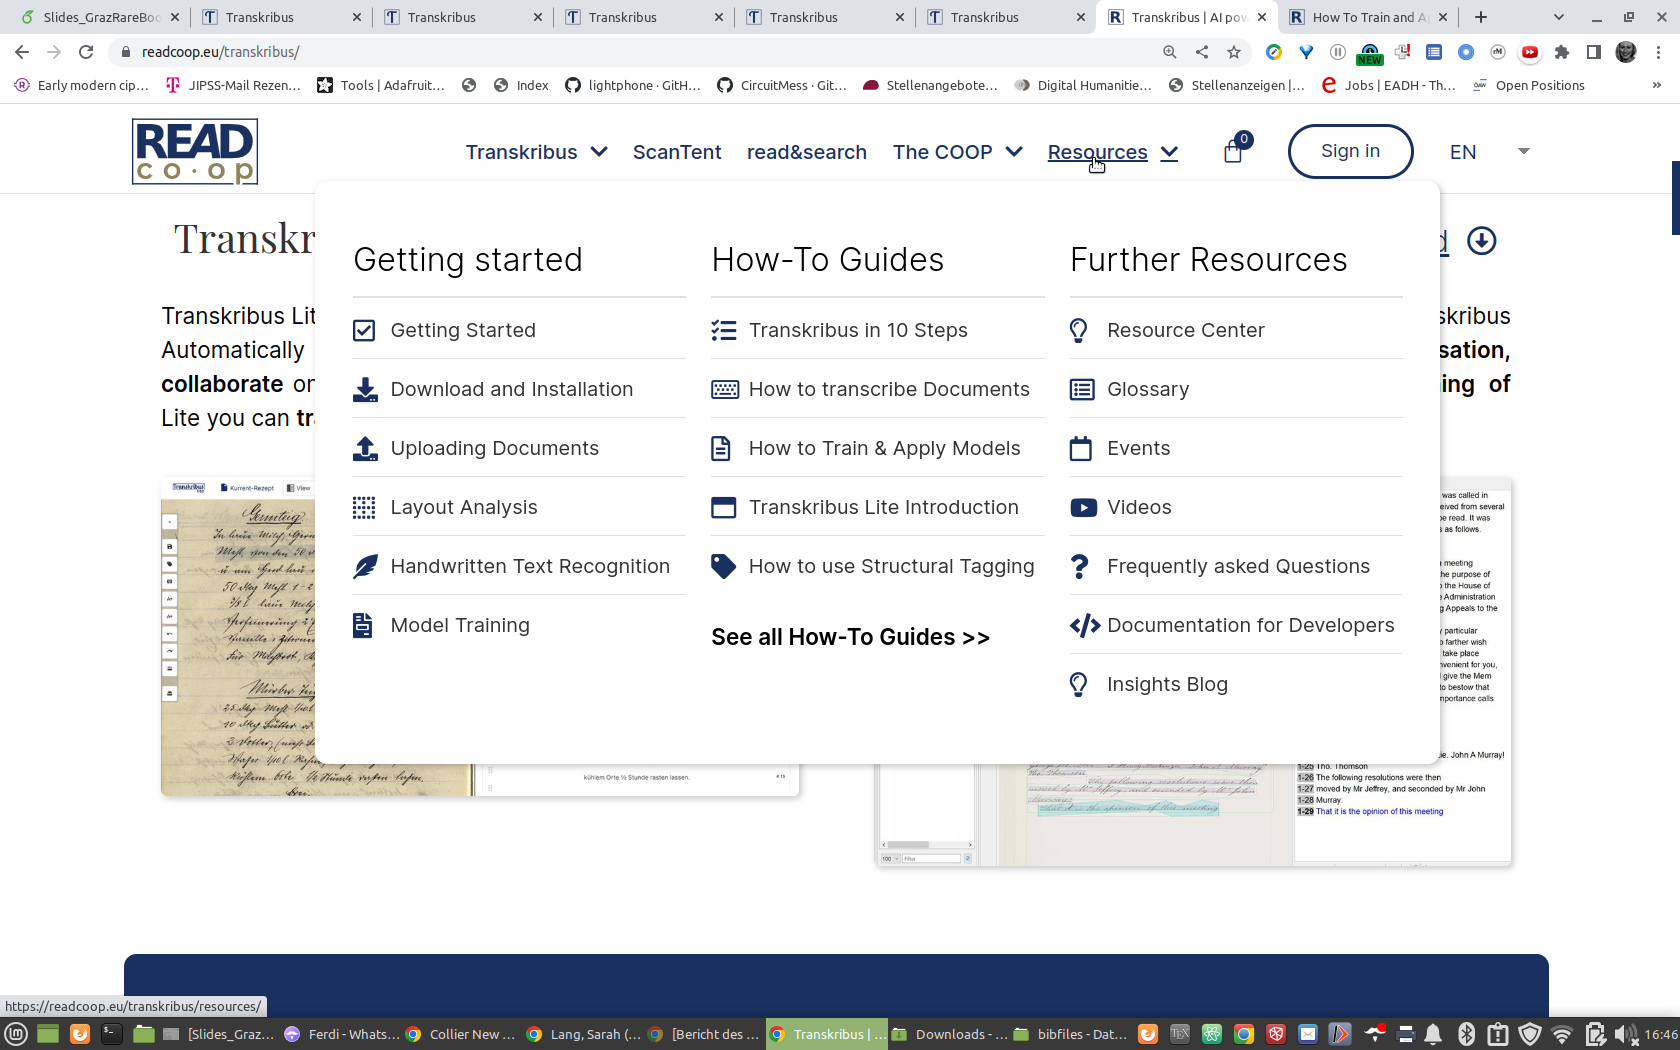
\includegraphics[width=0.95\textwidth]{img/transkribus-resources.png}
\end{frame}
%-----------------------------------------------------
\begin{frame}{Transkribus: Creating transcriptions to train your own model}
    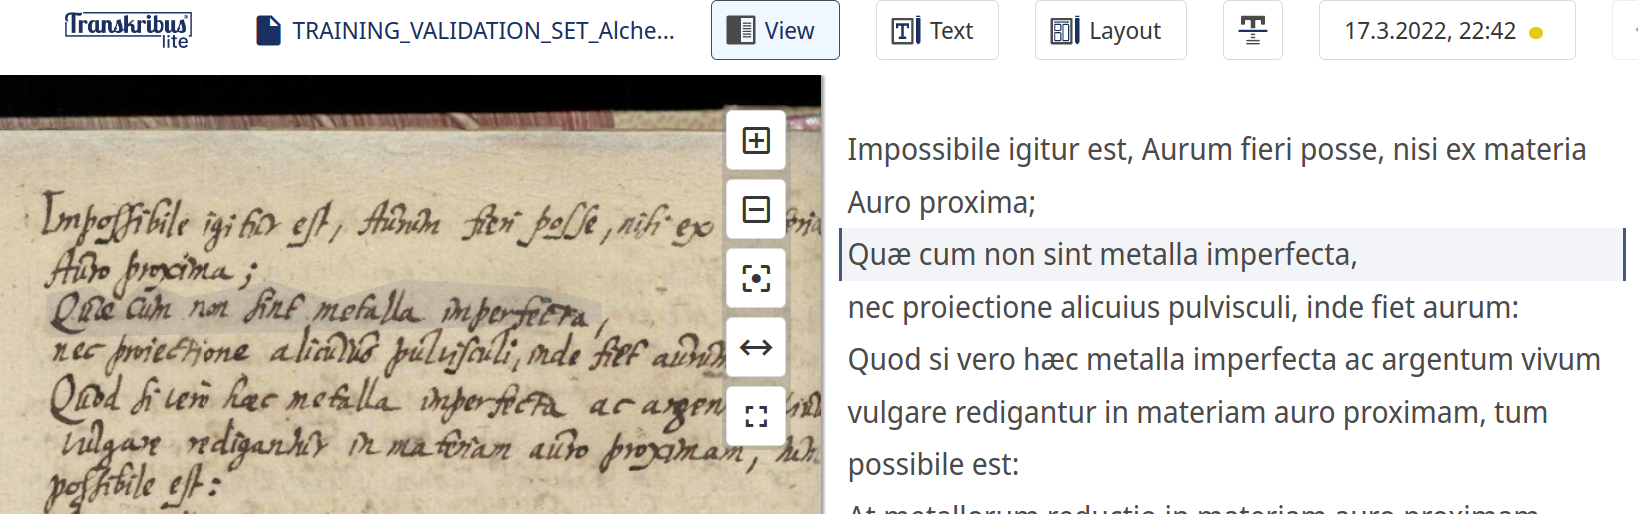
\includegraphics[width=0.95\textwidth]{img/transkribus-training1.png}
    \begin{itemize}\small
        \item first, transcribe a number of pages 
        \begin{itemize}\footnotesize
            \item recommended: 25--75
            \item depending on print or handwritten
            \item you can build on base models (should be similar)
            \item you can speed up the process by creating a model, running it on new pages, correcting them and then repeating the process
            \item correcting is usually still faster than transcribing from scratch
        \end{itemize}
        \item be mindful to adhere to the transcription guidelines you want the model to learn
        \item train your model using the gold-standard transcriptions
        \item use the model on the pages you want transcribed
        \item there will probably be errors: fix them \& use the extra training data created thus to improve the model by retraining it
        \item consider publishing your model if it's of reusable quality
    \end{itemize}
\end{frame}
%-----------------------------------------------------
\begin{frame}{Transkribus: Configuring your model}
    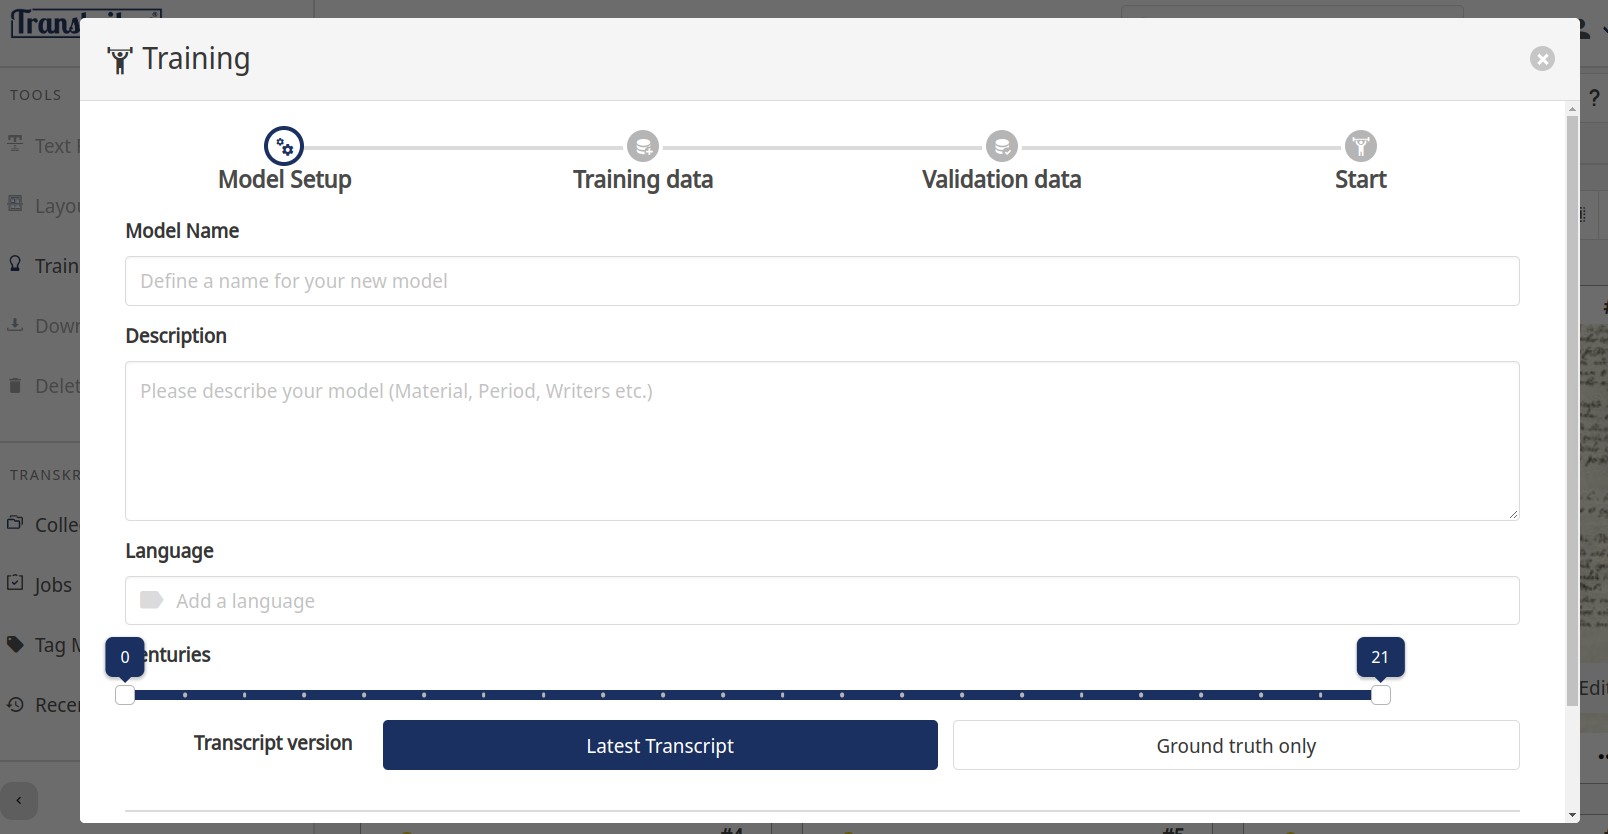
\includegraphics[width=0.95\textwidth]{img/transkribus-training2.png}
\end{frame}


%-----------------------------------------------------
\begin{frame}{Transkribus: further resources}
    \begin{itemize}
        \item \emph{How to historical text recognition: A Transkribus Quickstart Guide}, \LaTeX{}-Ninja Blog, 10. November 2019, \href{https://latex-ninja.com/2019/11/10/how-to-historical-text-recognition-a-transkribus-quickstart-guide/}{URL}. \alert{$\to$ how to reuse exisiting models for print on the example of the Noscemus GM4}
        \item \emph{Training my own Handwritten Text Recognition (HTR) model on Transkribus Lite}, \LaTeX{}-Ninja Blog, 22. March 2022, \href{https://latex-ninja.com/2022/03/22/training-my-own-handwritten-text-recognition-htr-model-on-transkribus-lite/}{URL}. \alert{$\to$ experiences training my own model}
    \end{itemize}
\end{frame}


\section{TEI for Digital Editing}
%-----------------------------------------------------
\begin{frame}[allowframebreaks,fragile]{TEI for Digital Editing}

\subsection{TEI elements relevant to editing}
\metroset{block=fill}\small

\begin{columns}
\column{0.3\textwidth}
TEI can describe the structure of a text, e.g.
\begin{itemize}
\item  speaker, verse line, stage directives
\item  greeting, signature
\item  Visual aspects of the script
\item  special characters, new lines
\end{itemize}

\begin{xmlcode}
<fw place="top-centre" type="head">Poëms.</fw>
<fw place="top-right" type="page-no">29</fw>
\end{xmlcode}

\column{0.68\textwidth}\vspace{-3em}
\begin{block}{Simple layout markup}\footnotesize
\begin{itemize}
\item  beginning of a new \textbf{line}: \texttt{<lb/>}
\item  beginning of a new \textbf{page}: \texttt{<pb/>} \texttt{@n} for an explicit numbering
\item  beginning of a new \textbf{column}: \texttt{<cb/>}
\item  \textbf{highlighted} text: \texttt{<hi>}
\begin{itemize}\scriptsize
    \item Attribute \texttt{@rend} to describe the appearance
    \item Alternative encoding: \emph{<foreign>}, \emph{<emph>}, \emph{<distinct>}
\end{itemize}
\item  graphical elements in the text: \texttt{<figure>}
\item  \texttt{<fw>} (forme work) contains a running head (e.g.
a header, footer), \textbf{catchword}, or similar material
appearing on the current page.
\end{itemize}
\end{block}
\end{columns}


\framebreak

\begin{columns}
\column{0.48\textwidth}
\begin{alertblock}{Documenting particularities of the writing surface}\scriptsize
\begin{description}
\item[<damage>] \texttt{@agent, @degree, @unit, @quantity, @extent, @precision, @scope}
\item[<unclear>]
\item[<gap>] any ommission in the transcription -- @reason, e.g. sampling, inaudible, irrelevant, cancelled
\end{description}
\end{alertblock}


\includegraphics[width=0.5\textwidth]{img/tei-unclear.png}
\vspace{2em}

\begin{xmlcode}
<gap reason=“wormhole" quantity="5" unit="character"/>
<damage agent=“coffee” quantity=“3” unit=“line”/>
\end{xmlcode}

\column{0.5\textwidth}
\begin{alertblock}{Other important attributes}
\begin{description}\scriptsize
    \item[@cert(ainty)] how certain you are about the suggested transcription?
    \item[@resp(onsibility)] who did it?
    \item[@evidence] where you got the clues from (internal, external, conjecture)?
\end{description}
\end{alertblock}

\begin{xmlcode}
I <subst>
 <add place="above">might</add>
  <del>
   <unclear reason="overinking"
      cert="medium" resp="#LDB"> 
      should</unclear>
  </del> </subst> have
\end{xmlcode}
\end{columns}


\end{frame}

%-----------------------------------------------------
\begin{frame}[allowframebreaks,fragile]{Transcription}
\subsubsection{Transcription}
\metroset{block=fill}

\begin{columns}
\column{0.48\textwidth}
\begin{itemize}\small
\item  OCR (Optical Character Recognition) -- e.g. Transkribus (transcription support)
\item  also:  Transkribus Keyword Spotting 
\item  also:  fuzzy search which should also find the word if it's mistranscribed
\item  Writer identification
\end{itemize}

\column{0.48\textwidth}

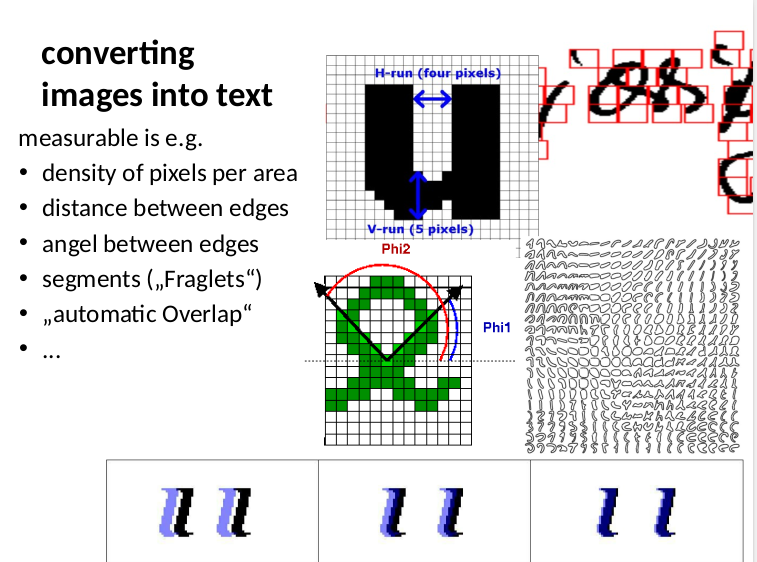
\includegraphics[width=\textwidth]{img/ocr1.png}
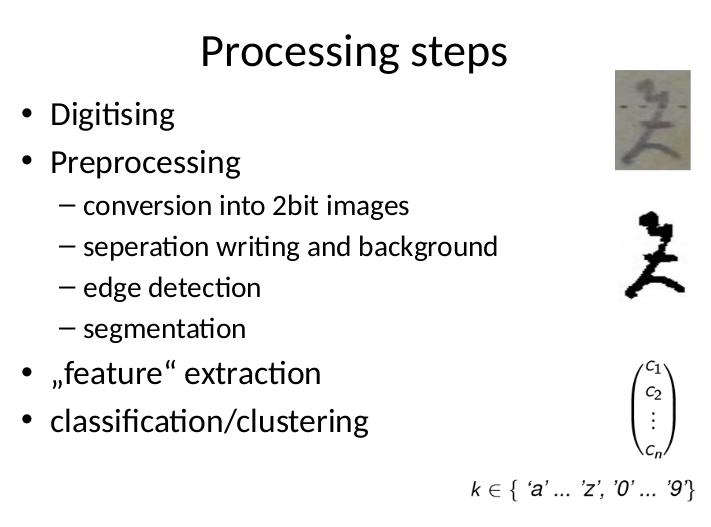
\includegraphics[width=\textwidth]{img/ocr2.png}
\end{columns}

\framebreak 

\begin{columns}
\column{0.48\textwidth}
\begin{block}{Typical phenomena}
\begin{itemize}
\item “Special characters"
\item Abbreviations
\item damaged or unreadable text
\item additions, deletions, substitutions, corrections
\item editorial interventions (emendations and conjectures)
\item  editorial additions or omissions
\end{itemize}
\end{block}

\column{0.48\textwidth}

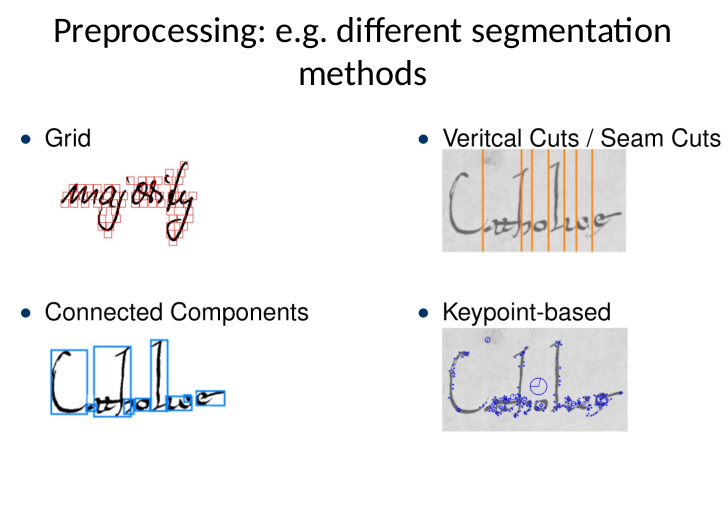
\includegraphics[width=\textwidth]{img/ocr3.png}
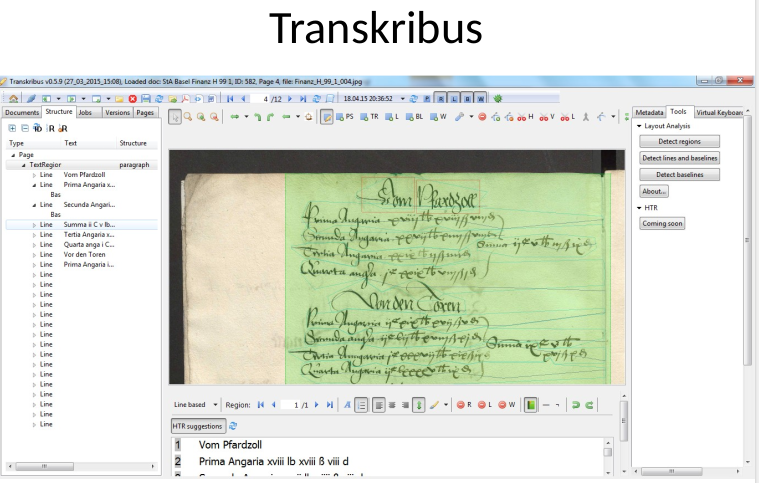
\includegraphics[width=\textwidth]{img/ocr4-transkribus-app.png}

\end{columns}

\framebreak

Transcriptions contain: 
\begin{columns}
\column{0.4\textwidth}
\begin{itemize}
\item  layout
\item  additions
\item  corrections
\item  modifications
\item  voids, space, holes, gaps \dots
\item  alternative transcriptions
\item  editorial interventions
\item  Enhanced transcription
\end{itemize}

\column{0.55\textwidth}
\begin{xmlcode}
<pb>, <lb>, <cb>, <hi>, <g>, 
<handShift/>
<add>, <addSpan>,
<corr>, <del>, <delSpan>, <sic>
<subst>
<gap>, <damage>
<choice>, <alt>
<unclear>, <supplied>, <reg>
<add>, <addSpan>, <corr>, <choice>, 
<damage>, <del>, <delSpan>, 
<restore>, <gap>, <sic>
\end{xmlcode}
\end{columns}

\end{frame}


%-----------------------------------------------------
\begin{frame}[fragile]{Genetic Edition}
\metroset{block=fill}

\begin{columns}
\column{0.48\textwidth}
\begin{block}{Critique Génétique}\footnotesize
\textbf{Research interest:} Reconstruct the writing process in the working manuscripts of the author
\end{block}

\column{0.48\textwidth}
\begin{xmlcode}
That's <del xml:id="del1">
superfluous 
<restore>
 <redo target="del2" /> 
 <del xml:id="del2">deleted</del> 
</restore> </del>
text.
\end{xmlcode}
\end{columns}



\begin{columns}
\column{0.48\textwidth}
\begin{xmlcode}
<zone>
 <line>Alone
  <seg type="alternative" 
   xml:id="alt1"> before </seg>
  <add place="above" 
       type="alternative"
       xml:id="alt2">beside</add> 
  his native river—
 </line>
 <alt targets="#alt1 #alt2" 
      mode="excl" weights="01"/>
</zone>
\end{xmlcode}
\column{0.48\textwidth}
\begin{xmlcode}
He sat <seg type="transposition" 
xml:id="trans1"> at
his table</seg> 
<seg type="transposition"
xml:id="trans2"> head on hands
</seg>.

<listTranspose>
<transpose>
  <ptr target="#trans2"/>
  <ptr target="#trans1"/>
</transpose>
</listTranspose>
\end{xmlcode}
\end{columns}

\end{frame}


%-----------------------------------------------------
\begin{frame}[fragile]{The script: palaeography}
\metroset{block=fill}

\begin{columns}
\column{0.58\textwidth}
\begin{itemize}
\item  soft hyphen: \texttt{@break=“no”}
\item  \texttt{@rend | @rendition}
\begin{itemize}
    \item \texttt{@rend}: verbal description; each word describes a single facet (\texttt{rend=“indented:5cm”})
    \item \texttt{@rendition}: reference to description of the rendition in the \texttt{teiHeader//encodingProfile}
\end{itemize}
\item  „special characters":
\begin{itemize}
    \item \texttt{<g>}
    \item Does it exist in Unicode? (\protect\url{http://www.unicode.org}). As an entity in XML:
\begin{xmlcode}
&#x[hexadecimal code];
&#[decimal code];
\end{xmlcode}
\item Search \protect\url{https://unicode-table.com/}
\end{itemize}
\end{itemize}

\column{0.38\textwidth}
\begin{block}{Unicode for historical texts}\scriptsize
\begin{itemize}
\item  \emph{Combining Diacritical Marks} (0300–036F) and \emph{Supplement} (1DC0–1DFF): Superscripts, Subscripts
\item  \emph{Latin Extended Additional} (1E00–1EFF): characters with diacritics
\item  \emph{Latin Extended-D} (A720–A7FF): Ligatures, abbreviations, \dots
\item  \emph{General Punctuation} (2000–206F) and \emph{Supplement} (2E00–2E7F)%: \#\#Hochpunkte etc.
\item  \emph{Ancient Symbols} (10190–101CF): roman measurements, coins\dots
\item Search unicode entities: \protect\url{https://unicode-table.com/}
\end{itemize}
\end{block}
\end{columns}


\end{frame}
%-----------------------------------------------------
\begin{frame}[fragile]{Editorial interventions}
\metroset{block=fill}

\begin{columns}
\column{0.48\textwidth}
\begin{itemize}
    \item expansion of abbreviations
    \item Conjectures
    \item Normalisations
\end{itemize}
\column{0.48\textwidth}
\begin{itemize}
\item \texttt{<abbr>, <expan>} plus \texttt{<am>, <ex>}
\item \texttt{<sic>, <corr>}
\item \texttt{<orig>, <reg>}
\end{itemize}
\end{columns}\bigskip

\begin{block}{All these can be paired:}
\begin{itemize}
    \item General for all editorial interventions: \texttt{<choice>}.
    \item Explicitly for substitutions: \texttt{<subst>}.
    \item \texttt{<supplied>} for additions by the editor
    \item \texttt{<unclear>} for unreadable text (\texttt{@reason, @agent, @hand})
\end{itemize}
\end{block}

\end{frame}
%-----------------------------------------------------
\begin{frame}[allowframebreaks,fragile]{Abbreviations}
\metroset{block=fill}\small 

\begin{columns}
\column{0.42\textwidth}
In Western MS, we usually distinguish:
\begin{itemize}\scriptsize
\item  \textbf{Suspensions:} the first letter or letters of the word are written, generally followed by a point : for example ‘e.g.’ for ‘exempla gratia’
\item  \textbf{Contractions:} both first and last letters are written, generally with some mark of abbreviation such as superscript strokes, or points : e.g. ‘Mr.’ for ‘Mister’
\item  \textbf{Brevigraphs:} Special signs such as the Tironian nota used for ‘et’, the letter p with a barred tail used for ‘per’, the letter c with a circumflex used for ‘cum’/’con’ etc.
\item  \textbf{Superscripts:} Superscript letters (vowels or consonants) used to indicate various kinds of contraction: e.g. ‘w’ followed by superscript ‘ch’ for ‘which’.
\end{itemize}

\column{0.56\textwidth}
\begin{itemize}\small 
\item  \texttt{<expan>} The element content is considered as the expansion of an abbreviation. In the text: USA $\to$ transcription: 
\begin{xmlcode}
<expan>United States of America</expan>
\end{xmlcode}
\item  \texttt{<abbr>} The element content is an abbreviation
\begin{xmlcode}
<abbr>USA</abbr>
\end{xmlcode}
\item  \texttt{<ex>} (expansion) and \texttt{<am>} (abbreviation mark) for the  omitted part of the abbreviation, e.g.
\begin{xmlcode}
e<ex>xempla</ex> g<ex>ratia</ex>
e<am>.</am> g<am>.</am>
\end{xmlcode}
\end{itemize}
\end{columns}

\framebreak

Abbreviations can also be considered as alternatives: \texttt{<choice>}, e.g. `Zum Beispiel' and `z.B.':
\begin{xmlcode}
<choice>
 <expan>Zum Beispiel</expan>
 <abbr>Z.B.</abbr>
</choice>
\end{xmlcode}

Or respectively:
 \begin{xmlcode}
Z<choice>
   <am>.</am>
   <ex>um</ex>
  </choice>
  
B<choice>
   <am>.</am>
   <ex>eispiel</ex>
 </choice>
\end{xmlcode}


\end{frame}

%----------------------------

\begin{frame}{Transcription = Interpretation}
\metroset{block=fill}\small

\begin{columns}
\column{0.48\textwidth}\small
`gemination dash' – possible solutions:
\begin{itemize}\footnotesize
\item  Uncommented expansion
\item  Unicode m with "combining macron"
\item  Encoding as an XML-Entity
\item  \texttt{<g>} refering to \texttt{<charDecl>}
\item  Only \texttt{<am/>} for the stroke
\item  Only \texttt{<ex>} for the expansion
\item  As a \texttt{<choice>} with \texttt{<abbr>} and \texttt{<expan>}, the first incl.
a abbreviation mark \texttt{<am>} and the second the
expansion \texttt{<ex>}
\end{itemize}

\begin{block}{Gemination dash}\scriptsize
horizontal, bended or curved stroke above a nasal letter indicating the omission of a further instance of the same letter.~(\href{https://www.degruyter.com/database/WSK/entry/wsk_id_wsk_artikel_artikel_14933/html?lang=en}{source})
\end{block}

\column{0.48\textwidth}
\begin{block}{Modifications}\footnotesize
\begin{itemize}
\item  addition, deletion, substitution, transpose, \emph{or:}
\item  modification (represents any kind of general
modification without interpretation)
\end{itemize}
\end{block}

\begin{alertblock}{Changing writer}\footnotesize
\begin{description}
\item[<handShift />] \texttt{@new} : the hand which writes from this place onward
\item[<handDesc>] (part of \texttt{msDesc}) 
\item[<handNotes>] (part of \texttt{profileDesc})
\item[<handNote>] for a particular description
\item[@xml:id] an identifier for the hand
\end{description}
\end{alertblock}
\end{columns}


\end{frame}

%-----------------------------------------------------
\begin{frame}[allowframebreaks,fragile]{Text and images}
\subsubsection{Text and images}

\metroset{block=fill}
\begin{columns}
\column{0.4\textwidth}
Images of a text are encoded in a \texttt{facsimile} --
structure parallel to \texttt{teiHeader} and \texttt{text}:
\begin{xmlcode}
<tei>
  <teiHeader>...</teiHeader>
  <facsimile> ...</facsimile>
  <text>...</text>
</tei>
\end{xmlcode}

\column{0.58\textwidth}
\begin{alertblock}{\texttt{<facsimile>}}\footnotesize
\begin{itemize}
\item  \texttt{<surface>} = something meant to be seen
\begin{itemize}
    \item \texttt{@uly, @ulx; @lrx, @lry} =upper left x/y- and lower right y/x coordinates
    \item  coordinates form a grid, which can be referred $\to$ \texttt{@ulx} and \texttt{@uly} are usually 0
\end{itemize}
    \item \texttt{<graphic>}: image, \texttt{@url} : image file
     \item  \texttt{<zone>} = an area on the surface. Coordinates refer to the grid defined in \texttt{@uly}, \texttt{@ulx}; \texttt{@lrx, @lry} of the \texttt{<surface>}.
\end{itemize}
\end{alertblock}
\end{columns}


\framebreak

\begin{columns}
\column{0.48\textwidth}
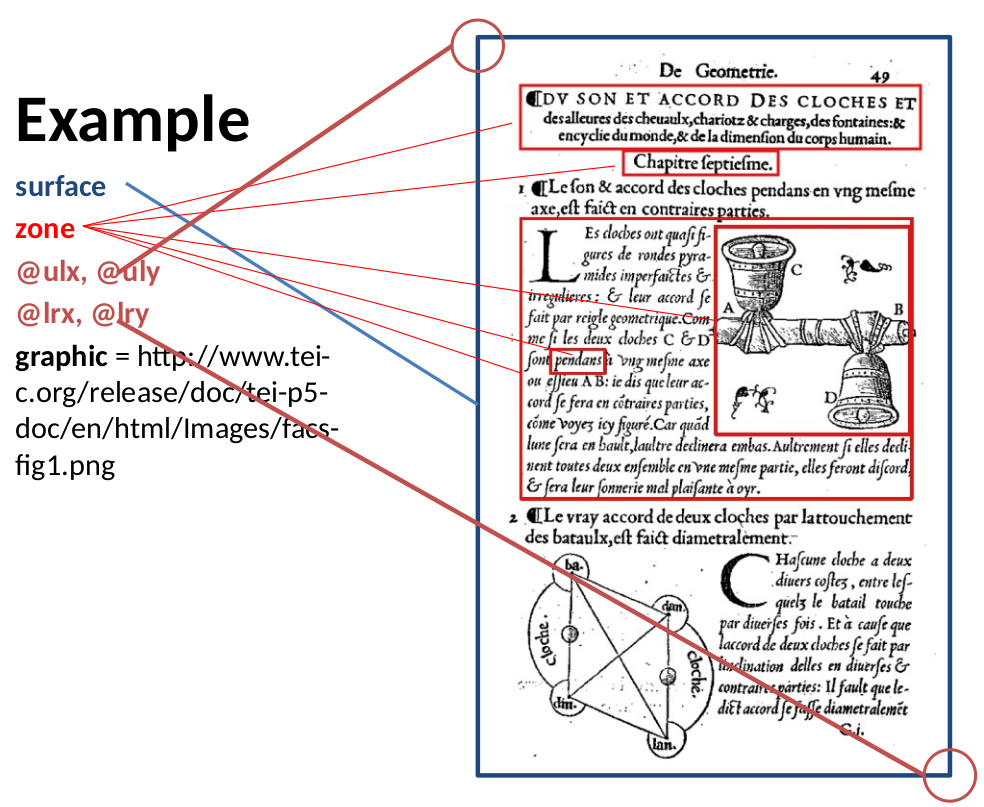
\includegraphics[width=\textwidth]{img/facs1.png}
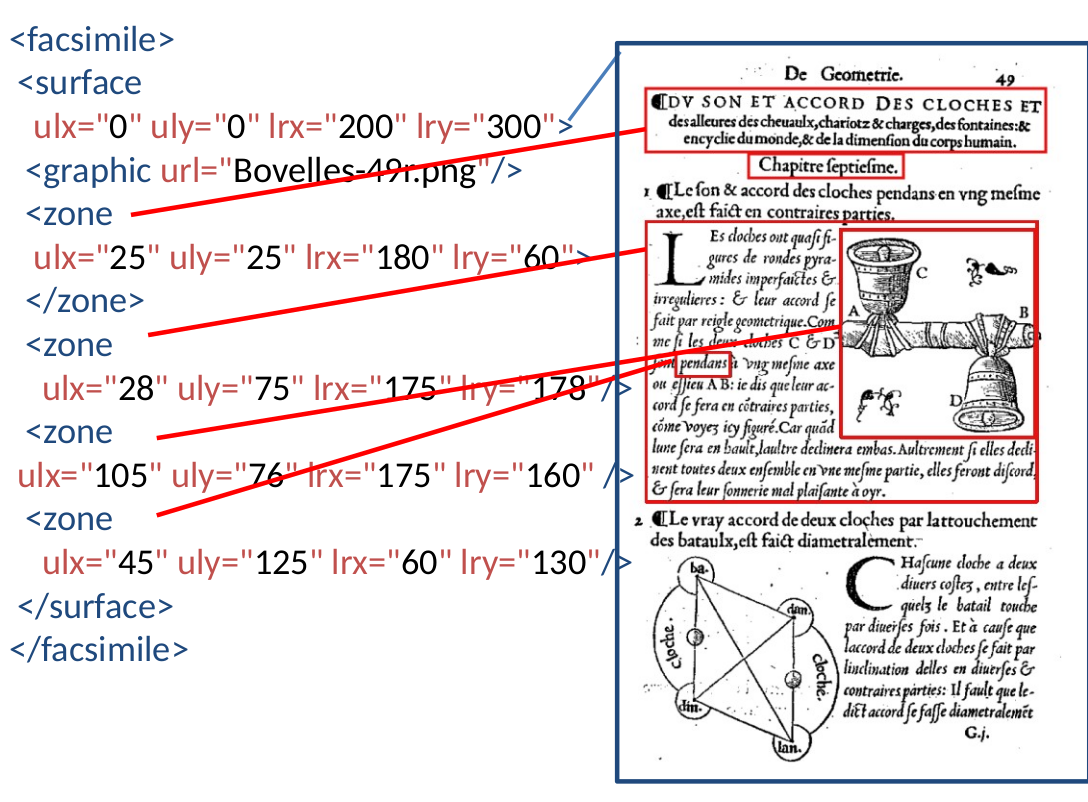
\includegraphics[width=\textwidth]{img/facs2.png}
\column{0.48\textwidth}
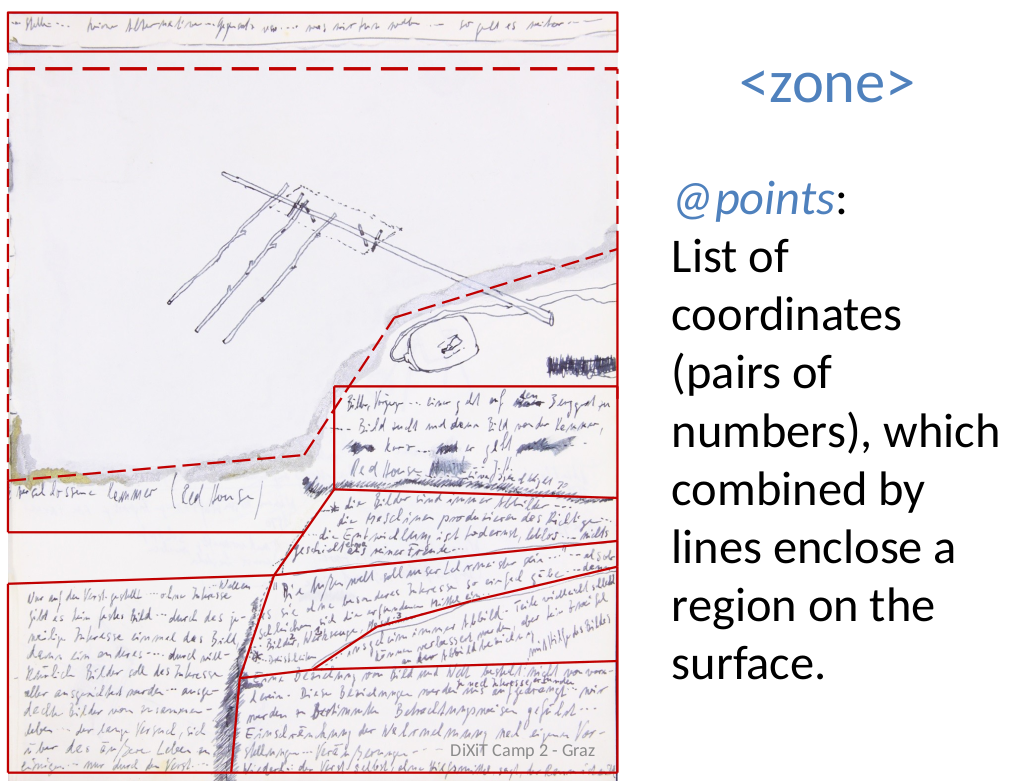
\includegraphics[width=\textwidth]{img/facs3.png}
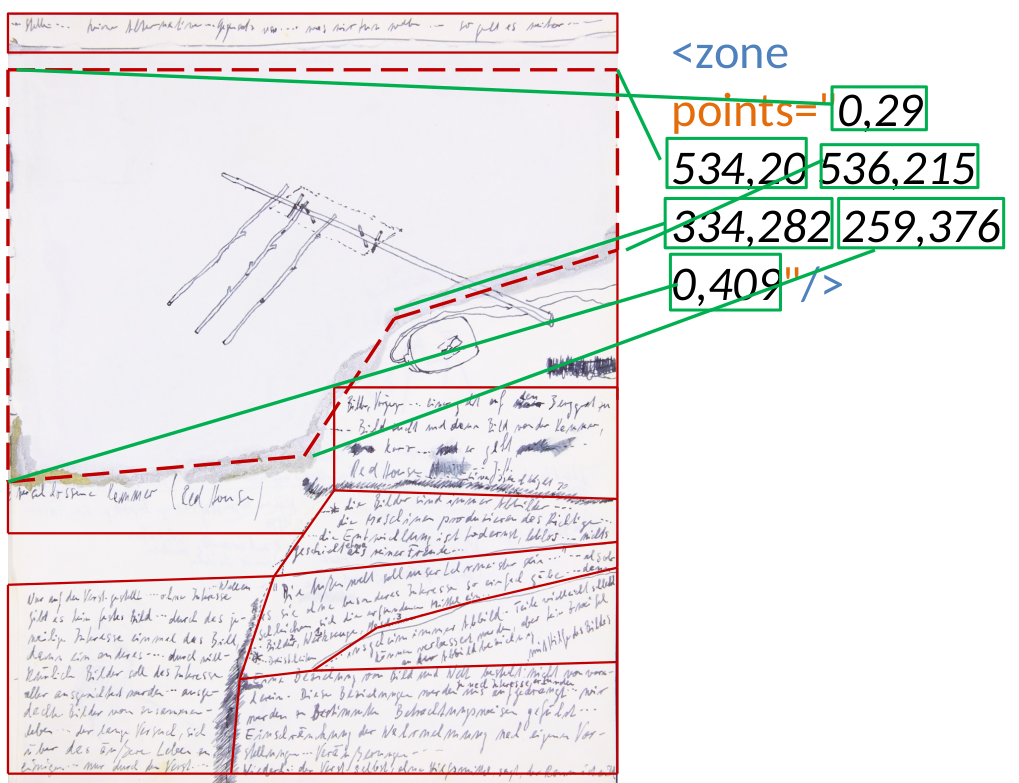
\includegraphics[width=\textwidth]{img/facs4.png}
\end{columns}

\framebreak

\begin{columns}
\column{0.48\textwidth}

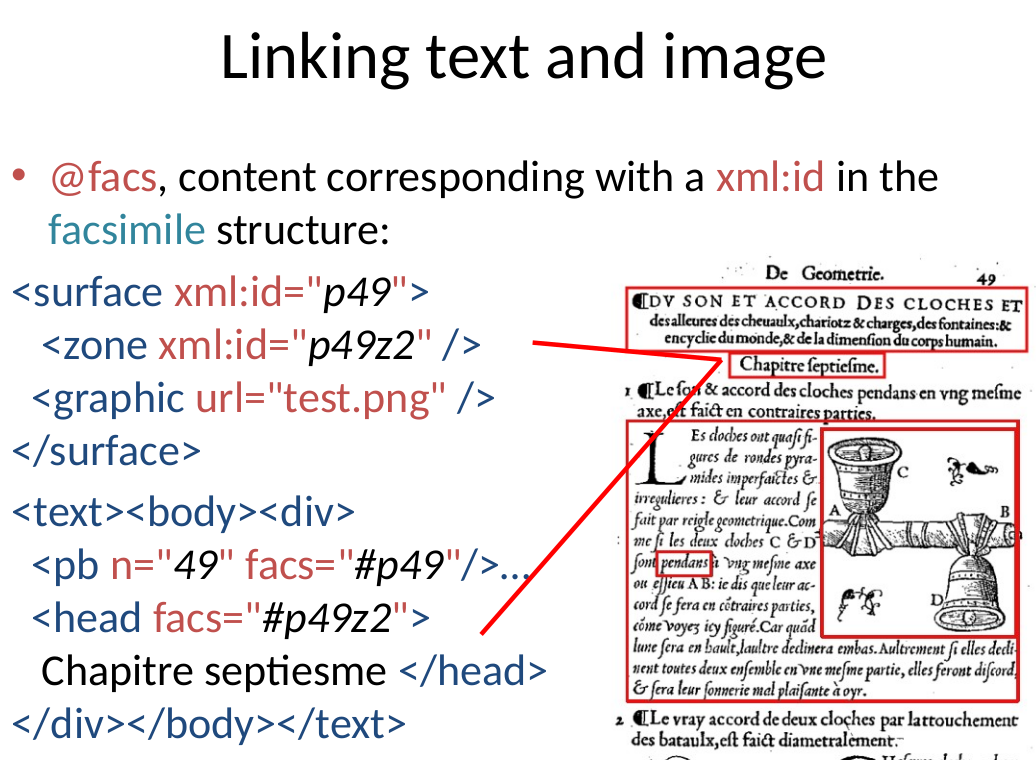
\includegraphics[width=\textwidth]{img/facs5.png}
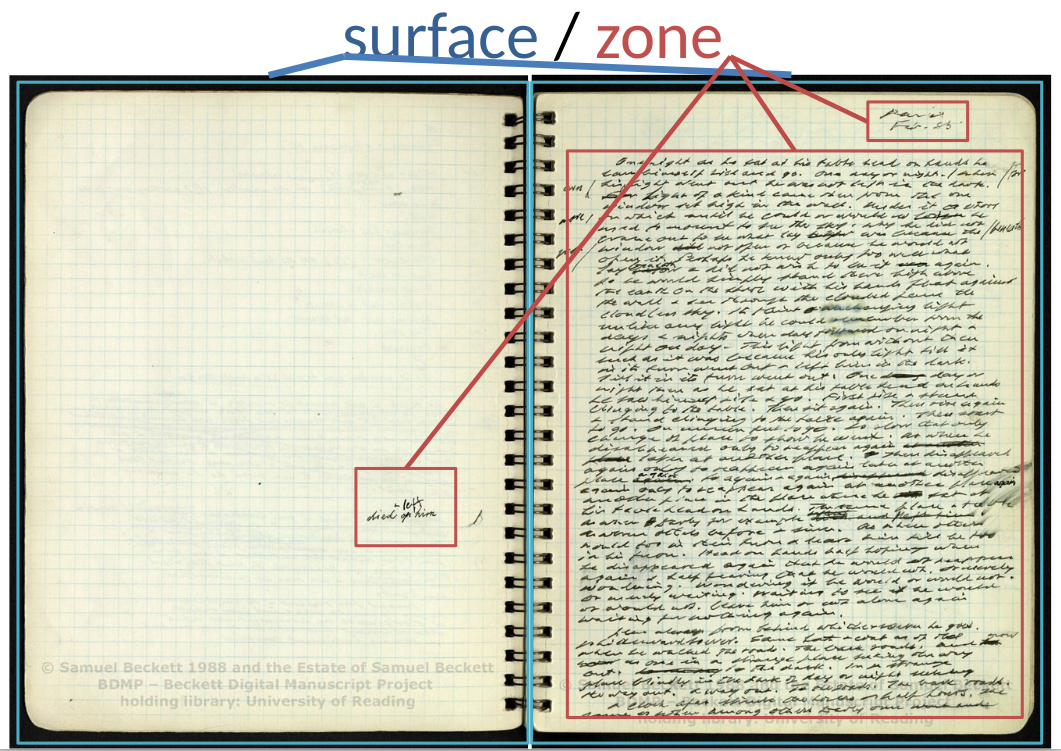
\includegraphics[width=\textwidth]{img/facs6.png}

\column{0.48\textwidth}
\begin{block}{Tools for text-image linking}
\begin{enumerate}\footnotesize
\item  \textbf{Image markup tool} (Martin Holmes, \protect\url{http://www.tapor.uvic.ca/~mholmes/image_markup/index.php})
\item  \textbf{TextGridLab:} http://www.textgridlab.de
\item  \textbf{T-PEN} (\protect\url{http://www.t-pen.org})
%\item  Faust-Edition: \protect\url{https://github.com/faustedition/ext-imageannotation}
\item \protect\url{http://imagecoordinates.com}
\end{enumerate}
\end{block}
\end{columns}

\framebreak


\begin{columns}
\column{0.48\textwidth}
\begin{block}{Embedded transcription}
\begin{itemize}\footnotesize
\item  "Embedded transcription": Text directly in \texttt{<surface>}
\item  \texttt{Relevant elements:} \texttt{<sourceDoc>}, \texttt{<surface>}, \texttt{<zone>}, \texttt{<line>}, \texttt{@rotate}
\end{itemize}
\end{block}

\column{0.48\textwidth}
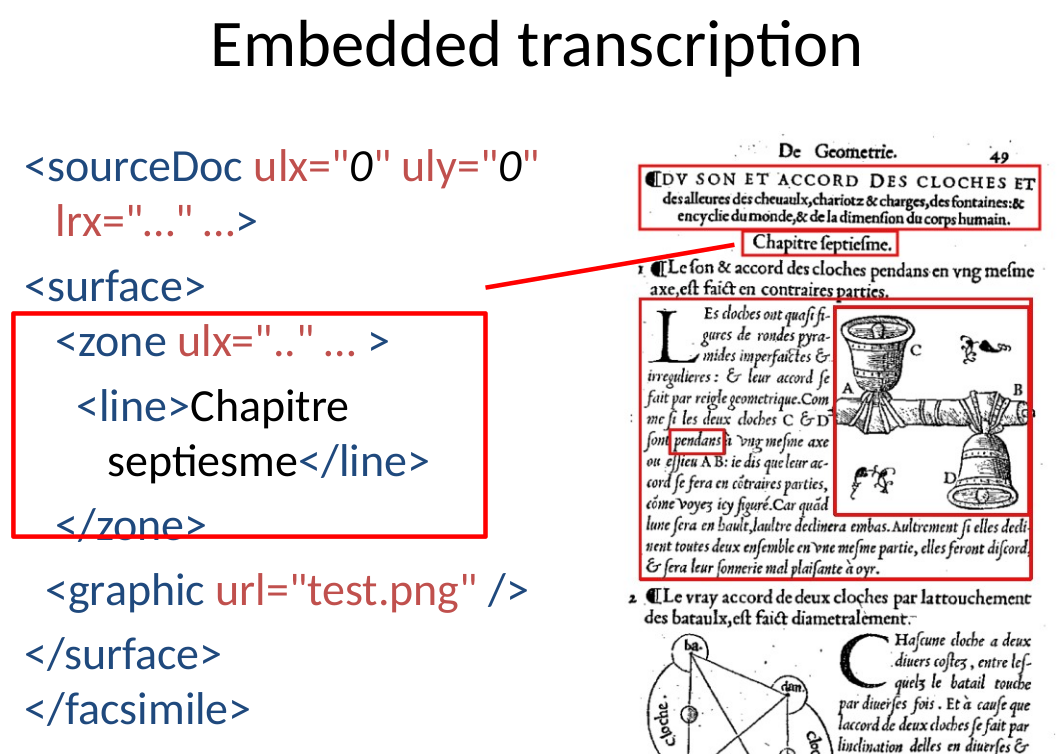
\includegraphics[width=\textwidth]{img/facs-embedded.png}
\end{columns}

\begin{xmlcode}
<sourceDoc>
 <surfaceGrp n="leaf1">
  <surface facs="page1.png"> <zone>All the writing on page 1</zone> </surface>
  <surface>
   <graphic url="page2-highRes.png"/>
   <zone> <line>A line of writing on page 2</line> </zone>
  </surface>
 </surfaceGrp>
</sourceDoc>
\end{xmlcode}

\end{frame}


%-----------------------------------------------------
\begin{frame}[allowframebreaks,fragile]{Critical Apparatus}
\subsubsection{Critical Apparatus in TEI}
\metroset{block=fill}
\dots aims at documenting the variants of a text in the witnesses of textual transmission.\medskip 

\begin{columns}
\column{0.48\textwidth}\small
A critical apparatus is encoded with:
\texttt{<app>}, \texttt{<rdg>} / \texttt{<rdgGrp>} and \texttt{<lem>}.
\texttt{<lem>} can contain text not documented in any textual witness.

\begin{xmlcode}
<app>
  <rdg wit="#Sh1">Then</rdg>
  <lem wit="#Sh2">Than</rdg>
</app> is my deede to my most  
<app>
  <lem wit="#Sh1">painted</rdg>
  <rdg wit="#Sh2">pained</rdg>
</app>word:

<app>
    <lem>deed</lem>
    <rdg wit="#Sh1 #Sh2">deede</rdg>
</app>
\end{xmlcode}

\column{0.48\textwidth}
\begin{xmlcode}
<app>
  <lem wit="#Sh2">Than</rdg>
  <rdg wit="#Sh1">Then</rdg>
</app> is my deede to my most  
<app>
  <lem wit="#Sh1">painted</rdg>
  <rdg wit="#Sh2">pained</rdg>
</app>word:

<app>
  <rdg wit="#Sh1">Then</rdg>
  <rdg wit="#Sh2">Than</rdg>
</app> is my deede to my most  
<app>
  <rdg wit="#Sh1">painted</rdg>
  <rdg wit="#Sh2">pained</rdg>
</app>word:
\end{xmlcode}

\end{columns}

\framebreak



\begin{columns}
\column{0.48\textwidth}\small 

The apparatus can be located anywhere as a \texttt{<listApp>}:
\begin{itemize}\footnotesize
    \item in the \texttt{<body>} of the document 
    \item in the \texttt{<back>} in other documents
    \item is referenced by \texttt{@loc}
\end{itemize}

$\to$ \texttt{<rdgGrp>} aggregates several readings of a common type.

\begin{block}{Witness list}
\texttt{@wit} refers to descriptions in the header: 
\texttt{<listWit>} = list of \texttt{<witness>}-elements identified by \texttt{@xml:id} each describing a textual witness e.g. by \texttt{<bibl>}- or \texttt{<msDesc>} elements in \texttt{teiHeader}/\texttt{sourceDesc}
\end{block}

\column{0.48\textwidth}
\begin{xmlcode}
<app>
    <rdgGrp type="orthographic">
        <rdg wit="#Sh1">giue</rdg>
        <rdg wit="#Sh2">give</rdg>
    </rdgGrp>
    <rdg wit="#AS1">have</rdg>
</app>

<listWit>
    <witness xml:id="Sh1">
  <bibl>Folger STC 22276</bibl>
    </witness>
    <witness xml:id="Sh2">
  <bibl>Huntington 69304</bibl>
    </witness>
</listWit>
\end{xmlcode}

\end{columns}

\framebreak


There are different options:
\begin{columns}
\column{0.48\textwidth}
\begin{block}{Location referenced + external}
\begin{xmlcode}
<p><pb n="f13"/><lb n="f13-z1" /> 
Dis ouentúrlich buoch bewiset wye 
von einer Frowen ge<lb/>nannt 
Melusina ...</p>
<!-- ... -->
<listApp><app loc="f13-z1">
    <lem wit="#BR1">ouentúrlich</lem>
    <rdg wit="#SK1">ouentuorlich</rdg>
    <rdg wit="#AS1">abenteürlich</rdg>
</app></listApp>
\end{xmlcode}
\end{block}



\column{0.48\textwidth}
\begin{block}{Double endpoint + external}\footnotesize

The apparatus is integrated into the \texttt{<body>} linked to identifiers for its beginning and its end (e.g. with \texttt{<anchor>}) but encoded anywhere (e.g. in the place where it was located in the printed source); referenced by \texttt{@from} \& \texttt{@to}.

\begin{xmlcode}
<p>Dis <anchor xml:id="A1"/>
ouentúrlich<anchor xml:id="A2"/> buoch
    bewiset wye von einer 
    Frowen ge<lb/>nannt Melusina 
    ...</p>
<!-- ... -->
<app from="#A1" to="#A2">
    <rdg wit="#SK1">ouentuorlich</rdg>
    <rdg wit="#AS1">abenteürlich</rdg>
</app>
\end{xmlcode}
\end{block}

\end{columns}

\framebreak

\begin{columns}
\column{0.48\textwidth}
\begin{block}{Location referenced + inline}
\begin{xmlcode}
<p n="p1">
    Dis ouentúrlich
    <app loc="p1">
        <rdg wit="#SK1">
           ouentuorlich</rdg>
        <rdg wit="#AS1">
           abenteürlich</rdg>
    </app>
    buoch bewiset wye 
    von einer Frowen 
    ge<lb/>nannt Melusina ...
</p>
\end{xmlcode}
\end{block}

\column{0.48\textwidth}

\begin{block}{Double endpoint + internal}\footnotesize
The apparatus is integrated into the \texttt{<body>} after the referenced passage and linked an identifiers for its beginning; referenced by \texttt{@from}.

\begin{xmlcode}
<p n="1">
    Dis <anchor xml:id="a"/>
    ouentúrlich<app from="#a">
        <rdg wit="#SK1">
           ouentuorlich</rdg>
        <rdg wit="#AS1">
           abenteürlich</rdg>
    </app>
    buoch bewiset wye von einer 
    Frowen ge<lb/>nannt Melusina
    ...
</p>
\end{xmlcode}
\end{block}
\end{columns}

\framebreak


\begin{columns}
\column{0.48\textwidth}
Last but not least\dots
\begin{block}{Parallel segmentation}\footnotesize
Encoding the „base text“ as the \texttt{lem} in the \texttt{app}-element. Can be done only inline. Possibility to nest variants.

\begin{xmlcode}
<p n="1">Dis
    <app>
        <lem wit="#BR1">
           ouentúrlich</lem>
        <rdg wit="#SK1">
           ouentuorlich</rdg>
        <rdg wit="#AS1">
           abenteürlich</rdg>
    </app>
    buoch bewiset wye von einer 
    Frowen ge<lb/>nannt Melusina
    ...
</p>
\end{xmlcode}
\end{block}

\column{0.48\textwidth}
\begin{block}{Which one to choose?}
\begin{enumerate}\footnotesize
    \item \textbf{Referenced} imitates the classical print version, is relatively fast to create but can be imprecise in referencing.
    \item \textbf{Double-Endpoint} is relatively complex to encode and to process, but exact and the only form to handle overlapping structures.
    \item \textbf{Parallel Segmentation} can be easily processed with XSLT but not very flexible in documenting complex changes and overlapping structures.
\end{enumerate}
\end{block}
\end{columns}


\end{frame}

%-----------------------------------------------------
\begin{frame}[fragile]{Further suggestions}
\subsubsection{Suggestions for typical problems}
\metroset{block=fill}

\begin{columns}
\column{0.48\textwidth}
\begin{alertblock}{Suggestions for typical problems in editing}\footnotesize
\begin{description}
\item[Missing text (om.)] \texttt{<rdg>} remains empty; \texttt{@cause} can contain a controlled term to describe the situation (e.g. omisit)
\item[Additions (add.)] \texttt{<lem>} remains empty
\item[Corrections (corr. ex \dots)] \texttt{<rdg>} constains the complete encoding 
\end{description}
\end{alertblock}

\begin{xmlcode}
<subst><del>…</del><add>…</add></subst>
\end{xmlcode}

\column{0.49\textwidth}\scriptsize
\begin{block}{Tools for collation}
\begin{description}
\item[Juxta Commons] Texts are reduced to flat text. Variants are encoded in the parallel segmentation method.
\item[CollateX] Creates a graph. Compares every version with the existing graph and searches for gaps.
\end{description}
\end{block}

\begin{alertblock}{Stemmatology in TEI}
\begin{description}\scriptsize
\item[<eTree>]  each part of the tree which can have descendants
\item[<eLeaf>]  each part of the tree, which has only ancestors
\item[@type]  e.g. hypothetical, extant, lost \dots
\item[<label>]  for the short names („Sigla“)
\item[<ptr>]  for „contaminations“ i.e. texts influenced by other manuscript traditions
\end{description}
\end{alertblock}
\end{columns}


\end{frame}



%------------------------------------

\begin{frame}{TEI Critical Apparatus Toolbox}

    \begin{itemize}\small 
        \item \protect\url{http://teicat.huma-num.fr/}
        \item by Marjorie Burghart
        \item \textbf{Check encoding:} consistency etc.
        \item \textbf{Display parallel versions.}
        \item \textbf{Print an edition of a TEI XML edition,} with a TEI-to-\LaTeX{} and PDF transformation (\texttt{reledmac}! $\to$ \href{https://github.com/MarjorieBurghart/TEI-CAT/blob/master/tei2latex_final.xslt}{XSL is here}).
        \item \textbf{Annotate images:} lets you easily trace zones on an image to prepare a documentary edition (sometimes kind of buggy) $\to$ create your \texttt{<facsimile>}.
        \item \textbf{Get statistics} on the XML tags used in different parts of your edition plus word counts.
    \end{itemize}
    
    \includegraphics[width=\textwidth]{img/tei-critical-app-toolbox.png}
\end{frame}



%------------------------------------------------------------------------------
\begin{frame}[standout]
    \alert{TEI practice!} \\
    \begin{enumerate}\small
        \item Fill out the \texttt{teiHeader} and encode a \texttt{<titlePage>}
        \item Use websearch (`tei titlePage') to learn how to use new elements (\href{https://tei-c.org/release/doc/tei-p5-doc/en/html/ref-msDesc.html}{overview} plus \href{https://tei-c.org/release/doc/tei-p5-doc/en/html/examples-msDesc.html}{examples view}).
        %\item if necessary, finish at home \& upload your result to be graded.
    \end{enumerate} 
\end{frame}





%

%-----------------------------------------------------
\begin{frame}[allowframebreaks, fragile]{Named Entities}
\subsubsection{Named Entities, normalization and norm data}

\begin{block}{Persons vs. personal names}\small 
A \texttt{<person>} (person themselves) isn't identical with their \texttt{<persName>} (name = word = string of characters referring to a person)! 
\medskip

There are the following elements in the TEI: \texttt{<persName>} for \texttt{<person>}, \texttt{<orgName>} for \texttt{<org>} (organisation), \texttt{<placeName>} for \texttt{<place>}.\\

\texttt{<geogName>} (= geographical) = landscape markers (such as mountains, etc.) 
\end{block}

\framebreak

\begin{block}{Normalizing different names forms}\small
Problem: \textbf{Different name forms}, thus:
\bg{w3schools}{white}{Normalization:} Showing that \emph{one and the same} person is meant by giving out \textbf{identification (ID) numbers} on the internet and normalizing name forms. We can add that as a reference (\texttt{@ref}) to a list of persons in the TEI header, for example. 

We reference the information in this list using its \texttt{@xml:id} in \texttt{@ref} attribute in-text. \\

We can add norm data (such as GND, \emph{Gemeinsame Normdatei}, or \href{https://www.geonames.org/}{geonames}) using attributes, e.g. \texttt{@n} (\emph{label}) or \texttt{@ana} (interpretation). 
\end{block}

\green{\href{https://explore.gnd.network/search?term=michael\%20maier\&rows=25}{Try the GND explorer!}}

\framebreak

\bg{w3schools}{white}{Redundancy is a source of errors!} $\to$ reference one place where you can easily check if information is correct or update in just one place in case of changes -- store the information exactly once, if possible. 

$\to$ Mistakes happen and this way, you will only need to fix them once in one place, not 200 occurences. 
For unique references, use  \\
\verb|<person xml:id="Mina">Mina</person>|.

\begin{block}{\texttt{xml:id}}\footnotesize
  You can only have the same value for the \texttt{@xml:id} once in your document!  \\
You reference it using the \texttt{@ref} attribute prefaced by a hashtag (shorthand for `in this document' in the TEI): \\
\verb|<persName ref="#Mina">Mina</persName>|.
\end{block}

\end{frame}

%------------------------------------------------------------------------------
\begin{frame}[allowframebreaks,fragile]{\texttt{<tei:name>}}
The TEI offers a whole set of elements to denote names such as:


  \begin{columns}[T,onlytextwidth]
    \column{0.5\textwidth}
\begin{itemize}
    \item persName
    \item surname
    \item firstname
    \item name
\end{itemize}

\column{0.5\textwidth}
You could also simply use \texttt{<name>} and \texttt{@type} attribute to define which type of name it is. 
\begin{xmlcode}
<name type=„person“>
<name type=„pet“>
<name type=„vulgo“>
<name type=„house“>
<rs type=„name“>
\end{xmlcode}
\end{columns}

\texttt{<tei:name>} = 
\begin{itemize}
    \item concrete version of \texttt{<tei:rs>} (refering string)
    \item generalisation of \texttt{<persName>} (personal name)
\end{itemize}

\framebreak

  \begin{columns}[T,onlytextwidth]
    \column{0.5\textwidth}
      \begin{itemize}
    \item surname 
    \item forename 
    \item roleName (social role, e.g. King of France)
    \item addName (additional name) 
    \item nameLink (name link)
    \item genName (generational name component, e.g. sen., jun.)
    \item orgName (organization name)
    \item placeName
    \item geogName (geographical name)
\end{itemize}

    \column{0.5\textwidth}

     ``Eberhard, count of Württemberg''
\begin{xmlcode}
<persName>
  <foreName>Eberhard</foreName>
  <roleName>count of
    <placeName>Württemberg</placeName>
  </roleName>
</persName>
\end{xmlcode}

``Count Eberhard of Württemberg and his sons Ludwig and Ulric'' etc.


  \end{columns}
\end{frame}




%------------------------------------------------------------------------------
\begin{frame}[fragile]{Unique identifiers, noramlization, norm data\dots}

  \begin{columns}[T,onlytextwidth]
    \column{0.5\textwidth}
      \green{tei:placeName @key} points to the register of persons:
\begin{xmlcode}
<persName key="A000835">
  Heuschkel</persName>
\end{xmlcode}

which is the same as: \\
\protect\url{http://www.weber-gesamtausgabe.de/de/A000835}

or:
\begin{xmlcode}
<person xml:id="A000835">
\end{xmlcode}

    \column{0.5\textwidth}

      \metroset{block=fill}

      \begin{block}{modernisation?}\footnotesize
        Vienna = Wien, capital of Austria
      \end{block}

      \begin{alertblock}{main entry point?}\footnotesize
        Preßburg $\to$ Bratislava, capitol of Slovakia \\
also: Preßburg, Pozsony, Prešporok
      \end{alertblock}

      \begin{exampleblock}{identifier?}\scriptsize
        Bernardus Papiensis $\to$ VIAF-ID: 15126540 $\to$\protect\url{<http://viaf.org/viaf/15126540/>}

\textbf{main entry point:} Bernhard von Pavia, before 1150-18.9.1213
also: Bernardus Papiensis, Bernardo Balbi, Bernardus Balbus, Bernard of Pavie, Bernardus Circa, Bernardus praepositus Faventinus, Bischof Bernhard von Faenza, Bischof Bernhard von Pavia \dots
      \end{exampleblock}

  \end{columns}
\end{frame}


%------------------------------------------------------------------------------
\begin{frame}[allowframebreaks]{Norm data}
  The Virtual International Authority File (VIAF) is an international authority file.

  \begin{columns}[T,onlytextwidth]
    \column{0.5\textwidth}
      \begin{block}{Identifiers}
        Describe historical individuals (or places etc.) with a unique identifier using authority files or other norm data. 
Datasets linking information in that way are called \emph{Linked Open Data}, for example: Wikipedia pages list authority control information, collect information as Linked Open Data (Wikidata)
      \end{block}

    \column{0.5\textwidth}

      \metroset{block=fill}

      \begin{block}{Example 1}
        \includegraphics[width=0.95\textwidth]{img/mmaier-wiki1.png}
      \end{block}
      
            \begin{block}{Example 2}
        \includegraphics[width=0.95\textwidth]{img/mmaier-wiki2.png}
      \end{block}


  \end{columns}
  \framebreak
  
    \begin{columns}[T,onlytextwidth]
    \column{0.5\textwidth}
        \begin{alertblock}{Authority control}
        \begin{quote}
    In library science, \textbf{authority control} is a process that organizes bibliographic information, for example in library catalogs by using a single, distinct spelling of a name (heading) or a numeric identifier for each topic. (\href{https://en.wikipedia.org/wiki/Authority_control}{Wikipedia})
\end{quote}
      \end{alertblock}

      \begin{exampleblock}{Examples for norm data}\footnotesize
\begin{itemize}
    \item German \textbf{GND} (Gemeinsame Normdatei)
    \item \textbf{LCCN} (Library of Congress Control Number)
    \item \textbf{VIAF} (Virtual International Authority File)
\end{itemize}
      \end{exampleblock}
      
       \column{0.5\textwidth}
             
            \begin{block}{Example 3}
        \includegraphics[width=0.95\textwidth]{img/mmaier-wiki3.png}
      \end{block}

      \end{columns}
\end{frame}




%-----------------------------------------------------
\begin{frame}[allowframebreaks]{Reminder: Making the TEI your own}
\small
\metroset{block=fill}

\begin{columns}
\column{0.5\textwidth}
    \begin{block}{How to find information on TEI elements}
    \dots and teach yourself how to use new elements:
\begin{itemize}\footnotesize
    \item General TEI guidelines (\href{https://tei-c.org/release/doc/tei-p5-doc/en/html/SG.html}{XML Primer}, \href{https://tei-c.org/support/learn/}{Learn the TEI page}, etc.)
    \item web-search TEI + (element you want to know about), i.e. ``tei teiHeader'' and you will get:
    \begin{enumerate}\scriptsize
        \item \href{https://www.tei-c.org/release/doc/tei-p5-doc/en/html/ref-teiHeader.html}{definition page}
        \item \href{https://www.tei-c.org/release/doc/tei-p5-doc/en/html/examples-teiHeader.html}{list of all examples for that element} $\to$ directly over websearch or click `show all' in the examples on the `definitons page'
        \item sometimes even an \href{https://www.tei-c.org/release/doc/tei-p5-doc/en/html/HD.html}{module overview text for things as big as \texttt{<teiHeader>}} (has its own module)
    \end{enumerate}
\end{itemize}
    \end{block}


\column{0.45\textwidth}

\begin{block}{Module 13:}
\href{https://tei-c.org/release/doc/tei-p5-doc/en/html/ND.html}{Names, Dates, People, and Places}.
\end{block}

\begin{block}{}
\footnotesize
Also: The TEI guidelines are documentation and reference, not necessarily ideal teaching tools $\to$ overwhelming. 
Maybe try other tutorials like the \href{http://gams.uni-graz.at/o:dhoxss2016-tei-names}{these slides}.
\end{block}

\end{columns}

\end{frame}



\begin{frame}[fragile]{Keyboard Shortcuts}
    
\begin{itemize}
    \item Repetitive tasks are computer tasks
    \item \textbf{Oxygen:} CTRL-F $\to$ select „regular expression“
    \item Mark up all words
    \begin{enumerate}
        \item Search for: \verb|\b(\w+)\b|
        \item Replace with \verb|<w>$1</w>|
    \end{enumerate}
    \item Mark up all lines
    \begin{enumerate}
        \item Search for \verb|\s{20}([\S].*?)\n|
        \item Replace with \verb|<l>$1</l>\n|
    \end{enumerate}
\end{itemize}
\end{frame}

%----------------------------------------------

\begin{frame}{Regular expressions (RegEx)}
 \begin{multibox}{2} % Anzahl der Boxen in einer Reihe angeben
\begin{subbox}{subbox}{keyboard shortcuts}\footnotesize

\mycommand{CTRL+C}{copy}
\mycommand{CTRL+Z}{undo}
\mycommand{CTRL+Y}{redo}
\mycommand{CTRL+A}{all}
\mycommand{CTRL+S}{save}

\mycommand{Alt+Tab}{jump between windows}
\mycommand{CTRL+Tab}{jump between tabs}
\mycommand{F5}{Browser-Refresh}

\end{subbox}
\begin{subbox}{customcolor}{keyboard shortcuts}\footnotesize

\mycommand{CTRL+arrow}{jump-navigate}
\mycommand{CTRL+SHIFT+arrow}{jump-markup)}
\mycommand{CTRL+SHIFT+e}{new element in (<oXygen/>)}

\end{subbox}
\end{multibox}
\end{frame}


%---------------------------------------------


\begin{frame}[fragile,allowframebreaks]{RegEx}
\footnotesize


\begin{multibox}{2} % Anzahl der Boxen in einer Reihe angeben
\begin{subbox}{subbox}{put afterwards}\footnotesize

\mycommand{nothing}{exactly 1x}
\mycommand{?}{1x or zero}
\mycommand{*}{as often as you want}
\mycommand{+}{at least 1x}
\mycommand{{n}}{n-times}

\end{subbox}
\begin{subbox}{customcolor}{selection}\footnotesize

\mycommand{.}{any character}

\mycommand{[abc]}{choice of chars}
\mycommand{[a-z][0-9]}{digital and char choice}
\mycommand{\n}{newline}

\end{subbox}
\end{multibox}

%---------------------------------------------
\begin{multibox}{2} % Anzahl der Boxen in einer Reihe angeben
\begin{subbox}{subbox}{Grouping}\footnotesize

\mycommand{()}{to group, to access: (\$1)}
\mycommand{(.*?)}{anything (non-greedy)}


\mycommand{^}{negates the following}
\mycommand{^}{start of string}
\mycommand{\$}{end of string}
\mycommand{\\}{escape sequence}
\mycommand{|}{or pipe}
\end{subbox}
\begin{subbox}{subbox}{RegEx}\footnotesize
\mycommand{\s}{\emph{space}: space, tab, newline}
\mycommand{\d}{ (\emph{digit}}
\mycommand{\w}{word (=letter,nr,underscore}
\mycommand{\D \W \S}{the opposite as in lowercase}

\end{subbox}
\end{multibox}

\end{frame}




% Practical annotation
%
\section{Markup \& annotation}

\begin{frame}[fragile]{Annotating in the Humanities}
\small\metroset{block=fill}
$\to$ Typical practice for the Humanities. Can be done on paper.

\begin{columns}
\column{0.48\textwidth}
You can go about it in many ways:
\begin{itemize}\footnotesize
\item collect specific metadata to enrich your primary data with (\emph{research-driven modelling})
\item provide metadata as general as possible to facilitate reuse (\emph{curation-driven modelling})
\item we can provide administrative or technical metadata but also encode semantic information (implicit structures) for the machine.
\item Often: describe logical structure of documents for computers (`This is a heading. This is a paragraph.')
\end{itemize}

Example: 
\begin{xmlcode}
<name type="person">J. W. v. Goethe</name>
\end{xmlcode}

\column{0.48\textwidth}
\begin{block}{In the digital realm}\footnotesize
Adding additional data to source document in a machine-readable format.
\end{block} 
\begin{block}{Formal models}\footnotesize
If you model is machine-processable, it's a formal model -- i.e. markup creates a formal model of your data.
\end{block}

\begin{block}{Many names for the same thing}
\footnotesize
markup, encoding, annotating, \dots
\end{block}
\end{columns}

\end{frame}

%-----------------------------------------------------
\begin{frame}{Different levels of annotation}
\metroset{block=fill}

\bg{alert}{white}{Base annotation}
Encode formal criteria of the text structure (i.e. headings, paragraphs), adding some metadata. Mostly \emph{presentational}.

\bg{alert}{white}{Data enrichment}
Going from formal aspects to semantics: Annotating personal names, places (\emph{Named Entities}), linking those to norm data, thus creating \emph{Linked (Open) Data} (LOD). 

\begin{block}{Examples for norm data}
\begin{itemize}\footnotesize
\item \href{https://portal.dnb.de/opac.htm?method=simpleSearch&cqlMode=true&query=nid\%3D119287064}{GND} (\emph{Gemeinsame Normdatei}, Integrated Authority File)
\item \href{https://www.geonames.org/}{GeoNames}
\item \dots
\end{itemize}
\end{block}

\end{frame}

%-----------------------------------------------------
\begin{frame}[allowframebreaks]{Markup languages}
Annotation is also called mark-up. 

\begin{quote}
\textbf{Markup} refers to data included in an electronic document which is distinct from the document's content in that it is typically not included in representations of the document for end users, for example on paper or a computer screen, or in an audio stream. \textbf{Markup is often used to control the display of the document or to enrich its content to facilitate automated processing.}\smallskip

Older markup languages \punkti typically \textbf{focus on typography and presentation}, \punkti most modern markup languages, for example XML, \textbf{identify document components} (for example headings, paragraphs, and tables), with the expectation that technology such as stylesheets will be used to apply formatting or other processing.\smallskip

Some markup languages, such as the widely used HTML, have \textbf{pre-defined presentation semantics}, meaning that their specification prescribes some aspects of how to present the structured data on particular media. (\href{https://en.wikipedia.org/wiki/Markup_language}{Wikipedia})
\end{quote}

\bg{alert}{white}{machine readable}\\
\bg{w3schools}{white}{SMGL}~ \bg{w3schools}{white}{HTML}~ \bg{w3schools}{white}{XML}~ \bg{w3schools}{white}{\dots} \\
\bg{alert}{white}{presentational vs. descriptive / semantic:} \\


\begin{itemize}\footnotesize
    \item e.g. `font size 14pt' vs. `heading' (=type). (explicit vs. implicit)
    \item text formatting vs. meaning of the text 
    \item procedural, representative, descriptive / conceptual (semantic)
    \item WYSIWYG text processing  vs. WYSIWYM
    \item Advantages of using macros in WS Word: change the settings once for the whole document
    \item this is achieved when we separate content from its presentation
    \item there are different `views' on markup documents
    \item browser `renders' HTML: I can see it in two different ways -- rendered or as the HTML code
\end{itemize}


\begin{itemize}\footnotesize
\item There are tools to switch documents between different types of markup! (not all formats work equally well): \textbf{\href{https://pandoc.org/}{Pandoc}} or \textbf{\href{http://oxgarage.tei-c.org}{OxGarage}} (for TEI mostly). 
\item Binary document formats, such as  \emph{.doc, .pdf, .dvi} (\TeX{} output format) $\neq$ markup: You can tell by the fact that you cannot look at their `code view'. 
\item A \texttt{.docx} file is a \texttt{.zip} archive (try unzipping it!) which contains XML files (but it's complicated).
\item \textbf{Goal of markup:} Make the implicit (you know it's a heading) explicit for the computer (doesn't know otherwise).
\end{itemize}
\end{frame}


%-------------------------------


\section{Markup is all around you!}
%---------------------------------------------
\begin{frame}{\href{https://en.wikipedia.org/wiki/Standard_Generalized_Markup_Language}{SGML}}

\textbf{Standard Generalized Markup Language}

\bgupper{w3schools}{black}{.sgml}\\

\bg{alert}{white}{Introduces the principles of}\\
\bg{alert}{white}{the separation of form and content}\\
\bg{alert}{white}{Is a metalanguage (like XML)} 


HTML \& XML are both derived from the older SGML (thus the similarity) -- but HTML has a fixed tag set whereas XML is by definition \emph{extensible}.

\end{frame}


%-----------------------------------------------------
\begin{frame}[fragile]{\href{https://en.wikipedia.org/wiki/Rich_Text_Format}{RTF}}
\small 
\bg{alert}{white}{Rich Text Format}~
Microsoft 1987 \sep exchange format between text editors (different operating systems, such as Mac and Windows, didn't create interchangeable  output formats).

Unlike plain text, RTF contains markup for formatting text which can then be `retranslated' into the native editors.

\bgupper{w3schools}{black}{.rtf}\\
\footnotesize
\begin{verbatim}
{\rtf1
Hello!
\line
{\i This} is \b{\i a
\i0 formattted \b0text}.
\par
\b THE \b0END.
} 
\end{verbatim}\normalsize

\end{frame}

%-----------------------------------------------------
\begin{frame}[fragile]{\href{https://en.wikipedia.org/wiki/JSON}{JSON}}
\footnotesize
\bgupper{w3schools}{black}{.json}~ \bg{alert}{white}{JavaScript Object Notation}~ pronounced like `Jason' \sep compact data format \sep human readable \sep set up in key-value pairs \sep nested (like XML) \\

\metroset{block=fill}
\begin{columns}
\column{0.48\textwidth}
\begin{block}{JSON vs. XML differences?}\scriptsize
XML = describes structure, JSON = non-declarative syntax convention \sep JSON: defines instances of structured data \sep very flexible \sep `lightweight': little overhead, easier to read for data in key-value format \sep valid javascript: can be instantiated into a javascript object via the \verb|eval()| function.
\end{block}

\begin{block}{Conclusion}\scriptsize
JSON has advantages if you just need simple key-value pairs (\textbf{`simplicity'}). XML has more and allows for more \textbf{complexity}.
\bg{w3schools}{white}{XML = mark up language}~\\
\bg{w3schools}{white}{JSON = data exchange format}~
\end{block}

\column{0.48\textwidth}
\begin{jscode}
{
  "publisher": "Xema",
  "number": "1234-5678-9012-3456",
  "owner":
  {
    "Name": "Mustermann",
    "Vorname": "Max",
    "male": true,
    "hobbies": ["surfing", "chess"],
    "age": 42,
    "kids": [],
    "spouse": null
  }
}
\end{jscode}
\end{columns}


\end{frame}


%-----------------------------------------------------
\begin{frame}[fragile]{\href{https://en.wikipedia.org/wiki/PostScript}{PostScript}} \footnotesize
\metroset{block=fill}
\begin{columns}
\column{0.48\textwidth}
Page description language \sep 1980s (Adobe Systems) \sep vector graphic format for printers \sep but also: Turing-complete, stack-oriented  programming language \sep used to be the standard in the printing industry \sep today PDF (\emph{Portable Document Format}) (also by Adobe, developed from PS) has become the standard \sep could be generated via postscript printer drivers from all sorts of documents \sep processed via  `Ghostscript' in UNIX \sep decribes documents as scalable vector graphics which allows for loss-less zooming / scaling 
~\bg{alert}{white}{.ps // presentational}\\[0.2em]

\column{0.48\textwidth}
\begin{block}{Example}
This example program writes `Hello World!' to position 50,50. By default, the PS coorindate system starts from the bottom left corner. 
\begin{postscriptcode}
%!
/Courier findfont    % font type
20 scalefont         % font size 20 
setfont              % set it
50 50 moveto         % (50, 50) 
                     % = writing pos
(Hello World!) show  % print text
showpage             % show page
\end{postscriptcode}
\end{block}
\end{columns}

\end{frame}


%-----------------------------------------------------
\begin{frame}[fragile]{\href{https://commonmark.org/help}{Markdown}}
\begin{columns}
\column{0.48\textwidth}

\includegraphics[width=0.25\textwidth]{img/md.png}

$\to$ \href{https://commonmark.org/help}{Markdown in 60s}

simple text formatting 

\bg{alert}{white}{.md // presentational}\\

\column{0.48\textwidth}\footnotesize
\mycommand{*Italic*}{\textit{Italic}}
\mycommand{**Bold**}{\textbf{Bold}}
\mycommand{# Heading 1}{Heading 1}
\mycommand{## Heading 2}{etc.}
\mycommand{[Link]{http://a.com}}{`hidden' link}
\mycommand{![Image][http://url/a.png}{image}
\mycommand{> Blockquote}{quote}
\mycommand{- List}{list (can be nested, 2 spaces)}
\mycommand{* List}{alternative list}
\mycommand{1. enumerate}{numbered list}
\mycommand{---}{separator line}
\mycommand{`Inline code`}{Code (`backticks`)}
\mycommand{```code block```}{code block}
\end{columns}

\end{frame}


\begin{frame}[standout]
  \alert{Practice!} \\
  Try \alert{\href{https://commonmark.org/help}{Markdown in 60s}} or 10min exercise
\end{frame}





\section{Primer on data structures \& metadata formats}

\begin{frame}{TEI, now what?}
\metroset{block=fill}
    Why are we doing this workshop? The motivation from our abstract:
    \begin{itemize}
        \item \punkti the Text Encoding Initiative (TEI) for XML has become the gold standard for scholarly editions of texts.
        \item But what happens after an edition is encoded in TEI? 
    \end{itemize}
    
    \begin{block}{Goals for the next session}
    \begin{enumerate}
        \item There are many different types of data. They get stored in different structures. 
        \item Why XML and not something else?
        \item What else is there? 
        \item \textbf{Also:} some metadata literacy!
    \end{enumerate}
    \end{block}
\end{frame}

%------------------------------------------------------------------------------
\begin{frame}{Digital data representation}
\metroset{block=fill}\small
$\to$ i.e. \alert{machine processable}

\begin{columns}
\column{0.62\textwidth}
\begin{block}{Digital representations}
    \begin{itemize}\footnotesize
        \item \textbf{Images} 
        \begin{itemize}
            \item raster graphics (\texttt{.png}, \texttt{.jpeg}) 
            \item vector graphics (\texttt{.svg})
        \end{itemize}
        \item \textbf{Text}
        \begin{itemize}
            \item plain text (\texttt{.txt})
            \item formatted text (\texttt{.docx}, \texttt{.rtf}, \texttt{.xml}, \texttt{.tex})
        \end{itemize}
        \item \textbf{Lists \& tables} (\texttt{.csv}, \texttt{.xlsx})
        \item \textbf{Sound} (\texttt{.wav}, \texttt{.midi})
        \item \textbf{Objects:} (Simulated) 3D view, abstracted representation by description and images
    \end{itemize}
\end{block}

\column{0.35\textwidth}
\begin{block}{Further types}
\begin{itemize}\footnotesize
    \item \textbf{markup languages} (\texttt{.xml}, \texttt{.html}, etc.)
    \item \textbf{data objects} (\texttt{.json}, etc.) 
    \item \textbf{graphs / graph databases} (\texttt{.rdf}, etc.)
    \item \textbf{relational databases} $\to$ SQL 
\end{itemize}
\end{block}
\end{columns}

\end{frame}


%------------------------------------------------------------------------------
\begin{frame}[fragile]{Data structures: Graphs}
\metroset{block=fill}
  \begin{columns}[T,onlytextwidth]
    \column{0.37\textwidth}
    Applications
      \begin{itemize}\footnotesize
          \item \textbf{Resource Description Framework (RDF):} 
          \begin{itemize}\footnotesize
              \item e.g. Blazegraph (Graph-DB)
              \item Query: SPARQL
          \end{itemize}
          \item Labeled Property Graphs
          \begin{itemize}\footnotesize
              \item e.g. Neo4j (Graph-DB)
              \item Query: Cypher
          \end{itemize}
      \end{itemize}
      
      \begin{block}{}
        \includegraphics[width=0.97\textwidth]{img/graph.png}
      \end{block}


    \column{0.6\textwidth}
    RDF/Turtle-Notation (\texttt{.ttl})
\begin{turtlecode}
@prefix ex: <http://example.com/#> .

ex:Graz a ex:city;  
ex:name "Graz" ; 
ex:inhabitants 288806 ; 
ex:location [ ex:lat 47.4; ex:long 5.26 ] .

ex:Wien a ex:city;  
ex:name "Wien" ; 
ex:inhabitants 1897491 ; 
ex:location [ ex:lat 47.12; ex:long 16.22 ] .
\end{turtlecode}

SPARQL query
\begin{sparqlcode}
@prefix ex: <http://example.com/#> .

SELECT ?name, ?population
WHERE {
    ?city ex:inhabitants ?population .
}
\end{sparqlcode}

  \end{columns}
\end{frame}

%------------------------------------------------------------------------------
\begin{frame}[fragile]{Data structures: tabular data / relational databases}
%\metroset{block=fill}
  \begin{columns}[T,onlytextwidth]
    \column{0.3\textwidth}
    Applications
      \begin{itemize}\footnotesize
          \item e.g. SQLite, MySQL (relational dbs) 
          \item Query: SQL 
      \end{itemize}
      \bigskip 
      
      \begin{block}{}
        \includegraphics[width=0.97\textwidth]{img/tabelle.png}
      \end{block}


    \column{0.65\textwidth}
SQL query
\begin{sqlcode}
CREATE TABLE "places" (
 "name" TEXT,
 "population" INTEGER,
 "longitude" REAL,
 "latitude" REAL,
 PRIMARY KEY("name")
);

INSERT INTO places 
VALUES 
('Graz', 288806, 47.066667, 15.433333), 
('Wien', 1897491, 48.208174, 16.373819);
\end{sqlcode}
\footnotesize
(name, population, longitude, latitude) 

  \end{columns}
\end{frame}


%------------------------------------------------------------------------------
\begin{frame}[fragile]{Data structures: tree hierarchy 1 / JSON}
%\metroset{block=fill}
    Applications: \textbf{JavaScript Object Notation (JSON)}
          \begin{itemize}\footnotesize
              \item e.g. MongoDB
              \item no standardized query language, just JavaScript (\texttt{.js})
          \end{itemize}

\begin{block}{}      
\begin{flushright}
        \includegraphics[width=0.25\textwidth]{img/baumstruktur.png}
\end{flushright}
\end{block}

JSON \& JS (\href{https://www.w3schools.com/js/js_json_intro.asp}{w3s})
\begin{jscode}
'{"name": "John", "age": 30, "car": null, 
  "tree" : [
    "key": "value"
  ]
}'
const obj = JSON.parse('{"name":"John", "age":30, "city":"New York"}');
obj.age = obj.age.toString();
\end{jscode}

\end{frame}


%------------------------------------------------------------------------------
\begin{frame}[fragile]{Data structures: tree hierarchy 2 / XML}
%\metroset{block=fill}
  \begin{columns}[T,onlytextwidth]
    \column{0.33\textwidth}
    Applications: \textbf{eXtensible Markup Language (XML):}
          \begin{itemize}\footnotesize
              \item DBs: eXist, BaseX 
              \item Query: 
              XPath (\href{https://www.w3schools.com/xml/xpath_intro.asp}{w3s}) and XQuery (\href{https://www.w3schools.com/xml/xquery_example.asp}{w3s})
          \end{itemize}
          \bigskip

      \begin{block}{}
        \includegraphics[width=0.95\textwidth]{img/baumstruktur.png}
      \end{block}

    \column{0.65\textwidth}
\begin{xmlcode}
<!-- books.xml -->
<?xml version="1.0" encoding="UTF-8"?>
<bookstore>
  <book>
    <title lang="en">Harry Potter</title>
    <author>J K. Rowling</author>
    <year>2005</year>
    <price>29.99</price>
  </book>
  <book>
    <title lang="en">Learning XML</title>
    <price>39.95</price>
  </book>
</bookstore>

<!-- XQuery -->
for $x in doc("books.xml")/bookstore/book
where $x/price>30
order by $x/title
return $x/title

<!-- XPath -->
//title[@lang='en']
/bookstore/book[price>35.00]
\end{xmlcode}

  \end{columns}
\end{frame}
%------------------------------------------------------------------------------

%------------------------------------------------------------------------------
\begin{frame}[fragile]{Data structures: tree hierarchy 3 / web pages (HTML)}
%Datentypen, die man vielleicht kennen sollte
%\metroset{block=fill}
  \begin{columns}[T,onlytextwidth]
    \column{0.47\textwidth}
    HTML (\href{https://www.w3schools.com/html/default.asp}{w3s}) -- structure
\begin{htmlcode}
<!DOCTYPE html>
<html>
 <head>
   <title>Page Title</title>
 </head>
 <body>
  <h1>This is a Heading</h1>
  <p>This is a paragraph.</p>
 </body>
</html>
\end{htmlcode}

      
      \begin{block}{}
        \includegraphics[width=0.97\textwidth]{img/css-example.png}
      \end{block}


    \column{0.47\textwidth}

CSS in HTML (\href{https://www.w3schools.com/css/default.asp}{w3s}) -- rendering
\begin{htmlcode}
<!DOCTYPE html>
<html>
  <head>
    <style>
body {
  background-color: lightblue;
}
h1 {
  color: white;
  text-align: center;
}
p {
  font-family: verdana;
  font-size: 20px;
}
    </style>
  </head>
  <body>
    <h1>My First CSS Example</h1>
    <p>This is a paragraph.</p>
  </body>
</html>
\end{htmlcode}

  \end{columns}
\end{frame}
%------------------------------------------------------------------------------

\begin{frame}{Why so many data formats?}
\metroset{block=fill}\small
Different data formats (\& standards) focus on different aspects \& have different goals:
\begin{enumerate}
\item \textbf{text-based}
	\begin{itemize}\scriptsize
	\item Text Encoding Initiative (\textbf{TEI})
	\item Extensible Hypertext Markup Language (\textbf{XHTML} = XML-compliant HTML)
	\item Open Document Format for Office Applications (\textbf{ODF})
	\end{itemize}
\item \textbf{page-based}
	\begin{itemize}\footnotesize
	\item \textbf{\TeX{} / \LaTeX{}}
	\item \textbf{XSL-FO} (XSL Formatting Objects, discontinued)
	\end{itemize}
\item \textbf{ontology-based}
	\begin{itemize}\scriptsize
	\item Resource Description Framework (\textbf{RDF}) \& RDF Schema (\textbf{RDFS})
	\item Web Ontologie Language (\textbf{OWL})
	\item Simple Knowledge Organisation System (\textbf{SKOS})
	\item Conceptual Reference Model (\textbf{CIDOC-CRM})
	\end{itemize}
\item \textbf{digital archiving / digital objects}
	\begin{itemize}\scriptsize
	\item Dublin Core Metadata Initiative (\textbf{DCMI}), known as Dublin Core (\textbf{DC})
	\item Metadata Encoding and Transmission Standard (\textbf{METS})
	\item Metadata Object Description Schema (\textbf{MODS})
	\item Encoded Archival Description (\textbf{EAD})
	\item Charters Encoding Initiative (\textbf{CEI})
	\end{itemize}
\end{enumerate}

% Konzepte für Protokolle und Constraints: SOAP (Simple Object Access Protocol), XACML (Extensible Access Control Markup Language)
\end{frame}
%---------------------------------

\begin{frame}{A primer on metadata}
\metroset{block=fill}\small
\begin{columns}
\column{0.38\textwidth}
\begin{block}{What are metadata?}
\begin{itemize}
\item „data about data“
\begin{enumerate}\footnotesize
\item data about containers of data = \textbf{structural metadata}
\item data about the content represented by data = \textbf{descriptive metadata}
\end{enumerate}
\item functions:
\begin{enumerate}\footnotesize
\item descriptive
\item administrative
\item technical
\item use
\end{enumerate}
\end{itemize}
\end{block}

\column{0.58\textwidth}
\begin{block}{}
There are standards for the description of metadata (and many are XML-based), e.g.
\begin{itemize}\scriptsize
\item Machine-Readable Cataloging (\textbf{MARC})
\item Metadata Object Description Schema (\textbf{MODS})
\item Encoded Archival Description (\textbf{EAD})
\item Lightweight Information Describing Objects (\textbf{LIDO})
\item Collective Description of Works of Art (\textbf{CDWA}) / Visual Research Association (\textbf{VRA})
\item Europeana Metadata Model (\textbf{EDM})
\item Resource Description Framework (\textbf{RDF})
\item Metadata Encoding \& Transmission Standard (\textbf{METS})
\item Dublin Core (\textbf{DC})
\item Functional Requirements for Bibliographic Records (\textbf{FRBR})
\item the \texttt{<teiHeader>} has metadata\dots
\end{itemize}
\end{block}


\end{columns}
{\scriptsize \href{http://dixit.uni-koeln.de/wp-content/uploads/2015/04/Camp2-18-Georg_Vogeler_-_Metadata__talk.pdf}{Slides on metadata in DH with more information}}
\end{frame}

%---------------------------------
\begin{frame}[fragile,allowframebreaks]{Dublin Core (DC)}
\metroset{block=fill}

\begin{columns}
\column{0.48\textwidth}
\begin{block}{What is the DC?}
\begin{itemize}\footnotesize
    \item founded in Dublin (Ohio) in 1995
    \item \textbf{two levels:} simple (15 elements) \& qualified (additional \texttt{Audience}, \texttt{Provenance} and \texttt{RightsHolder})
    \item \textbf{classes of terms:} elements (nouns) \& qualifiers (adjectives).
    \item \href{https://www.dublincore.org/specifications/dublin-core/dcmes-xml/}{can be expressed in RDF/XML}
    \item each element is optional \& can be repeated
    \item also: \href{https://www.dublincore.org/specifications/dublin-core/dcmi-terms/}{dc:terms}
\end{itemize}
\end{block}

\column{0.48\textwidth}
\begin{block}{}
\begin{quote}
    \textbf{The Dublin Core™ metadata standard} is a simple yet effective\textbf{ element set for describing a wide range of networked resources.} \punkti 
    Another way to look at Dublin Core™ is as a ``small language for making a particular class of statements about resources''. In this language, there are two classes of terms -- \textit{elements} (nouns) and \textit{qualifiers} (adjectives) -- which can be arranged into a simple pattern of statements. 
    
    (\href{https://www.dublincore.org/specifications/dublin-core/usageguide/#whatis}{source})
\end{quote}
\end{block}
\end{columns}

\framebreak

\begin{columns}
\column{0.23\textwidth}

\begin{block}{The Core}\footnotesize
i.e. \href{https://www.dublincore.org/specifications/dublin-core/usageguide/elements/}{the elements}:
\begin{enumerate}\scriptsize
    \item title
    \item subject
    \item description
    \item type 
    \item source 
    \item relation 
    \item coverage
    \item creator
    \item publisher
    \item contributor
    \item rights
    \item date 
    \item format
    \item identifier 
    \item language
\end{enumerate}
\end{block}

\column{0.75\textwidth}

\begin{block}{Qualified}
\begin{enumerate}\scriptsize
    \item (audience)
    \item (provenance)
    \item (rights holder)
\end{enumerate}
\end{block}
\begin{xmlcode}
<rdf:RDF 
  xmlns:rdf="http://www.w3.org/1999/02/22-rdf-syntax-ns#"
  xmlns:dc="http://purl.org/dc/elements/1.1/">

   <rdf:Description rdf:about="http://media.example.com
                               /audio/guide.ra">
      <dc:creator>Rose Bush</dc:creator>
      <dc:title>A Guide to Growing Roses</dc:title>
      <dc:description>Describes process for 
        planting and nurturing different kinds 
        of rose bushes.</dc:description> 
      <dc:date>2001-01-20</dc:date>
   </rdf:Description> 
</rdf:RDF>
\end{xmlcode}
{\scriptsize Note the two namespaces \texttt{rdf:} and \texttt{dc:}.}
\end{columns}
\end{frame}

%---------------------------------------------

\begin{frame}[fragile]{Metadata Encoding and Transmission Standard (METS)}
\metroset{block=fill}
\begin{columns}
\column{0.55\textwidth}
\begin{block}{METS}\footnotesize
\begin{itemize}
\item tool for encoding digital library objects
\item container format for documents in which contents of different formats can be integrated 
\item also describes relationships between objects
\item describes logical and physical structure of an object
\item also contains descriptive (bibliographical) and administrative metadata
\item relatively simple and straightforward
\item supports a wide range of materials 
\item \href{https://www.loc.gov/standards/mets/mets-present.html}{<website>} \& \href{https://www.loc.gov/standards/mets/presentations/METS.ppt}{more info here}
\item DFG-Viewer: \protect\url{http://dfg-viewer.de/}
\end{itemize}
\end{block}
\column{0.41\textwidth}\small 
Only structural map is required.
\begin{xmlcode}
<mets>
  <metsHdr/>
  <dmdSec/>
  <amdSec/>
  <fileSec/>
  <structMap/>
  <structLink/>
  <behaviorSec/>
</mets>
\end{xmlcode}

%\protect\url{http://www.loc.gov/standards/mets/}

\begin{block}{Goals}
\begin{itemize}\scriptsize
    \item link/summarize related metadata
    \item e.g. link related images to text
    \item organize data
    \item provide usage metadata
\end{itemize}
\end{block}

\end{columns}
\end{frame}


%---------------------------

\begin{frame}[fragile]{Metadata Object Description Schema (MODS)}
\metroset{block=fill}
\begin{columns}
\column{0.32\textwidth}
\begin{block}{MODS}\scriptsize
\begin{itemize}
\item can represent the major elements from a MARC record
\item[$\to$] represents key bibliographic data in easily understandable names
\item[$\to$] easier to understand than MARC (for the uninitiated)
\item bridges the gap between library application and bibliographic source that don't make use of cataloging metadata formats
\item richer than the Dublin Core (DC) but less detailed than MARC
\item partially backwards compatible with MARC
\end{itemize}
\end{block}
\column{0.66\textwidth}
\begin{xmlcode}
<mods:mods xmlns:mods="http://www.loc.gov/mods/v3">    
  <mods:titleInfo>
    <mods:nonSort>The </mods:nonSort>
    <mods:title>
      1946 Library of Congress recital
    </mods:title>
  </mods:titleInfo>
  <mods:relatedItem type="constituent" 
                    ID="DMD_disc01_tr001">
    <mods:titleInfo type="uniform">
      <mods:partName>Chaconne von Vitali
        </mods:partName>
    </mods:titleInfo>
  </mods:relatedItem>
  <mods:identifier type="lccn">99594334
    </mods:identifier>
</mods:mods>
\end{xmlcode}
Code example from \href{http://www.digitalhumanities.org/dhq/vol/3/3/000064/000064.html}{here}.
\end{columns}
\end{frame}


%---------------------------------

\begin{frame}[fragile]{Encoded Archival Description (EAD)}
\metroset{block=fill}\small
\begin{columns}
\column{0.2\textwidth}
\begin{block}{EAD}
is a standard for encoding descriptive information regarding archival records
\end{block}

\href{https://www.loc.gov/ead/tglib/appendix_c.html}{example EAD} \& \href{https://en.wikipedia.org/wiki/Encoded_Archival_Description}{Wikipedia} (source of the example)

\column{0.78\textwidth}
\begin{xmlcode}
<eadheader>
   <eadid countrycode="us" identifier="bachrach_lf">
     bachrach_lf</eadid>
   <filedesc>
      <titlestmt>
         <titleproper encodinganalog="Title">
          Louis Fabian Bachrach Papers</titleproper>
         <subtitle>An inventory of his papers at 
           Blank University</subtitle>
         <author encodinganalog="Creator">Mary Smith</author>
      </titlestmt>
      <publicationstmt>
         <publisher encodinganalog="Publisher">
           Blank University</publisher>
         <date encodinganalog="Date" normal="1981">
           1981</date>
      </publicationstmt>
   </filedesc>
   <profiledesc>
      <creation>John Jones
         <date normal="2006-09-13">13 Sep 2006</date>
      </creation>
   </profiledesc>
</eadheader>
\end{xmlcode}
\end{columns}
\end{frame}



%---------------------------------
\begin{frame}[fragile]{Charters Encoding Initiative (CEI)}
\metroset{block=fill}
\begin{columns}
\column{0.35\textwidth}
\begin{block}{CEI}\footnotesize
considers the possibilities of a standard to encode medieval and early
modern charters with XML. 
\begin{itemize}\scriptsize
    \item implements the \emph{Vocabulaire Internationale de Diplomatique} 
    \item founded in 2004
    \item \href{https://www.monasterium.net/mom/home}{MOM-CA}, the collaborative charter archive of \href{https://www.icar-us.eu/en/cooperation/online-portals/monasterium-net/}{Monasterium.net} works with CEI
    \item \href{https://www.cei.lmu.de/}{<website>} \& \href{https://www.cei.lmu.de/examples/PS_Warenkorb.xml}{an example}. Also: \href{http://telota.bbaw.de/constitutiones/data/texts/600202b.xml}{the example below}.
\end{itemize}
\end{block}
\column{0.62\textwidth}
\begin{xmlcode}
<text type="charter">
  <idno>600202b</idno>
  <chDesc id="a">
    <head>Prag, 1360 Febr. 2.</head>
      <issued>
         <placeName>Prag</placeName>
         <date>1360-02-02</date>
      </issued>
      <abstract>
         <p> Karl verspricht Ludwig ...
         </p>
      </abstract>
      <witList>
         <witness sigil="B">
            Brandenburgisches LHA Potsdam 
            “Rep. 37 Hohennauen Nr. 683, 
            fol. 225” (18. Jh.)
         </witness>
      </witList>
      <diplomaticAnalysis>
         <bibl type="D">Fidicin, 42...</bibl>
      </diplomaticAnalysis>
   </chDesc> <tenor> </tenor>
</text>
\end{xmlcode}
\end{columns}
\end{frame}



%-------------------------------------------------------------------
\begin{frame}[fragile]{Resource Description Framework (RDF)}
\metroset{block=fill}
\begin{columns}
\column{0.4\textwidth}
\begin{block}{RDF}
\begin{itemize}\small
\item framework for describing resources in the World Wide Web
\item can contain metadata
\item language of the `Semantic Web' (web 3.0) -- makes things machine-processable
\item \href{https://www.w3.org/TR/rdf-schema/}{RDF Schema (RDFS)} offers Classes and Properties
\end{itemize}
\end{block}
\column{0.58\textwidth}
RDF/ turtle notation (\texttt{.ttl}) example from before
\begin{turtlecode}
@prefix ex: <http://example.com/#> .

ex:Graz a ex:city;  
ex:name "Graz" ; 
ex:inhabitants 288806 ; 
ex:location [ ex:lat 47.4; ex:long 5.26 ] .
\end{turtlecode}
\end{columns}
\end{frame}

%---------------------------------
\begin{frame}[fragile]{Simple Knowledge Organization System (SKOS)}
\metroset{block=fill}
\begin{columns}
\column{0.3\textwidth}
\begin{block}{SKOS}\footnotesize
RDF vocabulary for representing semi-formal \emph{knowledge organization systems} (KOSs), such as thesauri, taxonomies, classification schemes and subject heading lists.

$\to$ less rigorous than the logical formalism of ontology languages such as OWL
\end{block}
(\href{https://www.w3.org/TR/skos-primer}{SKOS primer})
\column{0.68\textwidth}
\begin{turtlecode}
@prefix skos: 
  <http://www.w3.org/2004/02/skos/core#> .
@prefix rdf: 
  <http://www.w3.org/1999/02/22-rdf-syntax-ns#> .
@prefix rdfs: 
  <http://www.w3.org/2000/01/rdf-schema#> .
@prefix owl: <http://www.w3.org/2002/07/owl#> .
@prefix dct: <http://purl.org/dc/terms/> .
@prefix foaf: <http://xmlns.com/foaf/0.1/> .
@prefix ex: <http://www.example.com/> .
@prefix ex1: <http://www.example.com/1/> .
@prefix ex2: <http://www.example.com/2/> .

ex:animals rdf:type skos:Concept;
  skos:prefLabel "animals"@en;
  skos:narrower ex:mammals.
  
ex:mammals rdf:type skos:Concept;
  skos:prefLabel "mammals"@en;
  skos:broader ex:animals.
\end{turtlecode}
\end{columns}
\end{frame}

%----------------------------------

\begin{frame}[allowframebreaks]{Europeana Data Model (EDM)}
\metroset{block=fill}
\begin{columns}
\column{0.48\textwidth}
\begin{block}{EDM}
Model to integrate data sources from different providers and thus improve interoperability:
\begin{quote}
    ``EDM transcends domain-specific metadata standards, yet accommodates the range and richness of community standards such as LIDO for museums, EAD for archives or METS for digital libraries.'' (\href{https://pro.europeana.eu/files/Europeana_Professional/Share_your_data/Technical_requirements/EDM_Documentation/EDM_Factsheet.pdf}{EDM Factsheet})
\end{quote}
\end{block}

\column{0.48\textwidth}
\begin{block}{}\footnotesize
\dots integrates the following standards:
\begin{enumerate}\scriptsize
\item \textbf{OAI ORE} (Open Archives Initiative Object Reuse \& Exchange) for organizing an object’s metadata and digital representation(s)
\item \textbf{Dublin Core} for descriptive metadata 
\item \textbf{SKOS} (Simple Knowledge Organization System) for conceptual vocabulary representation
\item \textbf{CIDOC-CRM} for event and relationships between objects
\end{enumerate}
This is achieved in RDF (can be written as XML) $\to$ RDF uses the Semantic Web principles to integrate those data sources $\to$ \alert{Metadata standards aren't exclusive, they can be combined!}
\end{block}
\end{columns}

\framebreak

\begin{columns}
\column{0.48\textwidth}
\includegraphics[width=\textwidth]{img/edm-example1.png}

\includegraphics[width=\textwidth]{img/edm-example2.png}

\column{0.48\textwidth}
\includegraphics[width=\textwidth]{img/edm-example3.png}

\href{https://pro.europeana.eu/files/Europeana_Professional/Share_your_data/Technical_requirements/EDM_Documentation/EDM_slides_130714.ppt}{(More info.)}
\end{columns}

\end{frame}

%---------------------------------
\begin{frame}[fragile]{Lightweight Information Describing Objects (LIDO)}
\metroset{block=fill}
\begin{columns}
\column{0.48\textwidth}
\begin{block}{LIDO}
\begin{quote}
    Lightweight Information Describing Objects (LIDO) is an\textbf{ XML schema for describing museum or collection objects.} Memory institutions use LIDO for ``exposing, sharing and connecting data on the web''. It can be applied to all kind of disciplines in cultural heritage, e.g. art, natural history, technology, etc. 
    
    LIDO is a specific application of CIDOC CRM. (\href{https://en.wikipedia.org/wiki/LIDO}{Wikipedia})
\end{quote}
\end{block}
\column{0.48\textwidth}\small 
\href{http://gams.uni-graz.at/o:gm.1760}{A postcard (text-bearing object)}

\includegraphics[width=\textwidth]{img/text-bearing-objects.png}

\begin{xmlcode}
<lido:titleWrap>
    <lido:titleSet>
        <lido:appellationValue>
            Chickens and Ducks
        </lido:appellationValue>
    </lido:titleSet>
</lido:titleWrap>
\end{xmlcode}
\end{columns}
\end{frame}


%---------------------------------------------

\begin{frame}[fragile]{LIDO example 1}

{\scriptsize Notice the two namespaces (\texttt{lido:} and \texttt{t:})! }
    
\begin{xmlcode}
<lido:lido 
  xmlns:lido="http://www.lido-schema.org" 
  xmlns:t="http://www.tei-c.org/ns/1.0">
  <lido:lidoRecID lido:type="PID">o:gm.1760</lido:lidoRecID>
  <lido:category>
    <lido:conceptID lido:source="CIDOC" 
                    lido:type="ID">E22</lido:conceptID>
    <lido:term xml:lang="eng">Man-Made Object</lido:term>
    <lido:term lido:label="info:fedora/context:gm">
      Postkartensammlung Online</lido:term>
  </lido:category>
  <lido:descriptiveMetadata xml:lang="deu">
    <lido:objectClassificationWrap>
      <lido:objectWorkTypeWrap>
        <lido:objectWorkType>
          <lido:conceptID lido:source="http://vocab.getty.edu/aat"
            lido:type="ID">300026819</lido:conceptID>
          <lido:term lido:label="info:fedora/context:gm-ansicht">
            Ansichtspostkarte</lido:term>
        </lido:objectWorkType>
      </lido:objectWorkTypeWrap>
    </lido:objectClassificationWrap>
    <!-- to be continued... LIDO is very verbose --->
\end{xmlcode}

\end{frame}

%---------------------------------------------

\begin{frame}[fragile]{LIDO example 2}

\begin{xmlcode}
<!-- continued... --->

    <lido:objectIdentificationWrap>
      <lido:titleWrap>
        <lido:titleSet>
          <lido:appellationValue>Graz - Schlossberg, Uhrturm.
             </lido:appellationValue>
        </lido:titleSet>
      </lido:titleWrap>
      <lido:repositoryWrap>
        <lido:repositorySet lido:type="orgname">
          <lido:repositoryName>
            <lido:legalBodyID lido:source="http://d-nb.info/gnd"
              lido:type="ID">2022740-1</lido:legalBodyID>
            <lido:legalBodyName>
              <lido:appellationValue>GrazMuseum</lido:appellationValue>
            </lido:legalBodyName>
          </lido:repositoryName>
          
    <!-- to be continued... LIDO is very verbose --->
\end{xmlcode}

\end{frame}



%-----------------------------------------------------
\begin{frame}{Internat. Image Interoperability Framework (read: \emph{Triple-I-F})}

\begin{columns}
\column{0.48\textwidth}
\begin{block}{IIIF}
\begin{quote}
    The International Image Interoperability Framework (\protect\url{https://iiif.io/}) defines several application programming interfaces that provide a standardised method of describing and delivering images over the web, as well as ``presentation based metadata'' about structured sequences of images. (\href{https://en.wikipedia.org/wiki/International_Image_Interoperability_Framework}{Wikipedia})
\end{quote}
\end{block}

\column{0.48\textwidth}
\begin{block}{The standard}
\begin{itemize}\footnotesize
    \item proposed in 2011 
    \item 2012: Version 1.0
    \item \textbf{Image API:} URL for viewing the images
    \item \textbf{Presentation API:} standard for describing a sequence of canvases and the images they are represented by as a representation of an object (\emph{manifest}, \texttt{manifest.json})
\end{itemize}
\end{block}
\end{columns}

 \includegraphics[width=0.7\textwidth]{img/iiif.png}

\end{frame}
%-----------------------------------------------------
\begin{frame}{IIIF Image API}

\begin{columns}
\column{0.48\textwidth}
\begin{block}{region}\footnotesize
defines the rectangular portion of the
underlying image content to be returned
\end{block}

\begin{block}{size}\footnotesize
determines the dimensions to which the
extracted region is to be scaled
\end{block}

\begin{block}{rotation}\footnotesize
 otation parameter specifies mirroring and rotation
\end{block}
\begin{block}{IIIF Presentation API}\footnotesize
\href{https://jubilees.stmarytx.edu/mirador/index.html}{example 1}, 
\href{https://jubilees.stmarytx.edu/iiifp/KB_Collin-36-III-082/manifest.json}{example 2}
\end{block}

\column{0.48\textwidth}
\begin{block}{quality}\footnotesize
determines whether the image is delivered in
color, grayscale or black and white (values: color, gray, bitonal, default)
\end{block} 

\begin{block}{format}\footnotesize
format of the returned image (e.g. jpg, tif, gif, jp2, pdf, webp)
\end{block} 

\begin{block}{Mirador Web Viewer}\footnotesize
Fully featured IIIF Viewer: \protect\url{https://projectmirador.org}
\end{block}


\end{columns}

\includegraphics[width=0.9\textwidth]{img/iiif-image-api.png}
\end{frame}


%-----------------------------------------------------



%

\begin{frame}[fragile]{Keyboard Shortcuts}
    
\begin{itemize}
    \item Repetitive tasks are computer tasks
    \item \textbf{Oxygen:} CTRL-F $\to$ select „regular expression“
    \item Mark up all words
    \begin{enumerate}
        \item Search for: \verb|\b(\w+)\b|
        \item Replace with \verb|<w>$1</w>|
    \end{enumerate}
    \item Mark up all lines
    \begin{enumerate}
        \item Search for \verb|\s{20}([\S].*?)\n|
        \item Replace with \verb|<l>$1</l>\n|
    \end{enumerate}
\end{itemize}
\end{frame}

%----------------------------------------------

\begin{frame}{Regular expressions (RegEx)}
 \begin{multibox}{2} % Anzahl der Boxen in einer Reihe angeben
\begin{subbox}{subbox}{keyboard shortcuts}\footnotesize

\mycommand{CTRL+C}{copy}
\mycommand{CTRL+Z}{undo}
\mycommand{CTRL+Y}{redo}
\mycommand{CTRL+A}{all}
\mycommand{CTRL+S}{save}

\mycommand{Alt+Tab}{jump between windows}
\mycommand{CTRL+Tab}{jump between tabs}
\mycommand{F5}{Browser-Refresh}

\end{subbox}
\begin{subbox}{customcolor}{keyboard shortcuts}\footnotesize

\mycommand{CTRL+arrow}{jump-navigate}
\mycommand{CTRL+SHIFT+arrow}{jump-markup)}
\mycommand{CTRL+SHIFT+e}{new element in (<oXygen/>)}

\end{subbox}
\end{multibox}
\end{frame}


%---------------------------------------------


\begin{frame}[fragile,allowframebreaks]{RegEx}
\footnotesize


\begin{multibox}{2} % Anzahl der Boxen in einer Reihe angeben
\begin{subbox}{subbox}{put afterwards}\footnotesize

\mycommand{nothing}{exactly 1x}
\mycommand{?}{1x or zero}
\mycommand{*}{as often as you want}
\mycommand{+}{at least 1x}
\mycommand{{n}}{n-times}

\end{subbox}
\begin{subbox}{customcolor}{selection}\footnotesize

\mycommand{.}{any character}

\mycommand{[abc]}{choice of chars}
\mycommand{[a-z][0-9]}{digital and char choice}
\mycommand{\n}{newline}

\end{subbox}
\end{multibox}

%---------------------------------------------
\begin{multibox}{2} % Anzahl der Boxen in einer Reihe angeben
\begin{subbox}{subbox}{Grouping}\footnotesize

\mycommand{()}{to group, to access: (\$1)}
\mycommand{(.*?)}{anything (non-greedy)}


\mycommand{^}{negates the following}
\mycommand{^}{start of string}
\mycommand{\$}{end of string}
\mycommand{\\}{escape sequence}
\mycommand{|}{or pipe}
\end{subbox}
\begin{subbox}{subbox}{RegEx}\footnotesize
\mycommand{\s}{\emph{space}: space, tab, newline}
\mycommand{\d}{ (\emph{digit}}
\mycommand{\w}{word (=letter,nr,underscore}
\mycommand{\D \W \S}{the opposite as in lowercase}

\end{subbox}
\end{multibox}

\end{frame}





% Relevant technologies introduction
%

\section{Intro to HTML (\& Bootstrap)}

\begin{frame}{Understanding websites\dots}
    \metroset{block=fill}
    Why are we doing this workshop? The motivation from our abstract:
    \begin{itemize}
        \item[\textcolor{w3schools}{\faCheck}] But what happens after an edition is encoded in TEI? 
        \item[\textcolor{w3schools}{\faHandORight}] While it is an \textbf{ideal format for archiving digital data}, it is \alert{less than ideal for viewing and interacting with the edited text.}
        \item[\textcolor{w3schools}{\faHandORight}] The data transformation language XSLT allows editors to create multiple representations from their data encoded in XML, enabling the creation of both digital and print editions. 
    \end{itemize}
    
    \begin{block}{Goals for the next session}
    \begin{enumerate}
        \item[\textcolor{w3schools}{\faCheck}] learn some theory basics
        \item[\textcolor{w3schools}{\faCheck}] everybody on the same page on XML/TEI for digital editing
        \item[\textcolor{alert}{\faClose}] creating websites in HTML (\& Bootstrap)
    \end{enumerate}
    \end{block}
\end{frame}

%-----------------------------------------------------


\begin{frame}[fragile,allowframebreaks]{Hyper Text Markup Language (HTML)}
\metroset{block=fill}\small 

\begin{columns}
\column{0.4\textwidth}
\bgupper{w3schools}{black}{.html}\\
Defines the structure of websites. Due to their common origin in SGML: lots of similarity with XML but, unlike XML's extensibility, HTML has a fixed tag set (much less!). 


\begin{block}{The most important HTML elements to remember }
html, head, body.
div, p, h1-6.
span,
ul, ol, li.
table, tr, td.
\end{block}

\column{0.58\textwidth}
\begin{htmlcode}
<!DOCTYPE html>
<html>
 <head>
  <title>Page Title</title>
  <style> /* preferably in extra file */
   p.important {
    color: green;
    }
  </style>
  <script>
    alert("Hello! I am an alert box!!");
  </script>
 </head>
 <body>
  <h1>This is a Heading</h1>
  <p style="color:red">I am a paragraph</p>
  <p>I like
   <span style="color:blue">blue</span>.</p>
  <p class="important">
   Note that this important!</p>
  </body>
</html>
\end{htmlcode}
(full example on the next slide)
\end{columns}

\framebreak

\begin{columns}
\column{0.4\textwidth}
\begin{htmlcode}
<!DOCTYPE html>
<html>
 <head>
  <title>Page Title</title>
  <style> /* better in extra file */
  h1 {
   color: blue;
   font-family: verdana;
   font-size: 300%;
   }
   p  {
    color: red;
    font-family: courier;
    font-size: 160%;
    }
   p.important {
    color: green;
    }
  </style>
  <script>
    alert("Hello World!");
   </script>
 </head>
\end{htmlcode}

\column{0.58\textwidth}
\begin{htmlcode}
 <body>
  <h1>This is a Heading</h1>
  <p>This is a paragraph. <br />
    <a href="https://www.w3schools.com">
    This is a link</a>
  </p>
  <img src="img.jpg" 
    width="500" height="600" />
  <p style="color:red">I am a paragraph</p>
  <p title="I'm a tooltip">
    This is a paragraph.
  </p>
  <p>My mother has 
     <span style="color:blue">blue</span>
     eyes.</p>
  <p class="important">
    Note that this is an important 
    paragraph. :)</p>
 </body>
</html>
\end{htmlcode}
\end{columns}

\end{frame}

%--------------------------------------------------
\begin{frame}[fragile]{CSS}
\footnotesize
\metroset{block=fill}
\begin{columns}
\column{0.48\textwidth}
\bg{alert}{white}{CSS = Cascading Style Sheets}\\
\bgupper{w3schools}{black}{.css}\\
\begin{block}{}
\begin{itemize}
    \item included via a stylesheet link in HTML or written inline
    \item describes the styling of websites 
    \item separation of form \& content: 
    \begin{itemize}\scriptsize
        \item \textbf{HTML:} content in structured form
        \item \textbf{CSS:} the layout
        \item (\textbf{JavaScript:} dynamic parts)
    \end{itemize}
    \item the \bg{w3schools}{white}{\href{http://getbootstrap.com/}{Bootstrap framework}} offers a ready-made, responsive design to reuse: box and grid model
    \item uses selectors to define layout
\end{itemize}
\end{block}

\begin{csscode}
h1 {
font-family: Arial
}
\end{csscode}


\column{0.48\textwidth}
\begin{csscode}
p {
font-family: Arial ;
color: red
}
\end{csscode}

\begin{csscode}
.person {
    font-weight:bold;
    font-size:smaller;
    font-style:italic;
}
\end{csscode}

\begin{block}{Resources}
\begin{itemize}\scriptsize
    \item \href{https://tutorialzine.com/2015/10/learn-the-bootstrap-grid-in-15-minutes}{15min to Bootstrap}
    \item \href{http://www.smashingmagazine.com/wp-content/uploads/images/css3-cheat-sheet/css3-cheat-sheet.pdf}{CSS3-Cheatsheet}
    \item \textbf{W3 Schools:} \href{http://www.w3schools.com/css/}{W3schools CSS} 
    \item \href{http://www.w3.org/TR/CSS21/propidx.html}{W3S Tables of properties}
    \item \href{http://www.csszengarden.com}{CSS ZenGarden}
\end{itemize}
\end{block}

\end{columns}

\end{frame}

%--------------------------------
\begin{frame}[fragile]{JavaScript}
\metroset{block=fill}
\bg{alert}{white}{modifying websites dynamically}\\
\bgupper{w3schools}{black}{.js}\\
\begin{itemize}\small 
    \item JS can change websites without having to reload them (`dynamically'). {\scriptsize remember when you had to manually refresh pages?}
    \item When we want to highlight something using a check box, we use js. 
    \item Unlike HTMl (which is a markup language, think of it like a file format), js is a programming language (like XSLT).
    \item \alert{$\to$ we won't learn this today!} {\footnotesize But there is a mini example and you will load js components when using Bootstrap and the GAMS wippets later.}
\end{itemize}


\begin{block}{A `Hello World!' example}
\begin{jscode}
document.getElementById("demo").innerHTML = "Hello JavaScript";
\end{jscode}
\end{block}

\end{frame}


%--------------------------------------------------

\begin{frame}[fragile, allowframebreaks]{Bootstrap Framework}
\metroset{block=fill}\footnotesize 
\begin{block}{}
\begin{quote}
    Bootstrap is a free and \textbf{open-source CSS framework} directed at \textbf{responsive, mobile-first front-end web development.} It contains HTML, CSS and (optionally) JavaScript-based design templates for typography, forms, buttons, navigation, and other interface components. (\href{https://en.wikipedia.org/wiki/Bootstrap_(front-end_framework)}{Wikipedia})
\end{quote}
\end{block}

\begin{block}{How to use Bootstrap?}
\begin{enumerate}
    \item load the scripts in the HTML head
    \item figure out new \href{https://getbootstrap.com/}{Bootstrap} elements using \href{https://www.w3schools.com/bootstrap/}{W3Schools Tutorials}.
    \begin{itemize}\scriptsize
        \item \protect\url{https://www.w3schools.com/howto/}
        \item \protect\url{https://www.w3schools.com/bootstrap/}
    \end{itemize}
\end{enumerate}
\end{block}

\framebreak 

We need to include the bootstrap stylesheet from this  \href{https://getbootstrap.com/docs/4.0/getting-started/introduction/}{<link>} in the HTML  \texttt{<head>} but also the javascript plugins. 

\begin{block}{}
Careful, \texttt{<head>} in HTML is equivalent to the \texttt{<teiHeader>}. Headings in HTML are called: \texttt{<h1>-<h6>}.
\end{block}
Under \href{https://getbootstrap.com/docs/4.0/examples/}{<examples>}, Bootstrap offers different types of ready-to-use websites. I have included one in our practice XSL templates. {\scriptsize  $\to$ \href{view-source:https://getbootstrap.com/docs/4.0/examples/starter-template/}{Link to the source-Code of the starter template} $\to$ append it in the address or click right and `inspect element' or sth)}

\begin{htmlcode}
<html>
    <head>
    <meta charset="utf-8">
    <link rel="stylesheet" href="https://...bootstrap.min.css">
    <script src="https://code.jquery.com/jquery-3.2.1.slim.min.js"></script>
    </head>
    <body> [...] </body>
</html>
\end{htmlcode}


\framebreak 

\begin{htmlcode}
<!doctype html>
<html lang="en">
  <head>
    <!-- Required meta tags -->
    <meta charset="utf-8">
    <meta name="viewport" content="width=device-width, initial-scale=1">

    <!-- Bootstrap CSS -->
    <link href="https://cdn.jsdelivr.net/npm/bootstrap@5.1.3/dist/css/
    bootstrap.min.css" rel="stylesheet"
    integrity="sha384-1BmE4kWBq78iYhFldvKuhfTAU6auU8tT94WrHftjDbr
    CEXSU1oBoqyl2QvZ6jIW3" crossorigin="anonymous">

    <title>Hello, world!</title>
  </head>
  <body>
    <h1>Hello, world!</h1>
    <script src="https://cdn.jsdelivr.net/npm/bootstrap@5.1.3/dist/
    js/bootstrap.bundle.min.js" 
    integrity="sha384-ka7Sk0Gln4gmtz2MlQnikT1wXgYsOg+
    OMhuP+IlRH9sENBO0LRn5q+8nbTov4+1p" 
    crossorigin="anonymous"></script>

  </body>
</html>
\end{htmlcode}

\end{frame}


%--------------------------------------------------
\begin{frame}{Resources}
\small\metroset{block=fill}
\begin{enumerate}
    \item \href{https://dash.generalassemb.ly/projects}{Lessons 1 and the start of 2 on Dash (signup required)}. 
    \item \href{https://www.codecademy.com/learn/learn-html}{Codecademy HTML} (good but verbos)
    \item Interneting is hard:
    \begin{itemize}\footnotesize
        \item \href{https://internetingishard.com/html-and-css/introduction/}{Intro} 
        \item \href{https://internetingishard.com/html-and-css/basic-web-pages/}{Chapter 2: HTML Basics}
    \end{itemize}
    \item \href{https://developer.mozilla.org/en-US/docs/Learn/HTML/Introduction_to_HTML/Getting_started}{Mozilla Learn HTML} \& \href{https://developer.mozilla.org/de/docs/Learn/HTML}{in German}
    \item \href{https://www.w3schools.com/html/exercise.asp}{W3Schools interactive HTML} or respectively the more text based \href{https://www.w3schools.com/html/default.asp}{HTML tutorial}. 
    \item \href{https://www.learn-html.org/en/Basic_Elements}{Learn HTML.org} 
    \item \href{https://jgthms.com/web-design-in-4-minutes/}{Web Design in 4 minutes (CSS)}
    \item \href{https://www.w3schools.com/html/html_responsive.asp}{W3Schools tutorials}
\end{enumerate}

\end{frame}


%--------------------------------------------------
\begin{frame}{\texttt{.html} files and your browser}
    \footnotesize\metroset{block=fill}
\begin{itemize}
    \item clicking on a \texttt{.html} file will open up a browser (which parses and interprets the code). This doesn't mean it's on the internet! (check the address line, it links to your local computer)
    \item ergo: the webbrowser's job is downloading a website's code, i.e. getting it for you, and also reading \& displaying that code. The second part is what happens when you open a local \texttt{.html} file.
    \item To inspect the code of a local file, open as text (for example in Oxygen XML).
    \item To inspect a web page's code online, right-click and chose `inspect' (or sth like that). In the Dev Tools, you can edit this code (only on your local browser, of course), try it out!
\end{itemize}

\begin{block}{}
\includegraphics[width=0.9\textwidth]{img/bootstrap-dev-tools.png}
\end{block}

\end{frame}

%--------------------------------------------------


%------------------------------------------------------------------------------
\begin{frame}[standout]
    \alert{HTML Practice!} \\
    \normalsize
    To understand the basics of HTML and the `web triad' (HTML, CSS, JS) better, do one of the following exercises:
    \begin{enumerate}
        \item \alert{\href{https://dash.generalassemb.ly/}{`Dash' HTML / CSS tutorial}} (great but signup required)
        \item \alert{\href{https://www.w3schools.com/html/default.asp}{W3Schools tutorial}}
    \end{enumerate}
    
    Start working on the XPath/XSLT exercise sheet (resources/materials folder), XSLT 2.1 part. Feel free to use the slides and cheatsheet for help.
\end{frame}

%

\section{Intro to \LaTeX{} (\& \texttt{reledmac})}

\begin{frame}{Producing PDFs\dots}
    \metroset{block=fill}
    Why are we doing this workshop? The motivation from our abstract:
    \begin{itemize}
        \item[\textcolor{w3schools}{\faCheck}] But what happens after an edition is encoded in TEI? 
        \item[\textcolor{w3schools}{\faHandORight}] While it is an \textbf{ideal format for archiving digital data}, it is \alert{less than ideal for viewing and interacting with the edited text.}
        \item[\textcolor{w3schools}{\faHandORight}] The data transformation language XSLT allows editors to create multiple representations from their data encoded in XML, enabling the creation of both digital and print editions. 
    \end{itemize}
    
    \begin{block}{Goals for the next session}
    \begin{enumerate}
        \item[\textcolor{w3schools}{\faCheck}] learn some theory basics
        \item[\textcolor{w3schools}{\faCheck}] everybody on the same page on XML/TEI for digital editing
        \item[\textcolor{w3schools}{\faCheck}] creating websites in HTML (\& Bootstrap)
        \item[\textcolor{alert}{\faClose}] creating PDFs \& print(able) editions using \LaTeX{} (\& \texttt{reledmac})
    \end{enumerate}
    \end{block}
\end{frame}

%-----------------------------------------------------

%-------------------------------
\begin{frame}[fragile]{\LaTeX{}}

\begin{columns}
\column{0.55\textwidth}\small 
\begin{itemize}
    \item \bg{w3schools}{white}{.tex} Typesetting with \TeX{} using Lamport macros (i.e. shortcuts to make complicated code easy)
\item \LaTeX{} reads in those macros (with telling names like \verb|\emph{}| for `emphasis', an `intelligent' command which can be redefined for the whole document)
\item feels like markup for those producing the code (illusion of descriptive markup)
\item placeholder for complex procedural language 
\item \textbf{WYIWYG}-Editors (\emph{what you see is what you get}, i.e. MS Word) vs. \textbf{WYSIWYM} (\emph{what you see is what you mean} $\to$ \LaTeX{}) 
\end{itemize}
\column{0.45\textwidth}
\footnotesize
\metroset{block=fill}
\begin{block}{Example commands}
Commands below without the spaces \\
\mycommand{\textit{Italic}}{\textit{Italic} (presentational.)}
\mycommand{\emph{Italic}}{\textit{Italic} (semantic/`intelligent')}
\mycommand{\textbf{Bold}}{\textbf{bold face}}
\mycommand{\section{Title}}{Heading 1}
\mycommand{\subsection{Subtitle}}{etc.}
\mycommand{\href{http://a.com}{Link}}{\href{https://www.latex-project.org/latex3/}{`hidden' link}}
\mycommand{\includegraphics{bla.png}}{image}
\end{block}
\end{columns}

\end{frame}

%----------------------------------------------------

\begin{frame}[fragile, allowframebreaks]{Typesetting critical editions with the \texttt{reledmac} package}
    
    $\to$ \href{https://www.overleaf.com/latex/examples/typesetting-scholarly-critical-editions-with-reledmac/vwfgrsxqncvv}{\texttt{reledmac} example}
    
    \includegraphics[width=0.8\textwidth]{img/overleaf-reledmac.png}
    
    \framebreak
    
    \includegraphics[width=0.8\textwidth]{img/overleaf-reledmac-pdf.png}
    
    \framebreak
    

    \begin{texcode}
\documentclass{article}
\usepackage{polyglossia,fontspec,xunicode}
\usepackage{libertine}
\setmainlanguage{latin}
\setotherlanguage{english}

\usepackage[series={A,B,C,D},noend,noeledsec,
            nofamiliar,noledgroup]{reledmac}
\Xarrangement[B]{twocol}
\Xarrangement[C]{threecol}
\Xarrangement[D]{paragraph}
\begin{document}

\title{Critical notes}
\maketitle

\beginnumbering
\pstart
\edtext{Lorem}{
  \Afootnote{A critical note}
  \Bfootnote{Critical note in series B}
  \Cfootnote{Critical note in series C}
  \Dfootnote{loram}}
\edtext{ipsum}{
  \Afootnote{An other critical note}
  \Bfootnote{Other critical note in series B}
  \Cfootnote{Other critical note in series C}
  \Dfootnote{ipsam}}
 dolor sit amet, consectetur adipiscing elit. 
 \edtext{Fusce sed dolor libero. Aenean rutrum vestibulum 
 lacus ut pretium. Fusce et auctor lectus. Ut et commodo 
 quam, quis gravida orci. Nullam at risus elementum, 
 suscipit enim a, pellentesque mi}
 {\lemma{Fusce\ldots mi}
 \Afootnote{A long critical note}
 \Bfootnote{Again B}
 \Cfootnote{Again C}
 \Dfootnote{omit}}. 
Morbi commodo, ligula vel consectetur accumsan, massa metus 
egestas velit, eu fringilla leo ante in turpis. Vivamus ut 
tellus sollicitudin, facilisis ipsum sit amet, tincidunt odio. 
Maecenas tincidunt dolor sed ante blandit tincidunt. 
Etiam vulputate ultricies facilisis.
\pend
\endnumbering
\end{document}
\end{texcode}
\end{frame}

%----------------------------------------------------
\begin{frame}[fragile, allowframebreaks]{Explantation of the \texttt{reledmac} example}
\metroset{block=fill}
\small

    The following loads the \texttt{reledmac} package with the option to have four different sets of critical notes.
    \begin{texcode}
\usepackage[series={A,B,C,D},noend,noeledsec,
            nofamiliar,noledgroup]{reledmac}
\Xarrangement[B]{twocol}
\Xarrangement[C]{threecol}
\Xarrangement[D]{paragraph}
    \end{texcode}
    
    \begin{block}{Explanation}
    This defines the following arrangement:
    \begin{description}\scriptsize
    \item[Each note of type A] gets its own paragraph.
    \item[Each note of type B] gets its own paragraph but notes arranged in \alert{2 columns}.
    \item[Each note of type C] gets its own paragraph but notes arranged in \alert{3 columns}.
    \item[Each note of type D] is in the same paragraph.
    \end{description}
    \end{block}
    
    \framebreak
    
    This is one note -- `lorem' in the \verb|\edtext|-command is the lemma on which the notes `hang', i.e. we open a nested list. With \verb|\Afootnote| we specify that the note should be added to the A apparatus (and so forth).
    \begin{texcode}
    \edtext{Lorem}{
  \Afootnote{A critical note}
  \Bfootnote{Critical note in series B}
  \Cfootnote{Critical note in series C}
  \Dfootnote{loram}}
    \end{texcode}
    
    The superstructure of all this is 
    \begin{texcode}
    \beginnumbering
    \pstart
    [one paragraph of edition stuff]
    \pend
    \endnumbering
    \end{texcode}
    
    \framebreak
    
    Special usecases, like a note spanning multiple lines, goes like this:
    \begin{texcode}
    \edtext{Fusce sed dolor libero. Aenean rutrum vestibulum lacus ut 
    pretium. Fusce et auctor lectus. Ut et commodo quam, quis gravida 
    orci. Nullam at risus elementum, suscipit enim a, pellentesque mi}
    {\lemma{Fusce\ldots mi}
    \Afootnote{A long critical note}
    [...]
    }
    \end{texcode}
    With \verb|\lemma| we define what the abbreviated lemma should look like in the apparatus. 
    
    The overleaf example also contains three more documents you might want to look at: \texttt{sidenotes.tex}, \texttt{tabular.tex} and \texttt{verses.tex}. 
    To get the result of their code, click into the document and then click `Recompile' from there. 
    
    \framebreak
    
    \begin{block}{Further reading}
    \begin{itemize}\footnotesize
        \item \textbf{A review on the RIDE journal:} {\scriptsize \emph{Reledmac. Typesetting technology-independent critical editions with LaTeX} = Reledmac, Maïeul Rouquette (ed.), 1987--2019. \protect\url{https://ctan.org/pkg/reledmac} (Last Accessed: 21.07.2019). Reviewed by Andrew N. J. Dunning. In \emph{RIDE – A review journal for digital editions and resources} 11 (Tools and Environments), 2020. \protect\url{https://ride.i-d-e.de/issues/issue-11/reledmac/}. }
        \item \textbf{Package documentation:} For more info, see the \href{https://ctan.org/pkg/reledmac}{\texttt{reledmac} package documentation} (496 pages). {\scriptsize You can make indices, glossaries -- all sorts of options are documented here. Also: read up on the history of the package. }
        %\item Examples on \texttt{reledmac}'s referencing system: see RIDE review (above).
        \item \textbf{\href{https://web.archive.org/web/20191211173459/http://teicat.huma-num.fr/}{Marjorie Burghart’s TEI Critical Apparatus Toolbox}} contains a tool to turn TEI into \texttt{reledmac} PDF edition. $\to$ \href{https://github.com/MarjorieBurghart/TEI-CAT/blob/master/tei2latex_final.xslt}{XSLT is here.}
        \begin{itemize}\scriptsize
            \item The web service gives you a \texttt{.zip} with the \texttt{.tex} code and the PDF generated from it. Or you can just transform it yourself, using the \href{https://github.com/MarjorieBurghart/TEI-CAT/blob/master/tei2latex_final.xslt}{XSL from Github}.
            \item Our template (\texttt{mini-latex-reledmac.xsl}) is a simplified version of it -- but with your new XSLT skills, you can make it your own (take what you need, leave what you don't).
        \end{itemize}
    \end{itemize}
    \end{block}
    
    
\end{frame}


%------------------------------------------------------------------------------
\begin{frame}[standout]
    \alert{\LaTeX{} Practice!} \\
    \normalsize
    To understand the basics of \LaTeX{} better, open the \alert{\href{https://www.overleaf.com/latex/templates/a-humanities-seminar-paper-with-latex-in-10min/zdnfrdtfcsdz}{Humanities' seminar paper with LaTeX in 10min} Overleaf template}. Read the code, comments and understand the resulting PDF.
    
    Open the \alert{\href{https://www.overleaf.com/latex/examples/typesetting-scholarly-critical-editions-with-reledmac/vwfgrsxqncvv}{\texttt{reledmac} template on Overleaf}} and play around with it. 
    
    Start working on the XPath/XSLT exercise sheet (resources/materials folder), XSLT 2.1 part and answer the same questions for \LaTeX{} (for example, taking the above \texttt{reledmac} template into account). Feel free to use the slides and cheatsheet for help.
    
\end{frame}







% get to XPath and XSLT
%
\section{Navigating XML using XPath}

\begin{frame}{Slowly moving beyond TEI\dots}
    \metroset{block=fill}
    Why are we doing this workshop? The motivation from our abstract:
    \begin{itemize}
        \item[\textcolor{w3schools}{\faCheck}] But what happens after an edition is encoded in TEI? 
        \item[\textcolor{w3schools}{\faHandORight}] While it is an \textbf{ideal format for archiving digital data}, it is \alert{less than ideal for viewing and interacting with the edited text.}
        \item[\textcolor{w3schools}{\faHandORight}] The data transformation language XSLT allows editors to create multiple representations from their data encoded in XML, enabling the creation of both digital and print editions. 
    \end{itemize}
    
    \begin{block}{Goals for the next session}
    \begin{enumerate}
        \item[\textcolor{w3schools}{\faCheck}] understand the terms from the abstract
        \item[\textcolor{w3schools}{\faCheck}] everybody on the same page on XML/TEI for digital editing
        \item[\textcolor{w3schools}{\faCheck}] creating websites in HTML (\& Bootstrap)
        \item[\textcolor{w3schools}{\faCheck}] creating PDFs \& print(able) editions using \LaTeX{} (\& \texttt{reledmac})
        \item[\textcolor{alert}{\faClose}] \sout{creating different representations from our data} $\to$ first: navigating XML documents automatically using XPath
    \end{enumerate}
    \end{block}
\end{frame}

%-----------------------------------------------------

\begin{frame}[fragile,allowframebreaks]{Introduction to XPath}
\small\metroset{block=fill}
XPath can be used to navigate in XML documents. \\
\texttt{//persName} = `Give me all personal names / persons in the whole document.'  $\to$ all findings will be highlighted in Oxygen. I have thus `found' or `addressed' them. I can `select' them, for example to process them in XSLT.

\begin{block}{}\small 
Every occurence of Mina would result in the following once `translated' to XPath: 
\begin{enumerate}\footnotesize
    \item All \texttt{<persName>} which have \texttt{@ref='\#Mina'}, \emph{in the whole document}
    \item all \texttt{<persName>} in the whole document: \texttt{//persName}.
    \item \dots{} having \texttt{@ref='Mina'}: 
    \begin{xmlcode}
    //persName[@ref='#Mina']
    \end{xmlcode}
    \item Try it out! (Use the XPath field in Oxygen -- if you don't have any, look in the settings/preferences: Window $\to$ Tools: check `XPath'.)
\end{enumerate}
\end{block}

\framebreak

\begin{block}{How to find something using XPath:} 
\begin{enumerate}\small
    \item Formulate a normal English sentence expressing what you wish to achieve, e.g. `I want all occurrences of the person Mina.'
    \item `Translate' this to the technical structure of the document: All those occurrences are encoded as \texttt{persName ref="\#Mina"} -- this gives me the means to address them. 
    \item Do I want to get the element nodes themselves (for further processing) or just their text contents? Or the result of a function? (`Count all occurrences and give me their number.')?
    \item Are there conditions? Do I want just some specific elements (a subset of the above) or everything that is found (`matched') by my request?
\end{enumerate}
\end{block}

\end{frame}
%-----------------------------------------------------

\begin{frame}[fragile,allowframebreaks]{paths \& scope}
\small 
Depending on the query, I can search \emph{in the whole document} or \emph{in a certain scope}. To do that, I need to distinguish:

\metroset{block=fill}
\begin{columns}
\column{0.48\textwidth}
\begin{block}{relative paths}\footnotesize
Not every step in traversing the tree hierarchy of XML is listed but the query is run depending on the cursor's or programme's current location. Thus I need to know my current position. 

This is useful because I only need to know about what's below that point in the tree (a limited scope). It's bad if I don't know where I am and get other results than expected. If you're not sure, prefer absolute paths!

In XSLT, we will need relative paths.
\end{block}
\column{0.48\textwidth}

\begin{block}{absolute paths}\footnotesize
Every step in the hierarchy is stated explicitly. I only get the desired path (not accidentally matching something else).
\begin{xmlcode}
//titleStmt/title
\end{xmlcode}
$\to$ returns only the document title from the \texttt{<teiHeader>}, not other titles from bibliographical references.

Gets more complicated if the result comes from different places (use `or' statements here: ||).
\end{block}
\end{columns}

\framebreak 

\begin{block}{scope}\footnotesize
It's possible that I continue working with a subset of all nodes in XSLT, for example following a \texttt{<xsl:for-each>} loop. Here I have to use relative paths because I can't know at the time of writing the code where such elements will be found. 
\smallskip

A relative path can lead you to find unwanted things: maybe you get more or less than expected. Maybe you're not in the right place and the desired query doesn't yield any results in the current scope. 
\end{block}


\end{frame}


%-----------------------------------------------------
\begin{frame}[fragile,allowframebreaks]{So how does XPath work?}

\metroset{block=fill}
\begin{columns}
\column{0.35\textwidth}
\begin{block}{query result = set of nodes}\footnotesize
A query returns a set of nodes. If you put a dot (\texttt{.}), you get just the text content of the current node.\smallskip

\scriptsize
\verb|matches(.,'([0-9]{4})')| Does `everything' (current node text content) contain a four letter number (i.e. data)? Answer: yes/no. 
$\to$ no direct access to the contents found, just a yes/no answer is the result!\smallskip
 
\verb|//*[matches(.,'([0-9]{4})')]| = `Give me any node in the whole document which contains (nothing but) a four digit numer/date' = returns a set of nodes to which the answer to the question in the brackets (XPath condition) is `yes' $=$ `true'. 
\end{block}

\column{0.63\textwidth}
\begin{block}{Difference between strings \& nodes}\scriptsize
Once XPath is in the substring, it only has characters (strings) left to access, not nodes/elements. Same is true for dot (\texttt{.}).

Some functions return an answer, some make changes (like \texttt{translate()}). You might get the error \texttt{XPath failed due to: A sequence of more than one item is not allowed as the first argument of}. This is because some functions only allow one element or one char-litteral as input, example:

\begin{xmlcode}
contains(//t:origPlace/@ref, ‘pleiades’)
\end{xmlcode}
Tests results in error if there is more than one \texttt{<origPlace>} element in a document because many string operations only allow a char-literal or
one element, not a set of nodes as input. The error can appear even when there actually is only one element where the node test is true (only one \texttt{@ref=’pleiades’}). Solution: 
\begin{xmlcode}
//t:origPlace/@ref[contains(., ‘pleiades’)]
\end{xmlcode}

Also, you can only `click into' (jump to) the results if it's a set of notes, not a string or yes/no answer.
\end{block}
\end{columns}

\framebreak

\begin{block}{predicates \lbrack{}\rbrack{} = conditions}\footnotesize
Predicates are conditions and noted \lbrack{}in brackets\rbrack{}. You can query the result of a function there (yes/no) and thus, make queries like: Give me all personal names if/where XY is true. 
\end{block}

\begin{block}{functions}\footnotesize
Functions can go into predicates but also around the whole expression $\to$ in the latter case, you usually get an `answer', not a set of nodes (which you probably wanted). Can result in the error explained on this slide. 
(Kind of) Like a function in math, you get just value as an answer -- not a set of results.
\begin{verbatim}
    function(//location, parameter)
\end{verbatim}
\end{block}

\small Unlike in normal search an replace, we can now query conditions:
``Give me all occurrences of the person Mina but only in chapters where Dracula doesn't appear.''

\framebreak

\begin{columns}
\column{0.48\textwidth}
\begin{block}{Absolute and relative paths}\footnotesize
Try playing around with absolute and relative paths: To use a relative path, click into the \texttt{<titleStmt>} and search for just:
\begin{xmlcode}
title
\end{xmlcode}

Try all these options. Are there differences?
\begin{xmlcode}
title
/TEI/teiHeader//title
//titleStmt/title
//title
\end{xmlcode}
The last option will give you all titles, so if there's more than just the document title in the header, you will get all of them. \texttt{//} always give you the global scope.
\end{block}

\column{0.48\textwidth}
\begin{xmlcode}
//person//surname
//persName[@ref]
//persName/@ref
//persName[@ref="bla"]
//persName[contains(.,'bla')]
contains(.,'bla') = yes/no, no nodes
\end{xmlcode}

\begin{block}{Negating queries}\footnotesize
Negate the query with \texttt{!=} OR \texttt{not}. Example:
A \texttt{<persName>} which doesn't have an \texttt{@ref} attribute: 
\begin{xmlcode}
//persName[@ref]
//persName[not(@ref)] 
\end{xmlcode}

All persons except Mina:
\begin{xmlcode}
//persname[@ref !='Mina'] 
\end{xmlcode}
\end{block}
\end{columns}

\end{frame}


%-----------------------------------------------------
\begin{frame}[fragile]{Examples to get started}
See exercise sheet. 

\scriptsize
\begin{verbatim}
1. //div[@type="chapter"]             count(//head)
2. //head          //div[@type='chapter']/head
3. substring-after(//div[type=....],'Chapter')
4. distinct-values(//placeName/@xml:id)  
  OR distinct-values(//placeName) 
\end{verbatim}
$\to$ What's the difference?
\begin{verbatim}
5. distinct-values(//persName[@ref="#Mina"]
7. //p[contains(.,'Christmas')]  
  OR //p[matches(.,[A-Z][a-z])]
8. //div[@type="chapter"][@n="4"]/head  
  OR  //div[@type="chapter"][4]/head
9. //persName[@ref != "#Mina"]  
  OR //persname[not(@ref='#Mina')] 
10. //div[@type='chapter'][1]/persName | //div[@type='chapter'][1]/placeName 
OR //person | //place
\end{verbatim}

\end{frame}

%-----------------------------------------------------
\begin{frame}[allowframebreaks]{XPath}
\small
\metroset{block=fill}
\begin{columns}
\column{0.48\textwidth}
\begin{block}{}
XML document = \bg{w3schools}{white}{tree structure} $\to$ navigate via paths  
\begin{itemize}
\item root node (/) $\neq$ root element = child of the root node. 
\item Additionally: attribute node, text node, element node, (+ namespace + comment + processing instructions) 
\item Query = path, result = node set / value. 
\item part of the XSL language family (XPath, XSLT, XSL-FO, \dots XQuery).
\end{itemize}
\end{block}

\textbf{absolute} (\texttt{/person/name}) OR
\textbf{relative} (\texttt{../../title}) 

\column{0.48\textwidth}

\begin{block}{}
\bg{alert}{white}{Syntax}
\begin{itemize}
    \item \texttt{axis name::nodetest[predicate]} 
    \item axis = direction of movement 
    \item node test: which node? 
    \item predicate: condition.
\end{itemize}
\end{block}

\end{columns}

\framebreak


\mycommand{/child::person[attribute::gender]/child::name}{long}
\mycommand{/person[@gender]/name}{shorthand}

\bg{alert}{white}{axes}\\
\mycommand{::self}{current node itself (shorthand: .)}
\mycommand{::ancestor}{all ancestors of current node}
\mycommand{attribute::}{attributes of current node (\textbf{shorthand: @})}
\mycommand{child::}{direct children of current node}
\mycommand{descendant::}{ancestors of current node (\textbf{shorthand: //})}
\mycommand{parent::}{parent of current node (\textbf{shorthand: ../})}
\mycommand{preceding-sibling::}{preceding siblings of current node}
\mycommand{following-sibling::}{following siblings of current node}

\end{frame}

%-----------------------------------------------------
\begin{frame}[fragile]{Navigating XML}
{\scriptsize More info in German: \href{https://www.i-d-e.de/?s=referenz}{IDE Kurzreferenzen}}\small 

XPath expressions are evaluated in their context \sep absolute \& relative paths are possible (\emph{dynamic \& static context}\sep namespaces \sep functions, variables


\bgupper{w3schools}{black}{XPath} \bg{alert}{white}{basics} \\
\mycommand{/}{root node / one step further down the tree}
\mycommand{::*}{::* = all types of elements irrespective of name}
\mycommand{@}{attribute}
\mycommand{[number]}{rank in result set}
\mycommand{text()}{text content of element}
\mycommand{::elementtype}{condition for element type (node test)}
\mycommand{//}{at any depth}
\mycommand{[text() = 'text content']}{condition (predicate)}
\mycommand{.}{self}
\mycommand{(/../}{jump one hierarchical level regardless of name}
\mycommand{path//subpath}{arbitrary depth}
\end{frame}

%-----------------------------------------------------
\begin{frame}[fragile]{XPath predicates}
\bg{alert}{white}{Conditions which define subsets = predicates}
\begin{verbatim}
//person[@gender="female"]
//person[firstname = "Stefan"]
//person[firstname != "Tanja"]
//person[1]
//person[last()]/firstname
//person[position() = 2]
/participants/person[position()=5]/firstname
/participants/person[last()]/firstname
count(child::*)
\end{verbatim}
\end{frame}

%-----------------------------------------------------
\begin{frame}[fragile]{XPath functions}

\bg{alert}{white}{functions -- set of nodes} \\
\mycommand{position()}{position of current node, return: number}
\mycommand{count()}{number of nodes in given node set}
\mycommand{last()}{last node in selected node set}

\bg{alert}{white}{string functions}\\
\mycommand{substring-before(value, substring)}{substring of
text node (\emph{value}) coming before the indicated \emph{substring}}
\mycommand{substring-before(., 'mina')}{e.g.}
\mycommand{substring-after(value, substring)}{like before}
\mycommand{substring(value, start, length)}{with start pos \& length}
\mycommand{string-length(.)}{length of current text node}
\mycommand{concat(value1, value2, ...)}{concatenate}
\mycommand{concat(surname, ', ', forename)}{e.g.}
\mycommand{translate(target, string, replacement)}{replace}
\mycommand{normalize-space(target)}{removes trailing whitespace}

\end{frame}

%-----------------------------------------------------
\begin{frame}[fragile]{XPath functions}
\bg{alert}{white}{Boolean functions}\\
\mycommand{starts-with(value, substring)}{return: true/false}
\mycommand{starts-with(., 'D')}{true/false}
\mycommand{contains(value, substring)}{if the current text node contains the string, returns yes}
\mycommand{not(comparison)}{returns yes if not XY}

\bg{alert}{white}{Functions with regex support}\\
\mycommand{matches(target, 'RegEx')}{like \texttt{contains()} but only exact matches}
\mycommand{replace()}{like \texttt{translate()} but supports regex}
\mycommand{tokenize()}{tokenize text into single words}

\end{frame}

%-----------------------------------------------------
\begin{frame}[fragile,allowframebreaks]{Troubleshooting}
\metroset{block=fill} \footnotesize
\begin{enumerate}
    \item \textbf{\lbrack{}Nothing works\rbrack} In case of doubt it's always the namespace! Or you're somewhere other than you expected (using relative paths) $\to$ try an absolute path!
    \item \textbf{\lbrack{}Nothing found\rbrack} XML is \textbf{hierarchical}! Am I in the right spot? Can I reach the degree of \textbf{depth} that I wanted? In doubt, include \verb|/../| to be more independent of hierarchy.
    \item \textbf{\lbrack{}Not found enough?\rbrack} \textbf{Jumps in path depth:} A path (without \texttt{path//subpath}) in between will not jump any levels, only go one step deeper! Are there in-between layers you forgot? Like another nested \texttt{<div>}? Try putting \texttt{//} but then, depth is completely arbitrary (maybe also not the wanted outcome) -- if you want a particular depth, like 3, try \texttt{/../../../}.
    \item \textbf{\lbrack{}Path works but doesn't do what I wanted\rbrack} 
    Formulate your query as precise as possible. Do I find all I want? Does my query match more than I wanted? 
    \item XSL's standard processing behaviour causes text content to be printed as is unless it's explicitly changed or suppressed. 
\end{enumerate}

\begin{block}{Preparing XSL transformations}\footnotesize
First query all elements used in your file (once each using the \texttt{distinct-values()} function) to be sure that you have everything covered or learn what you need to write template rules for.\medskip

\mycommand{distinct-values(//@*/name())}{What types of attributes are there?}
\mycommand{distinct-values(//@*)}{What attribute values are in my document?}
\mycommand{distinct-values(//@rend)}{What values does \texttt{@rend} take?}
\mycommand{distinct-values(//name())}{What elements are there?}
\end{block}
\end{frame}

%-----------------------------------------------------


%------------------------------------------------------------------------------
\begin{frame}[standout]
    \alert{XPath practice!} \\
    \normalsize
    Start working on the XPath/XSLT exercise sheet (resources/materials folder); XPath 1.1 \& 1.2. It has lots of explanations. Feel free to use the slides and cheatsheet for help. Read the info on the worksheet!
\end{frame}


%%-----------------------------------------
\section{XML transformations using XSLT}

\begin{frame}{Finally: Beyond TEI!}
    \metroset{block=fill}
    Why are we doing this workshop? The motivation from our abstract:
    \begin{itemize}
        \item[\textcolor{w3schools}{\faHandORight}] While it is an \textbf{ideal format for archiving digital data}, it is \alert{less than ideal for viewing and interacting with the edited text.}
        \item[\textcolor{w3schools}{\faHandORight}] The data transformation language XSLT allows editors to create multiple representations from their data encoded in XML, enabling the creation of both digital and print editions. 
    \end{itemize}
    
    \begin{block}{Goals for the next session}
    \begin{enumerate}
        \item[\textcolor{w3schools}{\faHandORight}] Navigating XML using XPath
        \item[\textcolor{alert}{\faClose}] What is XSLT?
        \item[\textcolor{alert}{\faClose}] Setting up a transformation scenario
        \item[\textcolor{alert}{\faClose}] Creating different representations from our data using XSLT
        \begin{itemize}
            \item HTML (\& Bootstrap)
            \item \LaTeX{} (\& \texttt{reledmac})
        \end{itemize}
    \end{enumerate}

    \end{block}
\end{frame}


%-----------------------------------------
\begin{frame}[fragile,allowframebreaks]{What is XSLT?}
\small 
\bg{alert}{white}{XSL (\emph{eXtensible Stylesheet Language})} is a programming language for transforming XML data. This allows for the storage of presentation-independent base data from which different representations can be generated (i.e. structure information for HTML).

This is called the \bg{w3schools}{white}{\emph{single source principle}.}


\bg{alert}{white}{XSLT (=XSL-Transformations)}
is often used as a synonym but actually is only one part like \textbf{XSL-FO} (\emph{Formatting Objects} for describing print layouts in PDF; discontinued since 2012). 

\bg{alert}{white}{XSLT} is made up of a set of processing rules (\emph{templates}) according to which an XML document is traversed and processed.
The rules are being applied whenever one matches the current node/content. 

\framebreak

The parsing begins at the root node wich is why the first template is always this:
\begin{xmlcode}
<xsl:template match="/">...</xsl:template>
\end{xmlcode}
Here, you can build your output document structure before the rest of the processing begins. 

If no matching template is encountered, built-in rules are used (printing the text content of elements and their children. You will encounter this as content just being dumped into your output unformatted (usually, you only want the \texttt{<body>} printed and not all metadata of the \texttt{<teiHeader>} in unstructured form. Thus you need to explicitly suppress this built-in behaviour. 

$\to$ \textbf{In German:} \href{https://www.i-d-e.de/?s=referenz}{IDE Kurzreferenzen} \sep \textbf{In English:} \href{https://www.w3schools.com/xml/xsl_intro.asp}{W3Schools tutorial}

\end{frame}

%-----------------------------------------
\begin{frame}[fragile]{XSLT output formats}
\bg{alert}{white}{XSL(T): eXtensible Stylesheet Language (Transformations)}\\
\bgupper{w3schools}{black}{.xsl} 

\metroset{block=fill}\small
\begin{columns}
\column{0.3\textwidth}
\begin{block}{An XSL stylesheet} is an XML document itself and describes rules for the transformation process of an input XML file (into one or multiple output formats).
\end{block}
\column{0.58\textwidth}
\begin{block}{Output formats are, for example, \dots}
\begin{itemize}\footnotesize
    \item \textbf{(x)HTML} \item \textbf{XML} $\to$ e.g. Word, TEI and other XML standards, RDF, SVG \item \textbf{Text} $\to$ e.g. LaTeX ($\to$ PDF), RTF, MARC.
\end{itemize}
\end{block}
\begin{block}{}
\alert{Be careful!} \LaTeX{} is a lot like markup, too, but has different protected entities than XML and other conventions for `escaping' them:

\LaTeX{} ampersand = \verb|\&| versus XML = \verb|&amp;|

Use \texttt{xsl:output} and check for errors!
\end{block}
\end{columns}


\end{frame}


%-----------------------------------------
\begin{frame}[fragile]{Getting started with XSL Transformations}
\metroset{block=fill}\small
Open an XML you want to transform \& a new XSL stylesheet in Oxygen. 

\begin{columns}
\column{0.55\textwidth}
\begin{block}{Notice that\dots}
\footnotesize
\begin{enumerate}
    \item It's empty (the \texttt{<stylesheet>} has only attributes). \item \texttt{<stylesheet>} has a \alert{namespace} (\texttt{<xsl:stylesheet>})
\end{enumerate}
\end{block}

\begin{block}{}
The auto-generated new \texttt{.xsl} document will look something like this:
\begin{xmlcode}
<?xml version="1.0" encoding="UTF-8"?>
<xsl:stylesheet 
  xmlns:xsl="http://www.w3.org/1999/XSL/Transform"
  xmlns:xs="http://www.w3.org/2001/XMLSchema"
  exclude-result-prefixes="xs"
  version="2.0">
    
</xsl:stylesheet>
\end{xmlcode}
\end{block}

\column{0.42\textwidth}

\begin{block}{Namespace}\footnotesize
Namespaces are defined in \texttt{xmlns} attributes: 
    \begin{itemize}\scriptsize
        \item the link is the reference for the schema
        \item after \texttt{xmlns:} is the shorthand for the namespace (\texttt{xsl}) 
        \item later we will address TEI as \texttt{t:TEI}
        \item this avoids mixups between the sometimes similar elements of HTML and TEI (\texttt{html:p} and \texttt{t:p}).
        \item what you call the namespace doesn't matter (\texttt{tei:} or \texttt{t:} both work) $\to$ shorter is better as long as it's not confusing
    \end{itemize}
\end{block}

\end{columns}

\end{frame}


%-----------------------------------------
\begin{frame}[fragile]{Configuring the transformation scenario}
Click into the XML file \& configure a transformation scenario (tool symbol):
\begin{multicols}{2}
\begin{enumerate}\footnotesize
    \item Select `new' (XSLT transformation).
    \item \textbf{XSLT tab: }
    \begin{enumerate}\scriptsize
        \item select XML file (probably already has the shorthand \verb|${currentFileURL}|)
        \item select our new XSL file (needs to be saved)
        \item (you can do mass-transformations using the project options)
        \item select transformer: Saxon (any 9 version).
    \end{enumerate}
    \item \textbf{XSL-FO tab:} {\scriptsize Doesn't concern us $\to$ to create PDFs in a manner alternative to \LaTeX{} but not maintained since 2012}
    \item \textbf{Output tab:} 
    \begin{enumerate}\scriptsize
        \item `Save as' $\to$ click green arrow, select \verb|${cfn}| (`current file name'). Then add \texttt{-transform.xml}, so our original file doesn't get overwritten. (Whenever you transform, the transformation result file will be overwritten -- avoid that by adding an ID / renaming it each time).
        \item Pick `Open in editor' \& show as XML (if XML or HTML if HTML). Also say `open as XML' for \LaTeX{}: ignore the complaints that ensue \faSmileO 
    \end{enumerate}
    \item \textbf{Ok, then run it.} \scriptsize Now our -- as of yet empty -- new stylesheet (transformation) will be applied to the original file. 
\end{enumerate}
\end{multicols}

\end{frame}

%------------------------------------------------------------------------------
\begin{frame}[standout]
    \alert{XSLT practice!} \\
    \begin{enumerate}\small
        \item Set up your transformation scenario and run it.
        \item \alert{What do you notice?}
        \item This is the standard behaviour of XSLT in the absence of matching  processing rules (templates).
    \end{enumerate} 
\end{frame}

%------------------------------------------------------------------------------

\begin{frame}[fragile,allowframebreaks]{standard transformation scenarios}
\footnotesize\metroset{block=fill}

With the last template, we indicated that we wanted the standard processing to be applied. This is just printing the text contents. 
\alert{$\to$ the resulting document isn't actually XML anymore!} (it has no elements and no root)


\begin{block}{Empty `match root' template (\texttt{<xsl:template match="/">})}
\begin{xmlcode}
<?xml version="1.0" encoding="UTF-8"?>
<xsl:stylesheet xmlns:xsl="http://www.w3.org/1999/XSL/Transform"
    xmlns:xs="http://www.w3.org/2001/XMLSchema"
    exclude-result-prefixes="xs"
    version="2.0">
       
    <xsl:template match="/">
        <!-- What happens now? -->
    </xsl:template>
    
</xsl:stylesheet>
\end{xmlcode}
\end{block}

\framebreak 

\begin{block}{pushing the XML contents through the XSL tree using \texttt{apply-templates}}
\begin{xmlcode}
<?xml version="1.0" encoding="UTF-8"?>
<xsl:stylesheet xmlns:xsl="http://www.w3.org/1999/XSL/Transform"
    xmlns:xs="http://www.w3.org/2001/XMLSchema"
    exclude-result-prefixes="xs"
    version="2.0">
       
    <xsl:template match="/">
        <xsl:apply-templates/>
    </xsl:template>
    
</xsl:stylesheet>
\end{xmlcode}
\end{block}

\framebreak

\begin{block}{`Hard code' structure into that root template}
\begin{xmlcode}
<?xml version="1.0" encoding="UTF-8"?>
<xsl:stylesheet xmlns:xsl="http://www.w3.org/1999/XSL/Transform"
    xmlns:xs="http://www.w3.org/2001/XMLSchema"
    exclude-result-prefixes="xs"
    version="2.0">
       
    <xsl:template match="/">
        <xml>
            <xsl:apply-templates/> 
        </xml>
    </xsl:template>
    
</xsl:stylesheet>
\end{xmlcode}
 (i.e. type it in there)
\end{block}
\end{frame}

%-----------------------------------------
\begin{frame}[fragile]{Matching templates}
\metroset{block=fill}\footnotesize
\begin{columns}
\column{0.48\textwidth}
Instead of laboriously hardcoding everything, we can also define templates which always become active whenever a certain element (that they match as indicated by the \texttt{@match} attribute) is encountered.\smallskip

\textbf{Read:} Whenever you find \texttt{<p/>}, do XY.

We declare a `namespace' (\texttt{xmlns}) called \texttt{t:} so our TEI data gets recognized as such:
\begin{xmlcode}
xmlns:t="http://www.tei-c.org/ns/1.0"
\end{xmlcode}
When this line is present in the \texttt{<xsl:stylesheet>} root element, paths from our TEI file always need to have the prefix \texttt{t:}, e.g. \texttt{t:p}.\smallskip

\textbf{Read:} \texttt{<p>} from the namespace with the shorthand \texttt{t:} as per the definition in the \texttt{<xsl:stylesheet>} root element.

\column{0.48\textwidth}
\begin{block}{processing/creating \texttt{<p>} elements in the output}
\begin{xmlcode}
<?xml version="1.0" encoding="UTF-8"?>
<xsl:stylesheet xmlns:xsl="http://www.w3.org/1999/XSL/Transform"
    xmlns:xs="http://www.w3.org/2001/XMLSchema"
    xmlns:t="http://www.tei-c.org/ns/1.0"
    exclude-result-prefixes="xs"
    version="2.0">
       
    <xsl:template match="/">
        <xml>
            <xsl:apply-templates/> 
        </xml>
    </xsl:template>
    
    <xsl:template match="t:p">
        <new>
            <xsl:apply-templates/>
        </new>
    </xsl:template>
    
</xsl:stylesheet>
\end{xmlcode}
\end{block}
\end{columns}

\end{frame}

%-----------------------------------------
\begin{frame}[fragile,allowframebreaks]{XSLT processing paradigms}
\footnotesize\metroset{block=fill} 
All \texttt{p}, including their contents are preserved (thanks to \texttt{apply-templates}) but instead of \texttt{<p>} they are now called \texttt{<new>}  (just for demonstration purposes).

This is referred to as the \bg{alert}{white}{ push paradigm}.

You can see the \bg{alert}{white}{ pull paradigm} where the \texttt{<head>} is added. 
We explicitly get the value of \texttt{<title>} to put in this element (careful about finding more titles than you wanted!


\begin{exampleblock}{\texttt{value-of select=""} $\neq$ \texttt{apply-templates}}
\begin{description}
\item[apply-templates] will check for further processing rules deeper down the XSL hierarchy to match child elements of the current element.

\item[value-of select=""] only copies/prints the current element content (not the node!), further nested elements are lost!

\item[value-of select="."] gives you the current node's text content. 
\end{description}
\verb|attribute={@rend}| is a shorthand for attributes. 
\end{exampleblock}

\framebreak

\begin{xmlcode}
<?xml version="1.0" encoding="UTF-8"?>
<xsl:stylesheet xmlns:xsl="http://www.w3.org/1999/XSL/Transform"
    xmlns:xs="http://www.w3.org/2001/XMLSchema"
    xmlns:t="http://www.tei-c.org/ns/1.0"
    exclude-result-prefixes="xs"
    version="2.0">
       
    <xsl:template match="/">
        <xml>
            <head><xsl:value-of select="//t:title"/></head>
            <xsl:apply-templates/> 
        </xml>
    </xsl:template>
    
    <xsl:template match="t:p">
        <new attribute={@rend}>
            <xsl:apply-templates/>
        </new>
    </xsl:template>
    
</xsl:stylesheet>
\end{xmlcode}

\end{frame}

%-----------------------------------------
\begin{frame}[fragile]{Deleting contents}
\small 

\metroset{block=fill}
\begin{columns}
\column{0.48\textwidth}
\begin{block}{}
\textbf{XSLT automatically prints all element values (contents) but we can delete them.} That way, we delete all elements, including their contents and child elements (!), from our output.

\alert{$\to$ Don't accidentally write/save this on your original source data!} (Careful when setting up the transformation scenario to not name the output the same as the input XML.)
\end{block}

\column{0.48\textwidth}
\begin{block}{Delete consciously by creating an empty rule}
\begin{xmlcode}
    <xsl:template match="t:hi">
        <!-- delete -->
    </xsl:template>
\end{xmlcode}
\end{block}
\end{columns}

This is mostly all you need to know.

Of course, there are more complicated functions for advanced usage. A few example are shown in the following.

\end{frame}

%-----------------------------------------
\begin{frame}[fragile]{XSLT example: poem to HTML page}
\begin{xmlcode}
<?xml version="1.0" encoding="UTF-8"?>
<xsl:stylesheet xmlns:xsl="http://www.w3.org/1999/XSL/Transform"
    xmlns="http://www.w3.org/1999/xhtml" version="2.0">
    
    <xsl:template match="/">
        <html>
            <head>
                <title><xsl:value-of select="div/head" /></title>
            </head>
            <body><xsl:apply-templates select="div" /></body>
        </html>
    </xsl:template>
    
    <xsl:template match="div">
        <h1><xsl:value-of select="head" /></h1>
        <div><xsl:apply-templates select="lg" /></div>
    </xsl:template>
    
    <xsl:template match="lg">
        <p><xsl:apply-templates /></p>    
    </xsl:template>
    
    <xsl:template match="l">
        <xsl:value-of select="." /><br />
    </xsl:template>
</xsl:stylesheet>
\end{xmlcode}
\end{frame}

%-----------------------------------------
\begin{frame}[fragile,allowframebreaks]{More functionalities}
\metroset{block=fill}\small
\begin{block}{variables}
\begin{xmlcode}
<xsl:variable name="substitute" select="content">
\end{xmlcode}
XSLT handles variable with a so-called \emph{pass by value}, not \emph{by reference}. Ergo only the value is passed that the element has at the moment the variable is created. If I define it too early, I might get the wrong value! 
\end{block} 

\begin{block}{attributes}
\texttt{<xsl:attribute>} is used to set attributes in the output document. It's not always necessary: Often you can use the shorthand \verb|type={@rend}|.
\end{block} 

\framebreak

\begin{block}{\emph{plain text}}
\texttt{<xsl:text>} puts the text as it is, i.e. won't put in unwanted spaces (like XSL tends to do which can be a problem in \LaTeX{} where space is significant. 

XSL will be very liberal with spacing, unless you explicitly suppress this using \texttt{preserve-space}.
\end{block} 

\begin{block}{sorting}
There is \texttt{<xsl:sort>} for sorting values.
\end{block} 

\begin{block}{conditions}
\alert{\texttt{<xsl:choose>}} lets you choose a different way of processing according to a test using \alert{\texttt{<xsl:when>}}. \alert{\texttt{<xsl:if>}} only does something when a condition is met (i.e. if an element doesn't exist or has content XY). You should use this to check if optional elements exist to avoid errors!
\end{block}

\framebreak

\begin{block}{Person list in HTML using \texttt{for-each}}
\begin{xmlcode}
<ul> <!-- unordered in HTML -->
<xsl:for-each select="t:persName">
    <li> <!-- list element -->
    <xsl:value-of select="." />
    </li>
</xsl:for-each>
</ul>
\end{xmlcode}
\end{block}

\framebreak

\begin{block}{Setting attributes}
\begin{xmlcode}
<xsl:for-each select="t:persName">
    <span class={@rend}><xsl:value-of select="."></span>
</xsl:for-each>
<!-- OR -->

<span>
    <xsl:attribute name="id">
        <xsl:value-of select="@rend"><xsl:text>-person</xsl:text>
    <xsl:attribute>
    <xsl:attribute name="interpretation">
        <xsl:value-of select="concat(@rend,@ana)">
    <xsl:attribute>
    <xsl:apply-templates /> <!-- for the content -->
<span>
<!-- result e.g. 
    <span id="monster-person" interpretation="monster-evil">
    Weird Sisters </span> -->
\end{xmlcode}
\end{block}

\begin{block}{For-each-group}
\begin{xmlcode}

<!-- could be sorted alphabetically.
     use sparingly, can produce mysterious errors. -->

<xsl:for-each-group select="bla" 
  group-starting-with="dings[@rend="startbla]"
    <xsl:apply-templates select="current-group()">
    <xsl:value-of select="current()/bla">
</xsl:for-each-group>

\end{xmlcode}
\end{block}

\begin{block}{Merging multiple documents with (\texttt{document()})}
\begin{xmlcode}
<xsl:apply-templates 
  select="document('Letter1_TEI.xml')/tei:TEI//tei:body/tei:div"/>
\end{xmlcode}
\end{block}
\end{frame}

%----------------------------------
\begin{frame}[fragile,allowframebreaks]{\emph{flow control} / conditions}
\metroset{block=fill}


\begin{block}{Loops: \texttt{for-each}}
Example: Get each person (\texttt{//persName}) and generate a listing (\texttt{<ul>})of the last names (\texttt{lastname}):
\begin{xmlcode}
<ul>
<xsl:for-each select="//persName">
    <xsl:sort select="lastname" order="ascending" />
    <li> <xsl:value-of select="lastname"/> </li>
</xsl:for-each>
</ul>
\end{xmlcode}
\end{block}

\framebreak

\begin{block}{Conditions I: if}
\texttt{xsl:if} only runs if condition in \texttt{@test} evaluates as `true':
\begin{xmlcode}
<xsl:if test=" xpath-ausdruck "> ... </xsl:if>

<xsl:for-each select="//book">
    <xsl:if test=" author = 'Cicero' ">
        <li><xsl:value-of select="title"/></li>
    </xsl:if>
</xsl:for-each>
\end{xmlcode}
\end{block}

\framebreak

\begin{block}{Conditions II: choose}
You can also differentiate a number of cases:
\begin{xmlcode}
<xsl:choose>
    <xsl:when test="some xpath"> ... </xsl:when>
    <xsl:otherwise> ... </xsl:otherwise>
</xsl:choose>
\end{xmlcode}
\end{block}

You can also sort (\texttt{xsl:sort}), copy (\texttt{xsl:copy - xsl:copy-of}) and use variables. 

\end{frame}

%-----------------------------------------
\begin{frame}[fragile]{XSL paradigms:  push}
\metroset{block=fill}\footnotesize

\begin{columns}
\column{0.48\textwidth}
\begin{block}{push paradigm}
\begin{xmlcode}
<xsl:apply-templates select="path"/>
\end{xmlcode}
Suitable for processing the text body (mostly).\smallskip

Elements are processed whereever they are encountered, you don't need to know their exact structure or order. The input document's structure is preserved (or not if defined otherwise in the template rules). Useful if keeping a similar document structure is the intended goal.

\begin{xmlcode}
<xsl:template match="/">
    <xsl:apply-templates/>
</xsl:template>
\end{xmlcode}

\end{block} 

\column{0.48\textwidth}
\begin{block}{ push processing}

Call Template /  push method
\begin{xmlcode}
<xsl:template match="/">
    <xsl:call-template name="etc">
</xsl:template>

<xsl:template name="etc">
    ... do sth ...
</xsl:template>
\end{xmlcode}
\end{block}

\end{columns}

\end{frame}


%-----------------------------------------
\begin{frame}[fragile,allowframebreaks]{XSL paradigms: pull}
\metroset{block=fill}\footnotesize

\begin{columns}
\column{0.48\textwidth}
\begin{block}{pull paradigm}
\begin{xmlcode}
<xsl:call-templates name="etc"/>
\end{xmlcode}

Useful mainly for extracting metadata from the \texttt{<teiHeader>} to display them somehow. Also allows you to go over the whole document and create a list of persons mentioned in it, for example at the beginning of the output, using  \texttt{<xsl:for-each>}.\smallskip

\texttt{<xsl:for-each>} and \texttt{<xsl:value-of select="">} are typical commands in the pull paradigm.

\end{block} 

\column{0.48\textwidth}
\begin{block}{ pull processing}
Pick some specific nodes with full control. Useful if the output document's structure should differ from the input quite a bit or you just want to selectively keep certain elements (like just make a list of dates mentioned in a document without printing the text of the original document). 

\begin{xmlcode}
<xsl:value-of select=''pattern''/>
<xsl:apply-templates select=''pattern''/>
<xsl:for-each select=''pattern''/>
\end{xmlcode}
\end{block}
\end{columns}


\end{frame}

%-----------------------------------------
\begin{frame}[fragile]{The paradigms in practice}
\small

\metroset{block=fill}
\begin{columns}
\column{0.48\textwidth}

In practice, you will use a combination of both, maybe even for the same elements:
\begin{itemize}
    \item \textbf{pull}, e.g. 
    \begin{itemize}\scriptsize
        \item get the metadata from the header to create a recommended citation 
        \item create a table of contents
    \end{itemize}
    \item \textbf{push}, e.g. 
    \begin{itemize}\scriptsize
        \item get (select) and process the document body automatically
        \item process chapter headings inside the document body
    \end{itemize}
\end{itemize}

\begin{xmlcode}
<xsl:apply templates 
  select="//t:body" />
  
<xsl:apply-templates 
  select="head" mode="toc"/>
\end{xmlcode}

\column{0.48\textwidth}

\begin{block}{\texttt{<xsl:template match="">}} 
process the element where it appears.
\end{block}

\begin{block}{\texttt{<xsl:value-of select="">}}
give me the element content as plain text/string (child elements and structure are lost).
\end{block}

\begin{block}{\texttt{<xsl:apply-templates>}}
traverses the rules and it applies the rules for anything found in a \texttt{@match}. You always have to push the \texttt{apply-templates}) in each single template rule.
\end{block}
\end{columns}


\end{frame}

%------------------------
\begin{frame}[fragile]{Facts}
%\begin{block}{XSLT als Sprache} ist deklarativ (wie CSS nur mächtiger) und dynamically-typed, d.h. es arbeitet eher mit Werten als mit variables (wie JavaScript).\end{block} 

\metroset{block=fill}
\begin{block}{How to create your stylesheet}
top down, starting with the root of the source document.


\end{block} 

\begin{block}{root element \texttt{xsl:stylesheet}}
XSLT is XML istself which is why it has an all-encompassing root element where lots of parameters can be declared (namespaces, XSL processor, etc.) 
\end{block}

\end{frame}




%------------------------------------------------------------------------------
\begin{frame}[standout]
    \alert{XSLT practice!} \\
    \begin{enumerate}\small
        \item Start with setting up your transformation scenario (see slides, cheatsheet and video).
        \item Do the XSLT (prep) exercises on the exercise sheet if you haven't already done so (2.1). Do exercises 2.2 and 2.3.
        \item Set up the transformation to run \texttt{mini-bootstrap.xsl} and/or \texttt{mini-latex.xsl} (using the \texttt{dracula.xml}) (see materials/resources folder)
        \item Try to run it on your own data ( won't transfer properly), then adapt for your own data.
    \end{enumerate} 
\end{frame}


%------------------------------------------------------------------------------
\begin{frame}[standout]
    \alert{XSLT to HTML practice!} \\
    \small
    First, try to configure a transformation scenario and get this to work at all (ideally on the \texttt{dracula.xml} first). Then try the following:
    \begin{itemize}\small
        \item \alert{Easy:} Write simple template rules for a few elements (where do they belong in the hierarchy?), copy how it's done from the existing rules. Read the info on the worksheet!
        \item \alert{Harder:} Try to adapt the `Show persons' toggle and template match for TEI \texttt{placeName} to `Show places'.
    \end{itemize} 
\end{frame}

%------------------------------------------------------------------------------
\begin{frame}[standout]
    \alert{If you're feeling adventurous (HTML):} \\
    \small
    First, try to configure a transformation scenario and get this to work at all (ideally on the \texttt{dracula.xml} first). Then try the following:
    \begin{itemize}\small
        \item Have a look at the \texttt{mini-bootstrap-popover.xsl}. Try to understand what's going on. 
        \item The root template (\texttt{match="/"}) builds an HTML document and loads the Bootstrap framework. You can mostly ignore this for now. Start from the bottom where the \texttt{t:p} template is. 
        \item The template is quite a bit longer than the other mini example but not too complicated. It implements the popover wippet by Roman Bleier which allows users to show expanded/abbreviated versions for \texttt{<expan>} and \texttt{<abbr>}.  
        \item Try to add the infobox wippet (read the comments in the code) or look up other Bootstrap elements.
    \end{itemize} 
    Can you make the template work on your own data?
\end{frame}


%------------------------------------------------------------------------------
\begin{frame}[standout]
    \alert{XSLT to \LaTeX{} practice!} \\
    \small
    First, try to configure a transformation scenario and get this to work at all (ideally on the \texttt{dracula.xml} first). Then try the following:
    \begin{itemize}\small
        \item \alert{Easy:} Write simple template rules for a few elements (where do they belong in the hierarchy?), copy how it's done from the existing rules.
        \item \alert{Harder:} Take a look at the next slide\dots
    \end{itemize} 
\end{frame}

%------------------------------------------------------------------------------
\begin{frame}[standout]
    \alert{If you're feeling adventurous (\LaTeX{}):} \\
    \small
    First, try to configure a transformation scenario and get this to work at all (ideally on the \texttt{dracula.xml} first). Then try the following:
    \begin{itemize}\small
        \item Have a look at the \texttt{mini-latex-reledmac.xsl}. Try to understand what's going on \& configure a transformation scenario to use the template on your own data. 
        \item The template is mostly a simplified version of the TEI Critical Apparatus Toolbox template but still complicated. Some templates are very long -- leave them alone!
    \end{itemize} 
    \alert{Remember:} This is your first day using XSLT. The template might be too difficult for now. If so, use it for practicing after the workshop. 
\end{frame}


% TODO XSLT: How to add your own templates? 
% slides for each of the wippets: toogle, tooltip, msDesc, app/reledmac -> app unsichtbar machen bzw sichtbar machen durch checkbox-toggle-wippet







%TODO in the future: Advanced XSLT for-each group, param, call template, variables
%TODO maybe: Primar Schemata
%TODO see leftover-text.tex

%------------------------------------------------------------------------------
% BACKMATTER
%------------------------------------------------------------------------------
\frame[allowframebreaks]{\AtNextBibliography{\footnotesize}\printbibliography}

\end{document}
